% \documentclass[12pt]{report}
\documentclass[ % the name of the author
                    author={Dhammatorn Riewcharoon (dr17549)},
                % the name of the supervisor
                supervisor={Dr.John Cartlidge},
                % the degree programme
                    degree={BSc},
                % the dissertation    title (which cannot be blank)
                     title={Introducing realistic trading dynamics to the Bristol Stock Exchange},
                % the dissertation subtitle (which can    be blank)
                  subtitle={},
                % the dissertation     type
                %  type={enterprise},
                % the year of submission
                      year={2020} ]{dissertation}
\usepackage[utf8]{inputenc}
\usepackage[a4paper,width=150mm,top=25mm,bottom=25mm]{geometry}
\usepackage{placeins}
\usepackage{graphicx}
\usepackage{fancyhdr}
\usepackage{subcaption}
\usepackage[linesnumbered,ruled,vlined, algochapter]{algorithm2e}
\usepackage[toc,page]{appendix}
\pagestyle{fancy}
\fancyhead[L]{}
\graphicspath{ {./images/} }

\begin{document}
\maketitle
\frontmatter
\makedecl

\newpage

\thispagestyle{plain}
This project did not require ethical review, as determined by my supervisor Dr.John Cartlidge. 
\newpage
\thispagestyle{plain}
\begin{center}
    \vspace{0.9cm}
    \textbf{Abstract}
\end{center}
The modern financial market is currently dominated by algorithmic trading agents, where they trade within less than a second. The study of these so-called agents have been more prevalent now than ever with the study of their effects such as price spikes which can cause havoc in the market becoming more important. 

The BSE is University of Bristol’s trading platform to simulate the London Stock Exchange in a manageable and controllable environment. It is currently operating with one stock where agents such as the ZI-C, ZI-P or Sniper will trade with one another in a limit order book fashion similar to what is used in modern stock exchange system. This project aims to introduce other types of traders in the market which will introduce realistic trading dynamics to the simulation. These types of traders are introduced in an algorithmic way in McGroarty et al.’s 2018 paper High frequency trading strategies, market fragility and price spikes: an agent based model perspective \cite{McGroarty}. McGroarty et al. claims that these agents can simulate a market that mimics real financial exchange market dynamics.

The project will not be as simple as extending the current BSE Python code to introduce more traders but also investigate how to adapt McGroarty et al.’s agents into the BSE. For example, the current BSE randomly chooses an agent in each time-step while McGroarty et al.’s traders act probabilistically and do not act on every time step. These changes replicate how traders react in the real market where each trader do not have to act in every time period possible but rather on the changes of price itself. We will then discuss how these agents provide a more realistic dynamic to the current BSE and how their parameters will effect the market dynamics as well as the occurrence of extreme price events such as price spikes. 
\newpage

\tableofcontents{}
\newpage
\pagenumbering{arabic}
\chapter{Introduction}
% \documentclass{article}
% \usepackage[utf8]{inputenc}
% %\usepackage{algorithm2e}
% %\usepackage[linesnumbered]{algorithm2e}
% %\usepackage[linesnumbered,ruled]{algorithm2e}
% \usepackage[linesnumbered,ruled,vlined]{algorithm2e}
% \usepackage{graphicx}

\graphicspath{ {./images/} }

% \title{ Introducing realistic trading dynamics to the Bristol Stock Exchange}
% \author{Dhammatorn Riewcharoon (dr17549) supervised by Dr.John Cartildge }
% \date{February 2020}


% \begin{document}
% \tableofcontents{}
% \maketitle

% \section{Introduction}
\section{Contemporary Financial Market} 
The motivation of this project comes from the desire to understand and explore realism in simulating a contemporary financial stock market. When the first stock market was established, it was heavily reliant on human traders to offer a bid (buy order) and an ask (sell order) at specific price in order to create a market. However, the contemporary financial market has become heavily reliant on automated trading systems for transactions, which raises the question of how these so-called trading systems can dominate the market than one another. Because a change in price can happen in less than a second with 6.43 billion trades happening each day, it is nearly impossible for any human to keep up \cite{dailytrade}. In the years to come, more and more algorithmic traders will participate in the market. This change is inevitable and is now a common knowledge that no matter what we do, these trading systems will outperform human traders. It is commonly known in the U.S. that 80\% of the daily volume traded is executed by automated systems \cite{percentAgent}. There is no doubt this number will increase in the following years due to the fact that robot trader or ``autonomous agents” can work longer hours and require no salary to perform the same or even better than human traders. 

Over the last two decades, there has been a significant increase and interest in study of so called autonomous agents. With previous research from world renowned economist Vernon Smith who, in 1962, was able to prove that markets with limited unskilled participants was able to converge to an equilibrium point \cite{smith1962}. Through Smith’s style experiment, researchers were able to perform experiments on autonomous agents which includes ZI-C, ZI-P and Kaplan’s Sniper (explain in detail in Chapter 3). As these agents emerged, there has been an on-going study on their impact in a simulated market similar to Smith's experiments.  

By studying the behaviour of these agents, we now have a better insight on the impact of the agents in a market, more specifically in a simulated market where certain variables can be controlled. In previous literature, it has been proven that these agents' behaviour can alter when implemented in a market where an aspect of realistic market dynamics has been reinforced. This project will focus on an alternative method to introduce realism by implementing McG (shorthand for trading agents and model described in McGroarty et al.'s (2018) paper) \cite{McGroarty} agents in the Bristol Stock Exchange (BSE), a simple simulated financial market \cite{BSE_code}. 

\section{Terminologies of Order book types}
\subsection{Limit Order Book}
The majority of large financial markets now employ a Limit Order Book system, which can handle fast and effective trades in a matter of milliseconds. In a Limit Order Book system, a trader can submit either a buy (bid) or a sell (ask) with a specified price and a quantity. The Limit Order Book algorithm will then attempt to match a bid with another ask submitted with the price given. If there is no order on the other side of the book, the order will then sit on the list until it can be matched. 

\subsection{Limit Price}
In a Limit Order Book market, an agent can choose to submit a limit bid order or a limit ask order. This guarantees that the bid order will be executed at that price point or lower and the ask limit order will be executed at the price point or higher. However, because of the nature of the Limit Order Book, it is possible that the trade will never be executed since there is no guarantee that another order that can match this condition sits at the opposite of the book at any time. 

\subsection{Market Order}
A market order is similar to a Limit Order but does not care what the price is as long as the quantity is matched. When a market order is submitted to the Order Book, the algorithm will go through the opposite side of the book to match the order with another order like in a Limit Order book. However, if there are no orders on the other side, the market order will not be listed back on its own side, but reported as a failed attempt to trade back to the agent. If there is an order to match, the algorithm will make a match until the quantity is fulfilled, regardless of the price. 

\section{Experimental Economics}
The experiments conducted in this paper are based on what is called a Continuous Double Auction (CDA) market. In the market, the buyer is able to offer a price at any given time (commonly known as a bid) with an overall expectation that the price will increase over time. The seller, similarly, is also able to offer a price (commonly known as an ask)  at any given time, with a general market expectation that it will decrease over time. In addition, a buyer and a seller can accept the opposite’s offer at any given time, known as a trade. In the market, there is commonly a time limit in which the buyers and sellers are able to make such offers and trades, but both economic agents will be able to enter, exit or participate at any given point in the time period. CDA is highly common in the modern financial world, with stock markets, raw material market or cryptocurrency market employing a similar type. 

The development of experimental economics started in the 1960s with Vernon Smith, who performed a series of experiments with inexperienced (students) human traders to study competitive market behaviour in the CDA market. Smith’s goal was to analyze such market by reducing its complexity to understanding the mechanism with human traders. Smith’s 1962 experiment was conducted by dividing a group of participants into buyers who can only bid and sellers who can only ask \cite{smith1962}. These buyers are constrained to buy no more than their limit price and sellers sell at no lower than their limit price. Each session or ‘days’ run as buyers and sellers can ‘shout’ or submit an order to the market with a certain price. The opposite side can then accept or ignore the submitted order, in which a trade is being made. The trader will drop-out of the market when their unit/quantity runs out to zero or the time limit of each session is reached. 

Smith successfully showed that with remarkably low number of participants in the market with no experience of trading or finance can converge to the market competitive equilibrium. This implies to how agents do not need the full knowledge of demand and supply curve (price level at each quantity for the bid and ask side) in order to contribute to an allocatively efficient market \cite{smith1962}. In short, the allocative efficient point of a market is where the supply intersects the demand of the market. This is equivalent to the point where the demand of the market is equal to how much the producers can supply the products to the consumer. The questions researchers are asking after Smith’s experiment in later works is that, if limited knowledge human agents can participate in the market which converges to the equilibrium, how can we adapt or implement a similar an algorithmic agent to do the same. This paper marked the start of a new economics researching field called experimental economics and Smith’s 62 style of conducting the experiment became very relevant, 50 years later.

\section{Agent Based Model}
An agent based model (ABM) , like the BSE, consists of a market where agents can interact with one another. It may contain a homogeneous market (a market where all agents are of the same type) or in-homogeneous (contains different types of agents) similar to the market presented in McG's paper. In addition, an ABM can provide insight to the market overall, which represents the allocative efficiency and price equilibrium. In this paper, an agent based model is incredibly useful as we are comparing the performance of different agents at the same time as well as looking at the efficiency of the market and convergence towards equilibrium, much like Smith’s 62 experiment.

In a similar manner, Santa Fe Institute provided a simulated CDA market in order to study the interaction of robotic agents in which researchers could submit their version of these autonomous agents to compete for \$10,000 prize \cite{Santafe}. The winner of said competition is an agent called Sniper by Todd Kaplan (later known as Kaplan’s Sniper). The Kaplan’s Sniper algorithm strategy could be explained as sitting and waiting to “snipe” the best price, waiting either for the best spread (difference between the best bid and best offer) to fall to a small value, or the best offer is lower than the previous period’s smallest transaction price or until the current session is coming to an end. This algorithm, despite being very simple, was very effective. 

\subsection{Early development of Trading Agents}
Another similar Smith experiment was conducted in 1993, but this time with algorithmic trading agents called ZI-C (Zero-Intelligence Constrained) where similar results to that of Smith’s could be obtained  \cite{godesunder93}. Gode and Sunder were interested in understanding how much of CDA market equilibrium was affected from intelligence of agents and the organisation of market itself. Hence, they developed the so called ZI-C and ZI-U (Zero-Intelligence Unconstrained). The ZI-C is a simple algorithm that bids and asks at random prices but is constrained not to make a loss. By performing similar experiments with Smith’s 1962 \cite{smith1962} paper with both ZI-C and humans, they discovered that ZI-C results were surprisingly human-like and was able to converge at the equilibrium price at the end of each trading session. The result is remarkable because assumptions were made that some intelligence was needed for traders, both buyers and sellers in the market, in order to converge to the equilibrium which Gode and Sunder successfully shown that it is not the case. In addition, in 1994, Gode and Sunder provided evidence that ZI-C performance has a similar allocative efficiency of that of human agents. 

However, in 1997, Dave Cliff proved that ZI-C did not reach an equilibrium when certain conditions were met, which is when the price elasticity of supply and demand are different \cite{zip1997}. As a result, ZI-P (Zero-Intelligence Plus) was introduced and shown to outperform ZI-C in market conditions that failed. Unlike ZI-C, ZI-P was written so that the submitted price depended on not only the limit price, but also a margin coefficient. The main difference between ZI-C and ZI-P is that not only ZI-P is autonomous but also adaptive. Each individual ZI-P agents has the ability to alter the margin coefficient overtime, depending on the market. 

\subsection{Trading Agent Dominance}
Coming back to the recent years, there has been a debate over which algorithm dominates another in multiple papers. In this context, dominance indicates that the agent is better at generating profit in stock trading and a better loss-prevention decision system. The original claim by Das et al. sparked the search and development for such agents and gained massive industry attention \cite{das2001}. 

Again in 2006, Vytelingum claimed to have developed another agent Adaptive-Aggressive (AA) which beat ZI-P in a similar Smith-style experiment \cite{AA2006}. Then again in 2011 where it is shown to dominate against GDX \cite{deluca2011}. In many cases, AA is beaten by ZI-P and GDX. These papers demonstrate how the dominance of said agents are subject to homogeneous and Smith style experiments which often overlooks the importance of realism in the market. The aim of this thesis is to introduce an alternative way of introducing realism in order to investigate the impact of these agents on the market. 

\section{Simulating a realistic market}
As mentioned, because the previous experiments that were conducted with the trading agents which claimed dominance over one another was done in a non-realistic environment. This raised doubts about how well the agents will actually perform in a more realistic market. There have been papers that explored the concept of realism in the past. 

Das et al. (2001) \cite{das2001} also explored this concept of latency in which agents would sleep and wake at a different cycle. In the slow cycle, in addition to 5 second of sleep time, agents would wake up only on trades. In the fast cycle, agents would sleep for 1 second and wake up on all orders and trades. This illustrates the approach to mimic realism in financial market as human agents wouldn’t be able to look at every changes in order and trades. 

In a recent study by Hanifan and Cartildge (2019) \cite{foolsrush} explored the concept of reaction time in a modelled market. This includes so-called communication latency and trading latency. Evidently, the study demonstrated that adaptive algorithms such as AA and ZI-P, when a certain aspect of realism is introduced, the dominance of said algorithms decreases and simpler algorithm prevails. 

On the same note, Cliff (2019) illustrated that MAA (Modified AA) does not dominate in a simulated real world market in which the underlying equilibrium price was varied dynamically. AA hugely underperformed by ZI-P. The importance is then again emphasized as Cliff described ``AA’s success as reported in previous papers is largely due to the extent to which its internal mechanisms are designed to fit exactly the kind of experiment settings first introduced by Vernon Smith” (Cliff 2019, p.13) \cite{dcliff2013}. 

\section{Bristol Stock Exchange (BSE)}
Professor Dave Cliff, in 2018, presented a market stock exchange simulator called Bristol Stock Exchange designed for university-level study of algorithmic behaviour of trader agents and stock market in general implemented in Python \cite{BSE_code}. The simulator is a full implementation of the Limit Order Book system which accepts a limit order or quotes from each agent. A limit order can either be a bid (buying) or an ask (selling). The BSE divides the LOB into 2 sides, a bid and an ask, in which quotes from each side is listed. The matching and trading process is the same as described in the Limit Order Book. To process an ask order in the BSE(Bristol Stock Exchange), the Limit Order Book system will, first match the ask order with the first bid order in a sorted list with the highest price, then while the highest bid is higher than the best ask price, it will go down the list until all the quantity of the given ask order is complete. If there is not enough bid orders, the ask order will be posted back to the Limit Order ask side of the Book and vice versa for processing a bid order.

The BSE interacts with each agent in a time step manner. In each time step, the system randomly chooses an agent from a list of both buyers and sellers. The agent can then choose to submit an order or wait for another round. At the end of each timestep, the agent update their own internal status. In the current version, the BSE only accepts a limit order with a quantity of 1 at a certain price. In order to correctly implement McG’s agents, accepting different quantities at different price must be implemented. Similarly, for a market order, the BSE will go down the opposite side of the book until the quantity is fulfilled regardless of the price.

\section{McG's approach on realism}
As seen in the section 1.5, there has been attempts to implement some form or element of realism to the environment of the agents. However, McG claims that their model is ``realistic and robust enough for the analysis of algorithmic trading strategies"\cite{McGroarty} in which the McG agents represents the most common strategies and behaviour found in the real financial exchange. In this manner, the model is a better replication of price movement in the real financial exchange. 

McG describe their approach of creating realism by grouping different strategies of traders in the real market into 5 basic agents : Market maker, Liquidity consumers, Momentum traders, Mean reversion traders and Noise traders. McG then divide the time-steps in which agent can execute their order into 300,000 time steps per trading period which is derived from 8.5hr trading day period divided into 10th of a second. The McG selection of agent and timing system will be called ``action-step" in order to avoid confusion with the BSE's time-step system. In each action-step, the agent has a certain probability to act, represented by the symbol $\delta$. If the agent chooses to act, it can choose to submit a new order, cancel an order or update its internal status. According to McG, this implementation of the simulated time is closer to how traders reacts with the change in price of the market compared to randomly choosing an agent in each time-step is unrealistic. In addition, the agent can choose not to act and only update its own internal status.

\section{Extreme Price Event}
One feature of the realistic dynamics presented in McG is extreme price events which can be seen in real financial market, more specifically, \textbf{Price Spikes}. McG defines their price spike the same as Johnson et al. which is  defined as ``an occurrence of the stock price ticking down (or up) at least ten times before ticking up (or down) and the price change exceeding 0.8\% of the initial price" \cite{Johnson}. Johnson et al. reported as high as 18,520 crashes in the market between January 3rd 2006 and February 3rd 2011 in various stocks with duration less than 1500 ms. Since the introduction of trading agents and ultrafast trading dynamics, these ultrafast extreme events (UEE) are more prevalent and thus, highlights the need to understand this new dynamic. 

\begin{figure}[h]
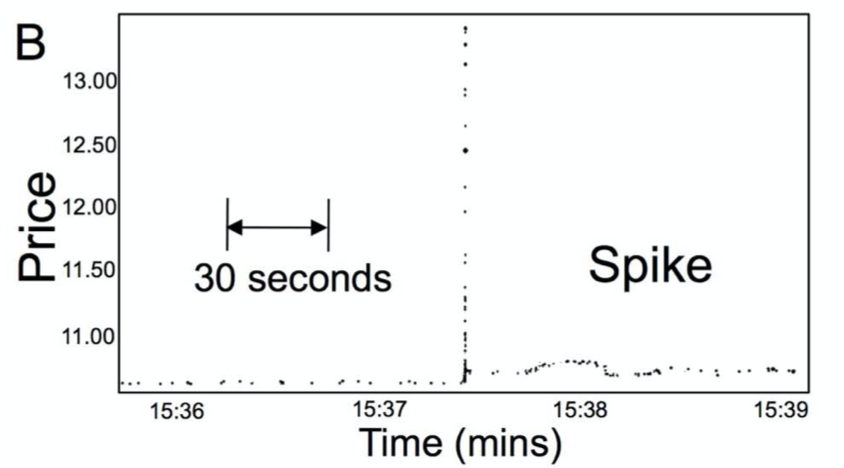
\includegraphics[ height=8cm]{Dissertation/images/Background/johnson price spike.png}
\caption{Price Spike example reproduced from \cite{Johnson}}  
\end{figure} 
\FloatBarrier

The UEE duration is defined as the time period between the first tick and last tick in a certain direction of the price of an UEE event. Johnson et al. shows that these UEE durations generally fall below the human reaction time. In addition, the faster the UEE duration is, the more they become prevalent in the market. This illustrates how the UEE is unlikely to be originate from human traders. 

The reason why the study of these price events is becoming more important is because it can cause large swings in price and affects a firm's assets and value in the market. One example is the crash of an exchange operator called BATS after its IPO on 23rd March 2012. The initial price of the stock is \$15.25 and within 1.5ms the price fell to \$0.0007. BATS then later withdraw their IPO and reported a technical fault due to their high-speed trading algorithm bug. This causes investors and company that has made over \$100 million to return their earnings \cite{BATS}. This is not a single unique event but one of many that has happended in the last decade due to errors in the high-speed trading algorithms. The study of these so-called agents are therefore more important than ever in order to properly regulate the use of these agents and prevent such disaster from happening in the future. 





\chapter{Implementation Overview} 
% \begin{document}

% \section{Introducing realism into BSE}
As introduced by the background, the project intends to investigate the idea of improving an aspect of the simulation to mimic real financial stock exchange environment. To do this, it has taken a step in introducing other players in the financial market and rearrangement of the time step. In the past, the experiments to look at market economics, allocative efficiency and trader agent dominance were done between agents themselves but rarely with other types of players in the market. By conducting the experiments with McG agents, which claims to mimic real financial trading behaviour, may give a better insight on how well the existing trading agents will perform in a realistic market. 

\section{McG's Agents}
A short description of McG can be described in the table below.

\begin{table}[!htbp]
\begin{tabular}{ |m||p{4cm}|p{4cm}| } 
\hline
\textbf{McG Agent}& \textbf{Description}  & \textbf{Parameters}  \\
\hline
\multirow Market maker & Market makers are traders who attempt to earn a profit by taking advantage of the spread in the market & { $v^{-}$ : initial volume }  \\ 
\hline
Liquidity consumer & Liquidity consumer represents large financial institution that makes trading decisions based on re-balancing the portfolio. They only buy or sell in a trading period but not both. & { $h_t$ : remaining volume at time t 
\newline $\phi_t$ : volume at the opposite best price at time t} \\ 
\hline
Momentum trader & Submit order depending on the current momentum ROC. If the ROC is more than a threshold, signifying an upward trend, the agent submits a bid order and an ask order if the trend is going downwards. 
& { $roc_t$ : ROC value at time t
\newline $\kappa$ : threshold of bid and sell
\newline $W_{a,t}$ : Wealth of agent at time t} \\ 
\hline
Mean reversion trader & Mean reversion trader executes order based on the assumption that price level will revert back to their original average. This is by calculating the exponential moving average and updating it at each time step.  
& {$ema_t$ : exponential moving average at time t
\newline $\sigma$ : coefficient 
\newline $v_{m}r$ : initial volume 
\newline $\alpha$ : discount coefficient } \\
\hline
Noise trader & The noise trader are defined so that it captures other activities in the financial market. It randomly execute a sell or a buy with equal probability. & { $\lambda_{m}$ , $\lambda_{l}$, $\lambda_{c}$ : random variables that dictate if the noise trader place a market order, a limit order or cancel an order respectively 
\newline
\newline $v_t$ : volume submit if it places a limit order 
\newline
\newline $\lambda$ : a uniformly generated random value s.t. $\lambda_{crs} + \lambda_{inspr} + \lambda_{spr} + \lambda_{offspr} = 1$}  \\
\hline
\end{tabular}
\end{table}
\FloatBarrier 

\subsection{Market maker}
Market makers are traders who attempt to earn a profit by taking advantage of the spread in the market. The agent executes orders on both bid and ask side of the LOB in each round. * I'm going to ask you on the logic of how Market maker actually makes money. I think I get the idea but I'm not entirely sure yet so I'm skipping this detail bit for now * 

\begin{algorithm}[H]
\DontPrintSemicolon 
\If{$random() > \delta_{mm}$} {
    Cancel any existing order\;
    \If{predict next order is buy} {
    \tcc{$U(a,b)$  function represents value drawn uniformly between $a$ and $b$ }
    Submit sell at best price with volume $V=U(v_{min},v_{max})$\;
    Submit buy at best price with volume $V=U(v^{-})$\;
    }
    \Else{
    Submit buy at best price with volume $V=U(v_{min},v_{max})$\;
    Submit sell at best price with volume $V=U(v^{-})$\;
    }
    \EndIf
  }
\EndIf
Update buy/sell prediction with w-period rolling mean\; 
\caption{{\sc Market maker adapted from McG (4.1) \cite{McGroarty}} }
\label{algo:max}
\end{algorithm}

\subsection{Liquidity consumer}
Liquidity consumer represents large financial institution that makes trading decisions based on re-balancing the portfolio. The agent decides to buy or sell at the start of the day with a specific volume to minimize price impact and trading costs. At the start of the day, the agent decides, with equal probability, to sell or buy for the whole day.

\begin{algorithm}[H]
\DontPrintSemicolon 
\If{start of the day} {
    \If{$random() > 0.5$} {
    Decides to Buy\;
    }
    \Else{
    Decides to Sell;\
    }
    \EndIf
    Execute initial market order with volume $h_0 = U(h_{min},h_{max})$\;  
  }
\EndIf

\If{$random() < \delta_{lc}$} {
    \tcc{$\phi_t = $  the volume at the opposite best price at time t}
    \tcc{$h_t = $ is the remaining volume at time t}
    \If{$h_t \leq \phi_t$} {
    Submit market order with volume $v_t = h_t$\;
    }
    \Else{
    Submit market order with volume $v_t = \phi_t$;\
    }
    \EndIf
    $h_t = h_t - 1$\;  
  }
\EndIf
\caption{{\sc Liquidity consumer adapted from McG (4.2) \cite{McGroarty} }}
\label{algo:max}
\end{algorithm}

\subsection{Momentum trader}
A momentum trader trades depending on the rate of change in the price movement. The trader will take a long position if the price has recently been rising and a short position otherwise. The calculation of Rate of Change (ROC) is given by: 

    \[ roc_t = \frac{p_t - p_{t-n_r}}{p_{t-n_r}} \]
    
When $roc_t$ is greater than some threshold $\kappa$, the agent submits a bid order with the volume described as:

    \[ v_t = \abs{roc_t} * W_{a,t} \]
    
where $W_{a,t}$ is the wealth of the agent at time $t$. 

\begin{algorithm}[H]
\DontPrintSemicolon 
\If{$random() < \delta_{mt}$} {
    \If{$roc_t \ge \kappa$} {
    Submit market buy order with volume $v_t = \abs{roc_t} * W_{a,t}$\;
    }
    \uElseIf{$roc_t \leq -\kappa$}{
    Submit market sell order with volume $v_t = \abs{roc_t} * W_{a,t}$;\
    }
    \EndIf
  }
\EndIf
Update ROC $roc_t = \frac{p_t - p_{t-n_r}}{p_{t-n_r}}$\;  
\caption{{\sc Momentum trader adapted from McG (4.3) \cite{McGroarty} } }
\label{algo:max}
\end{algorithm}


\subsection{Mean reversion trader}
Mean reversion trader executes order based on the assumption that price level will revert back to their original average. This means that they play a long position when the current price is below the average and short when it is above. The exponential moving average is given by: 

\[ ema_t = ema_{(t-1)} - \alpha(p_t - ema_{(t-1)}) \] where $p_t$ is price at time $t$ and $\alpha$ is a discount coefficient that adjust the recency bias. If the current price $p_t$ is $k$ standard deviation above $ema_t$, the agent submits a sell order and a buy order if it is $k$ standard deviation below $ema_t$. The volume is denote by $v_mr$.

\begin{algorithm}[H]
\DontPrintSemicolon 
\If{$random() < \delta_{mr}$} {
    \If{$p_t - ema_t \ge k\sigma_t$} {
    Submit sell just inside best ask with $v_t = v_mr$\;
    }
    \uElseIf{$ema_t - p_t \leq k\sigma_t$}{
    Submit buy just inside best ask with $v_t = v_mr$\;
    }
    \EndIf
  }
\EndIf
Update $ema_t$ = $ema_{(t-1)} - \alpha(p_t - ema_{(t-1)}$
\caption{{\sc Mean reversion trader adapted from McG (4.4) \cite{McGroarty}} }
\label{algo:max}
\end{algorithm}


\subsection{Noise Trader} 
The noise trader are defined so that it captures other activities in the financial market. It randomly execute a sell or a buy with equal probability. Once they decide, they either place a market order or limit order or cancel existing order with probability $\lambda_{m}$, $\lambda_{l}$ and $\lambda_{c}$ respectively. If it does submit an order, the volume is drawn from a log-normal distribution described by:
\[ v_t = exp(\mu + \sigma u_v) \]
where $\mu$ and $\sigma$ is mean and standard deviation of the $v_t$s natural logarithm. $u_v$ is a value uniformly drawn between 0 and 1. 

In the case where a limit order is chosen, the price is determined by these four extended possibilities given by: 
\begin{itemize}
  \item With probability $\lambda_{crs}$ agent places an order with the opposite best price in order to make the exchange execute immediately. If not, the order sits on the LOB. 
  \item With probability $\lambda_{inspr}$ the agent places an order with price $p_{inspr}$ uniformly drawn between best bid and best ask (the spread). 
  \item With probability $\lambda_{spr}$ the agent places an order with best price on their side of the book (determined eariler if bid or ask)
  \item With probability $\lambda_{offspr}$ places an order with price distributed with:  
  \[ xmin_{offspr} * (1-u_0)^{-\frac{1}{\beta - 1}} \]
\end{itemize}
The condition is that $\lambda_{crs} + \lambda_{inspr} + \lambda_{spr} + \lambda_{offspr} = 1$ to prevent spurious price movement in addition to the volume $v_mr$ limited up to half of the available volume at the side of the book. 

\begin{algorithm}[H]
\DontPrintSemicolon 
\If{$random() < \delta_{nt}$} {

    \If{$random() < 0.5$} {
    Decides to Sell\;
    }
    \Else{
    Decides to Buy;\
    }
    \EndIf
    Generate $U(0,1)$ to determine action,$\lambda_{m}$ , $\lambda_{l}$ and $\lambda_{c}$.
    
    \Switch{action}
    {
        \Case{Submit Market Order}{Submit market order with volume calculated by $v_nt = exp(\mu + \sigma u_v)$}
        \Case{Submit Limit Order}{
        Generate $U(0,1)$ to determine action,$\lambda_{crs}$ , $\lambda_{inspr}$,$\lambda_{spr}$  and $\lambda_{cspr}$.
            \Switch{action}
            {
                \Case{Crossing Limit Order }{Submit limit order at opposing best price with volume $v_nt$ }
                \Case{Inside spread limit order }{Generate random value with $U(BestBid,BestAsk)$ with volume $v_nt$}
                \Case{Spread Limit Order }{Submit limit order at the best price with volume $v_nt$}
                \Case{Off-spread Limit Order }{Generate a random price value using $xmin_{offspr} * (1-u_0)^{-\frac{1}{\beta - 1}}$ }
            
            }
        }
        \Case{Cancel Existing Order}{Cancel the oldest order previously submitted.}
    }
  }
\EndIf
\caption{{\sc Noise trader adapted from McG (4.5) \cite{McGroarty}} }
\end{algorithm}

\section{BSE and McG price assignments}
In the BSE, traders are clearly labeled as either a Buyer or a Seller where they will be submitting only a bid and an ask order in each round. In addition, in the beginning of the trading period, the agents will receive a customer order or "assignments" notifying them to trade at a specific price and quantity. Then agents then can use this information as a factor to make decisions on their orders. Another purpose of the assignment is that they set the equilibrium price of the market and demand-supply curve. 

McG's model does not rely on the assignments like the BSE. It relies on the ``best price" of each side of the book being available in any given time. This is an assumption that matches the real world market since the current spread will always be immediately available if the market is open. 

\begin{figure}[h]
\caption{BSE market diagram} 
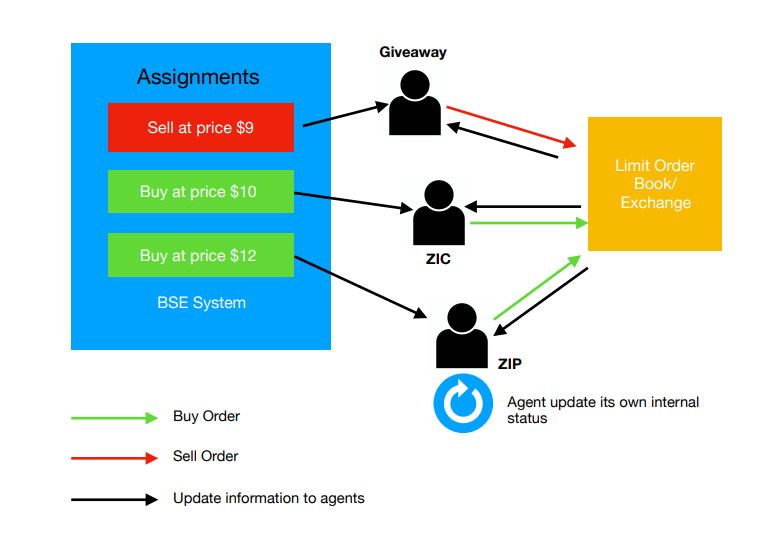
\includegraphics[ height=8cm]{BSE_figure}
\caption{McG's market model diagram} 
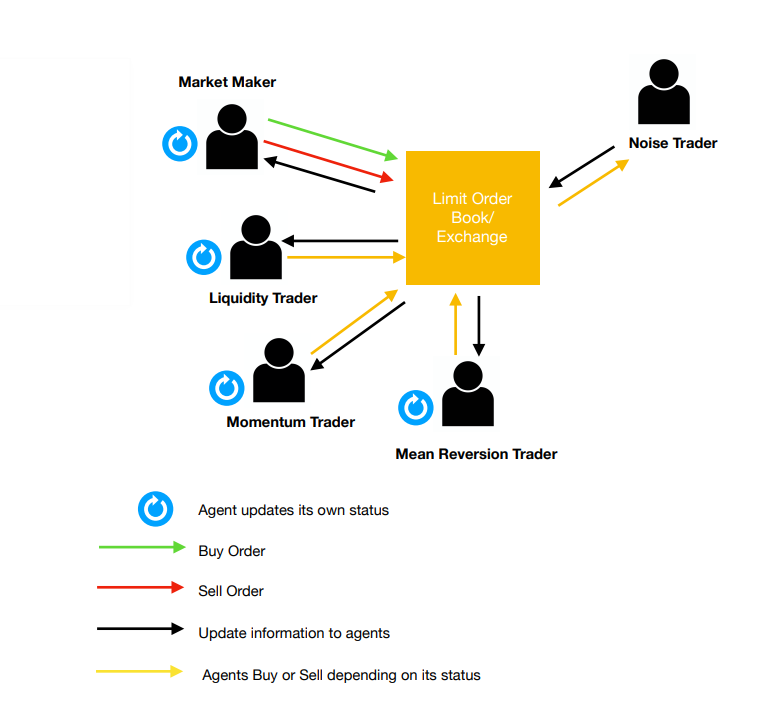
\includegraphics[width=\textwidth, height=10cm]{McGroarty_figure}
\end{figure} 

In the new implementation which this project is trying to achieve is finding a way to integrate these two systems so that the McG agents will be able to mimic the real market environment for the agents such as ZIP, ZIC and AA implemented in the BSE. This implementation requires a few changes.

\begin{itemize}
    \item  \textbf{Quantity} : The current version of the BSE does not support orders with quantity more than 1.This has to be change because all of McGroarty et al. agents require their market to be able to receive orders with quantity more than 1. 
    \item  \textbf{Accepting more than one order per round}: In the current version, the BSE only accepts one order randomly from an agent in a time step. Agents such as the Market maker must be able to submit more than one order in every round. 
    \item \textbf{Deleting an order} : The current version of the BSE does not fully support an agent cancelling their order directly. This has to be implemented as a part of the system since McGroarty et al. agents are capable of cancelling an order.
\end{itemize} 

\section{The availability of Best Price in the BSE}
Some of McG's agents depend on the "best price" of a side of the book in order to submit an order. However, unlike the real exchange market, the BSE does not always provide that, more specifically in the beginning of the trading day. This means that there must be some unavoidable modifications to the McG's agents condition regarding order submission. There are multiple approaches in which the project will explore, including:

\begin{itemize}
    \item \textbf{Not submitting if only the worst price is available} This simple makes sense because if the agent submits at the worst price, it is essentially making a loss, thus not a smart decision in any case. By skipping the round and waiting for the right market price is what any normal trader would do. 
    
    \item \textbf{Using the worst price with linear modification} * I'm not sure how to do this one yet so I'll be writing this one later 
\end{itemize} 


% \end{document} 

\chapter{Base Line results and Initial tests} 
Before the agents described in the Chapter 2 will be implemented, we will first implement a new BSE system that can handle more complex order types and adapt the time system. This chapter will consists of Base Line results, both taken from previous literature and from running in the original BSE. These Base Line results will then be used to compare the results from running each agent (ZIP, ZIC and Sniper) in the new system. If the behaviour is similar, then we can conclude that the system has been implemented correctly. However, as the system is developed, some parameters of the agents may have to be adapted, but the overall behaviour will be the same. 

\section{Base Line Results} 
Base Line results act as a standard which can be expected from the agents by running in a homogeneous market. These results are the indicator, apart from the unit and integration testing, that ensures the market is stabilized and performs as expected. The following graphs will illustrate the transaction prices in each homogeneous market. The following results are from running in the original BSE with equilibrium price of 100 in a homogeneous market with 31 agents on each side of the book. The period length 180 is chosen to match those in previous literature in order to compare the results of the current implementation and previous established results. 

In addition, the experiments will compare \textbf{Smith's alpha} which is the standard deviation of the transaction price around the equilibrium. The equation is given by 

\begin{equation}
\alpha = \frac{100}{P_0}\sqrt{\sum_{t=0}^{n} \frac{(P_t - P_0)^2}{|T|} }
\end{equation}
where $P_0$ = equilibrium price 
\newline $P_t$ = price at transaction t 
\newline $T$ = number of total transactions in the run
\newline $n$ = $n_{th}$ transaction in the run

\begin{table}[h]
\centering
\begin{tabular}{ |m||p{4cm}|} 
\hline
\textbf{Base Line agents experiment}& \textbf{Smith's alpha value} \\
\hline
\hline
Kaplan's Sniper & 49.73 \\ 
\hline
ZI-C & 63.5\\ 
\hline
ZI-P & 24.8 \\ 
\hline
\end{tabular}
\caption{Smith's alpha value of each base line experiment}  
\end{table}
\FloatBarrier

The ZI-P agent has the lowest Smith's alpha value out of the three agents because it is the best at convergence to the equilibrium while the ZI-C agent has the highest value because the oscillation in its transaction prices is very high. 

\subsection{Kaplan's Sniper}
The Kaplan's Sniper is one of the agents implemented in the original version of the BSE. The sniper waits until near the end of the period, then submits or ``snipe" its order. This is consistent with Figure \ref{fig:Sniper_org_all} where the transaction only occurs near the end of the time period or when $t = 160$.

\begin{figure}[h]
  \begin{subfigure}[b]{0.5\textwidth}
    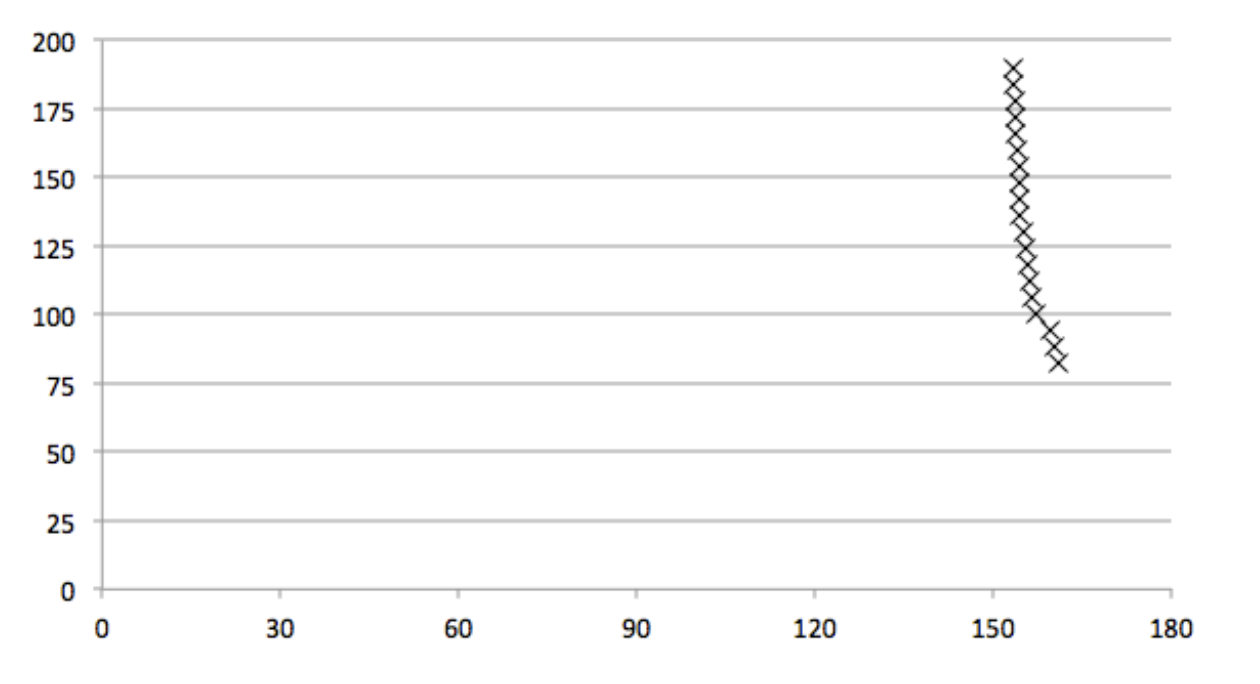
\includegraphics[width=7cm, height=7cm]{Dissertation/images/base_line/SNPR_lit.png}
    \caption{Previous Literature result \cite{BSE_lit}} 
    \label{fig:Sniper_lit}
  \end{subfigure}
  %
  \begin{subfigure}[b]{0.5\textwidth}
    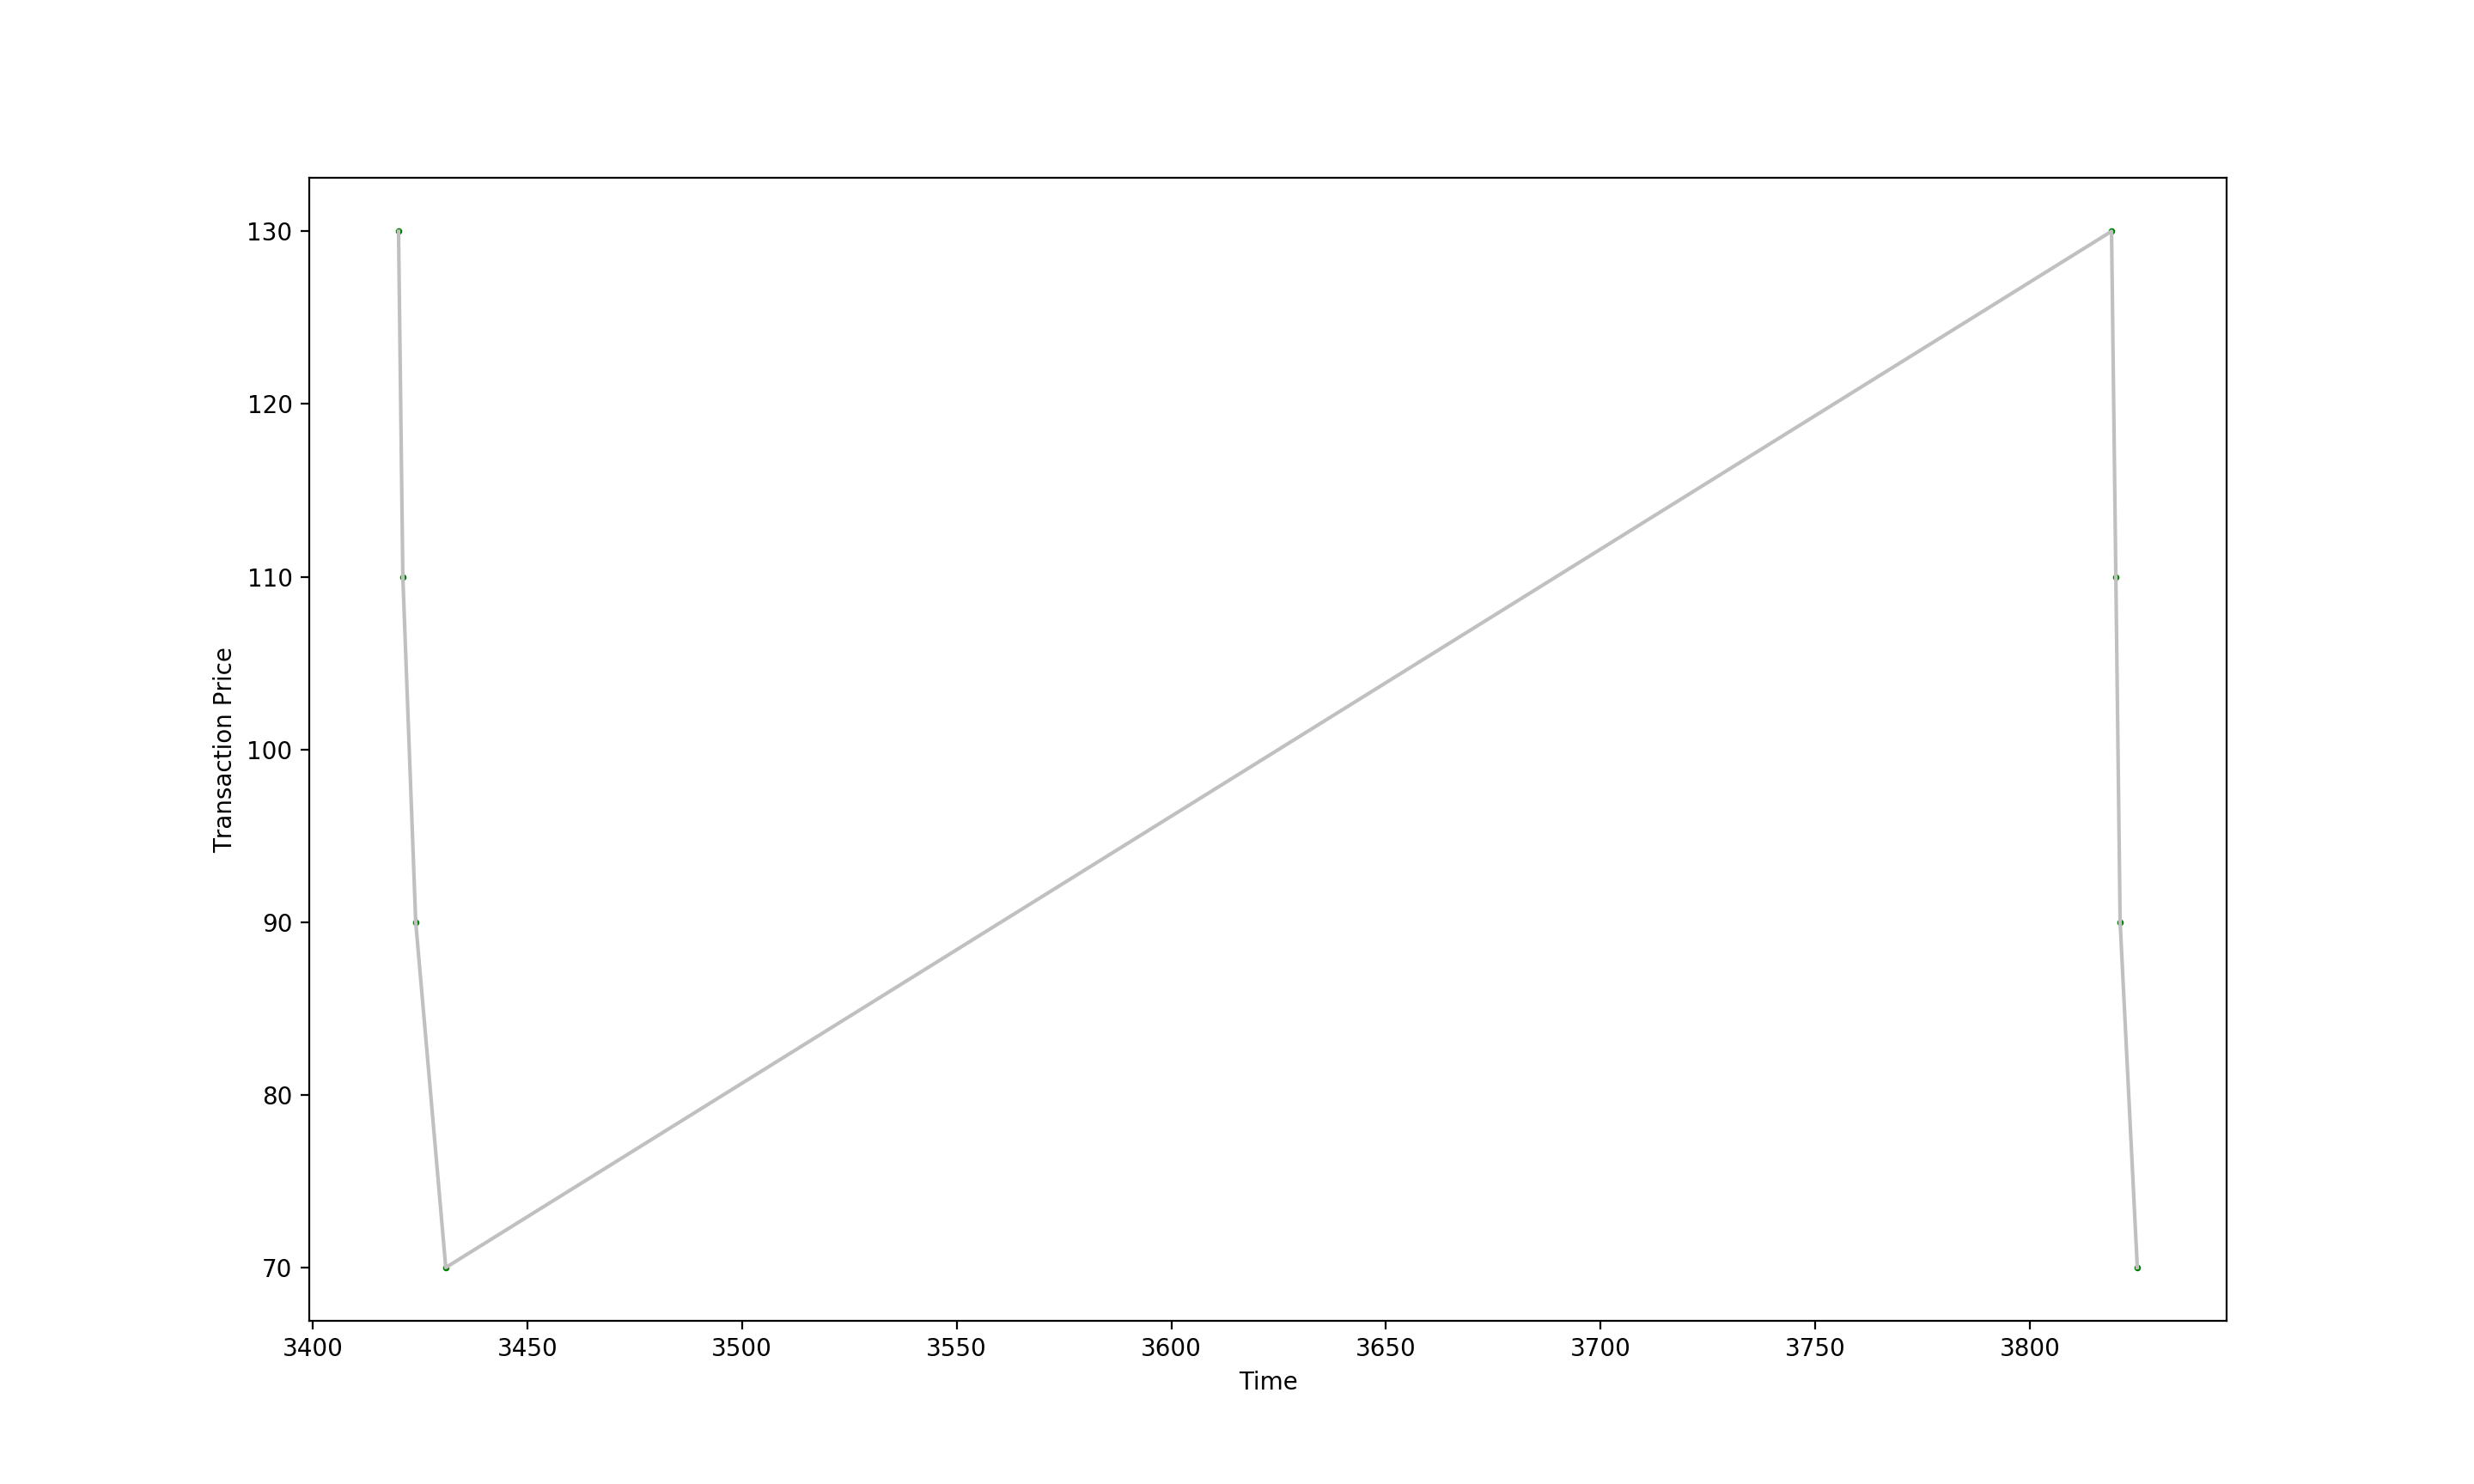
\includegraphics[width=7cm, height=7cm]{Dissertation/images/base_line/sniper.png}
    \caption{Original BSE result}
    \label{fig:Sniper_original}
  \end{subfigure}
\caption{Comparison of 62 Sniper homogeneous transaction diagram with 100 price equilibrium from previous literature and original BSE result} 
\label{fig:Sniper_org_all}
\end{figure}
\FloatBarrier

\subsection{ZI-C}
ZI-C or Zero-Intelligence Constrained is another agent implemented in the original BSE. An expected behaviour of a market consisting of only ZI-C agents is a non-convergence transaction price. This is consistent with the Figure \ref{fig:ZIC_org_all} below where at the end of the transaction period, the price does not converge to the equilibrium but instead exhibits a volatile price changes over the time period. 

\begin{figure}[h]
  \begin{subfigure}[b]{0.5\textwidth}
    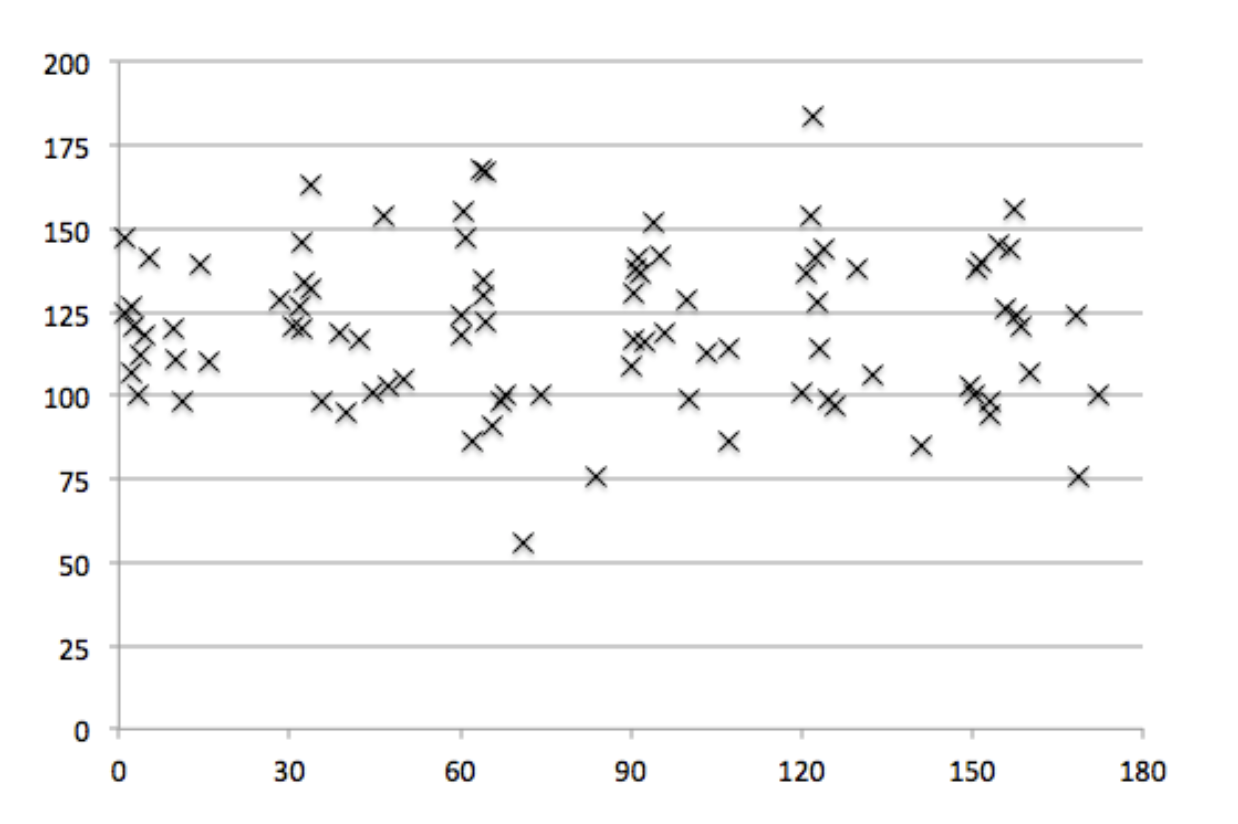
\includegraphics[width=7cm, height=7cm]{Dissertation/images/base_line/zic_lit.png}
    \caption{Previous Literature result \cite{BSE_lit}} 
    \label{fig:1}
  \end{subfigure}
  %
  \begin{subfigure}[b]{0.5\textwidth}
    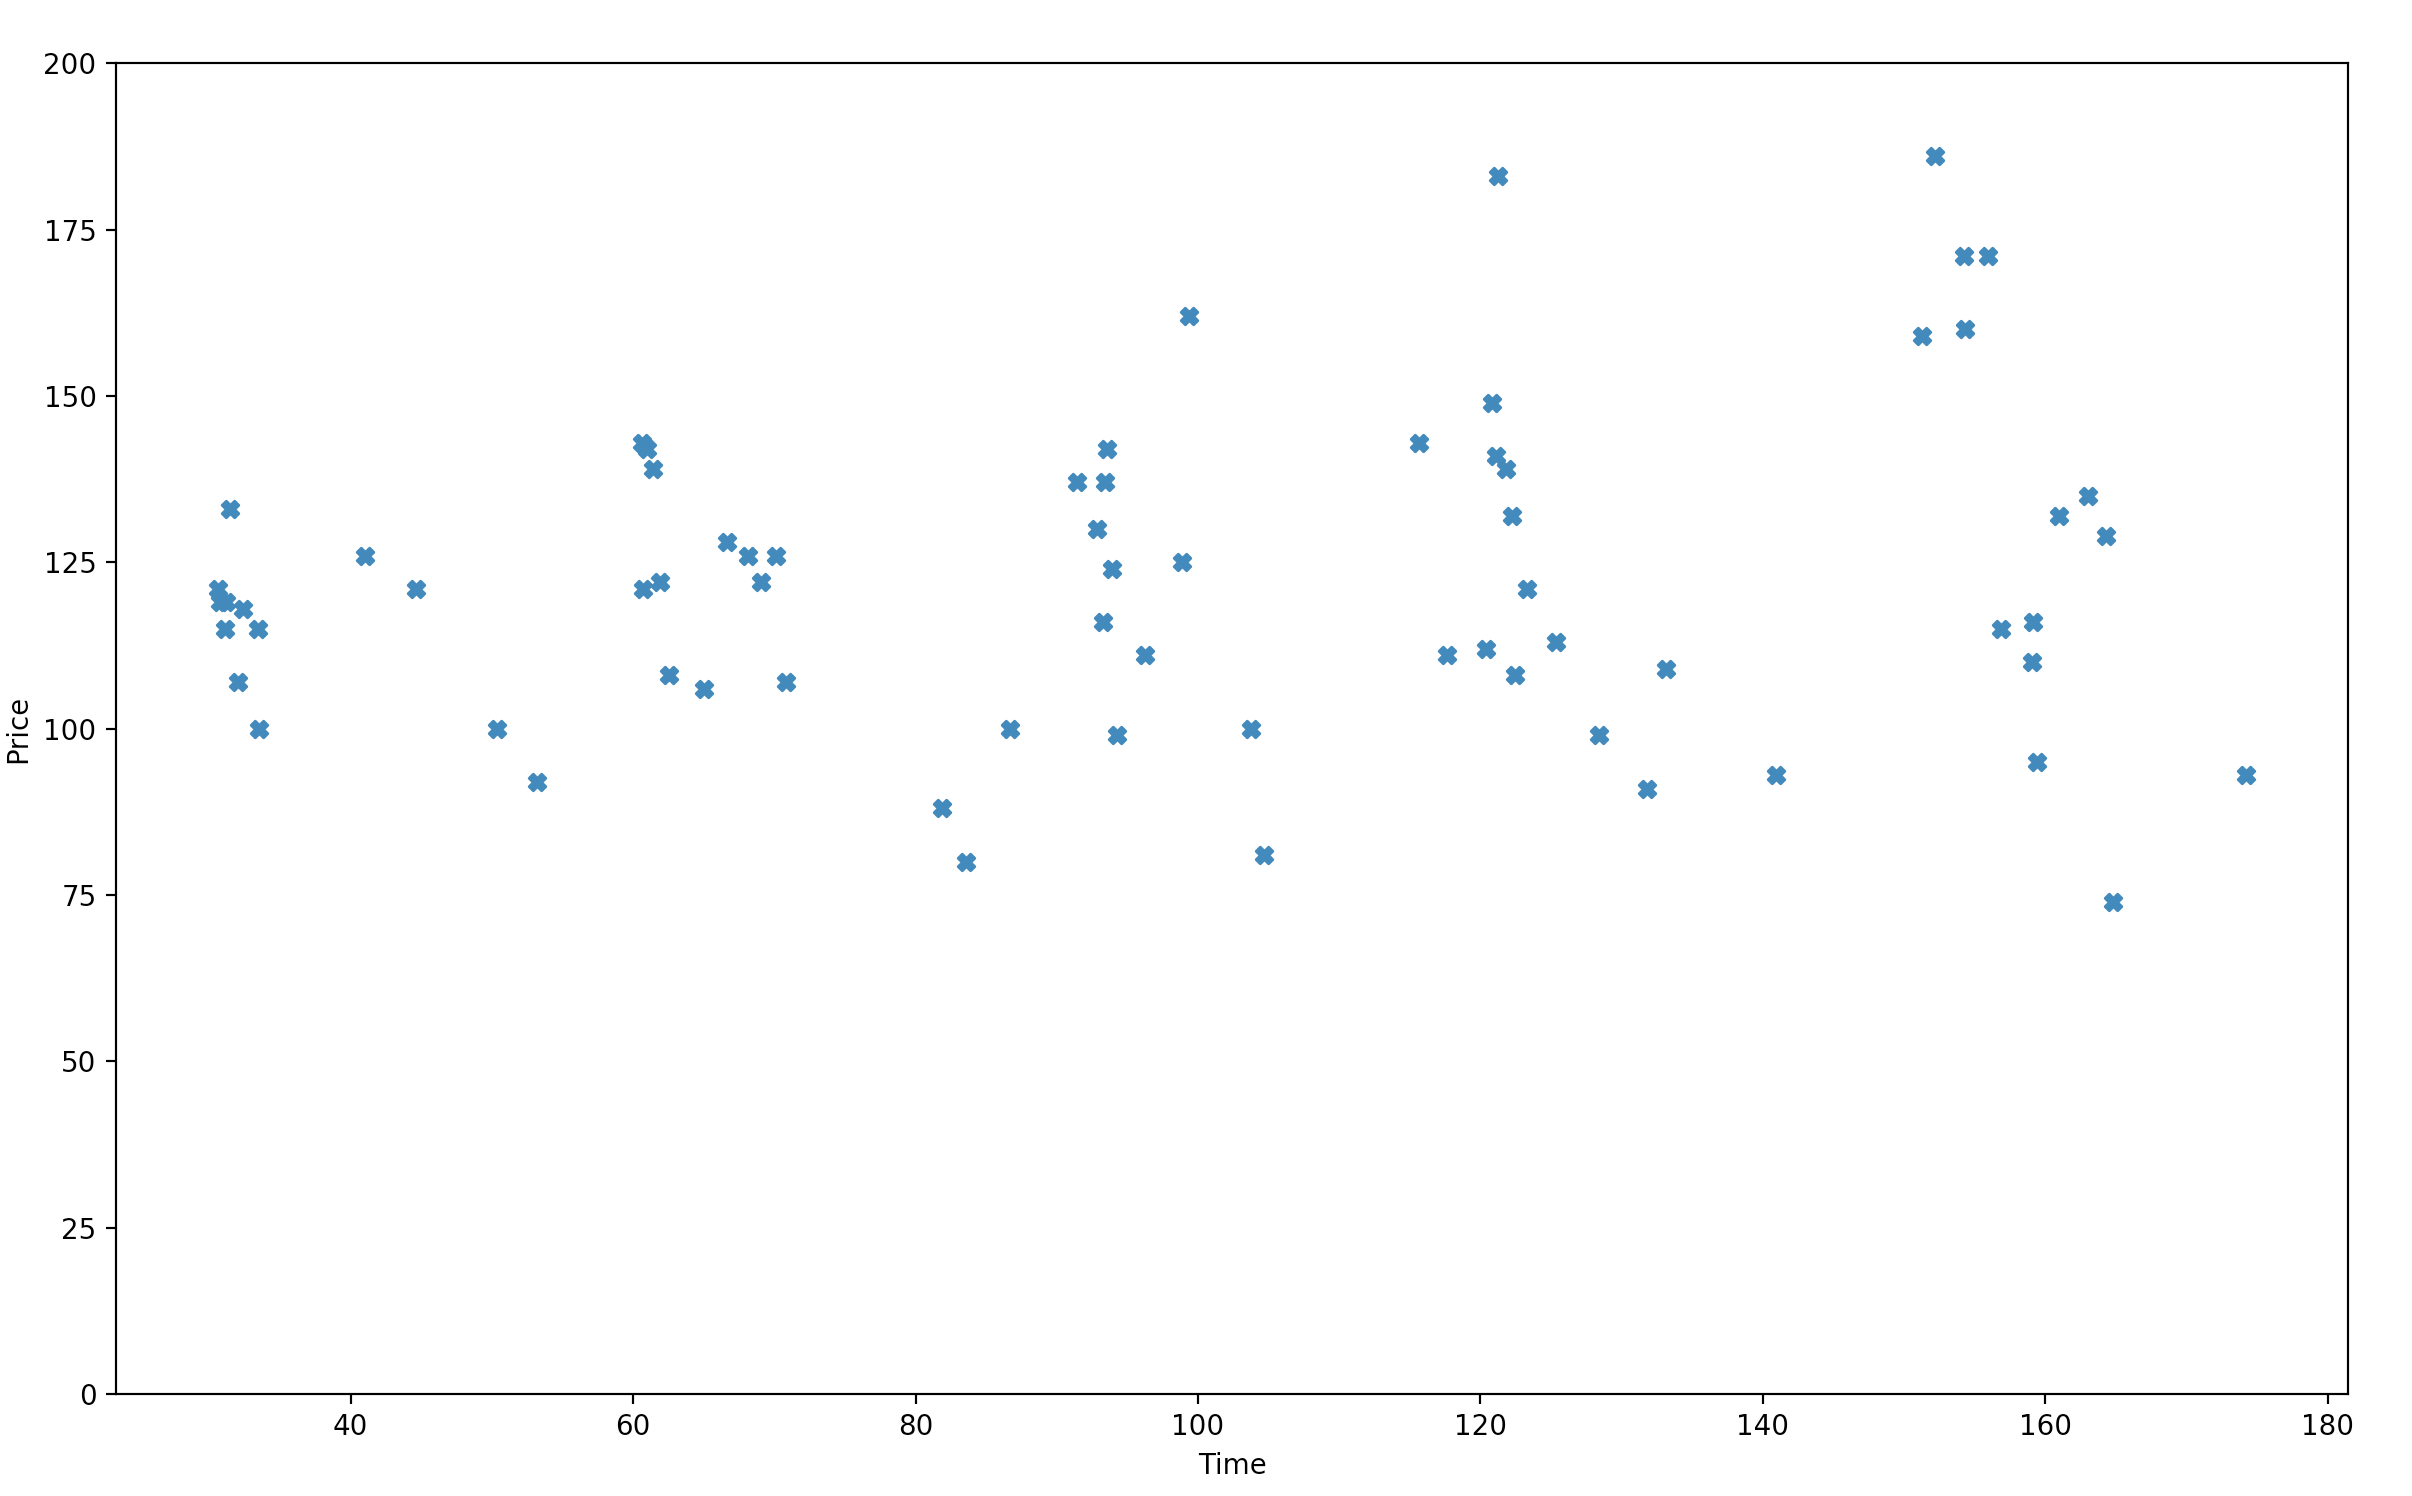
\includegraphics[width=7cm, height=7cm]{Dissertation/images/base_line/ZIC.png}
    \caption{Original BSE result}
    \label{fig:2}
  \end{subfigure}
\caption{Comparison of 62 ZI-C homogeneous transaction diagram with 100 price equilibrium from previous literature and original BSE result} 
\label{fig:ZIC_org_all}
\end{figure}
\FloatBarrier


\subsection{ZI-P}
ZI-P or Zero-Intelligence Plus is the agent that, in a homogeneous market, does produce a market where the transaction price which converges to the equilibrium. A market of ZI-P agents is a good indicator to test the market structure and functions. In the Figure \ref{fig:ZIP_org_all} below, the transaction price first fluctuates early in the transaction period but then converges towards 100 in the end of the session.  

\begin{figure}[h]
  \begin{subfigure}[b]{0.5\textwidth}
    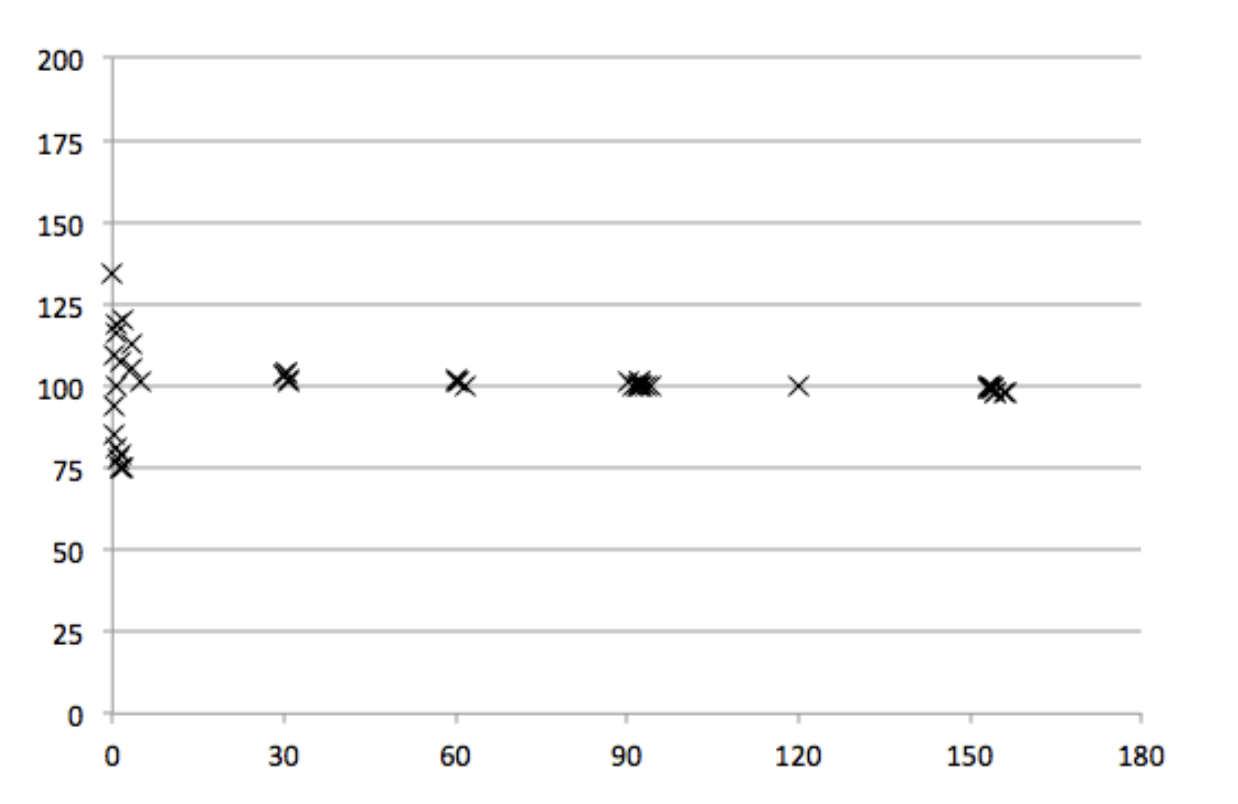
\includegraphics[width=7cm, height=7cm]{Dissertation/images/base_line/zip_lit.png}
    \caption{Previous Literature result \cite{BSE_lit}} 
    \label{fig:1}
  \end{subfigure}
  %
  \begin{subfigure}[b]{0.5\textwidth}
    \includegraphics[width=7cm, height=7cm]{Dissertation/images/base_line/zip.png}
    \caption{Original BSE result}
    \label{fig:2}
  \end{subfigure}
\caption{Comparison of 62 ZI-P homogeneous transaction diagram with 100 price equilibrium from previous literature and original BSE result} 
\label{fig:ZIP_org_all}
\end{figure}
\FloatBarrier


\section{Results after implementing complex order types} 
These results are from tests ran with the same configuration as the Base Line tests in section 3.1. These tests are ran after the LOB has been re-configured to be able to accept more than one type of order (Market Order as well as Limit Order) in addition to more than one quantity. The tests are ran with the same time step as the original BSE. Table 3.2 illustrates the similarities between the alpha values between each 2 configurations which is the evidence that the agents are acting as expected.  

\begin{table}[h]
\centering
\begin{tabular}{ |m||p{4cm}|p{4cm}|} 
\hline
\textbf{Agents}& \textbf{Base Line Smith's alpha value}& \textbf{Complex order type Smith's alpha value} \\
\hline
\hline
Kaplan's Sniper & 49.73  & 49.51 \\ 
\hline
ZI-C  & 63.5 & 64.3\\ 
\hline
ZI-P & 24.8 & 22.4 \\ 
\hline
\end{tabular}
\caption{Smith's alpha value after implementing complex order types}  
\end{table}
\FloatBarrier


\subsection{Kaplan's Sniper}
As expected, the Sniper only submits orders near the end of the session, which makes the first transactions only appear after $t = 160$.  
\begin{figure}[h]
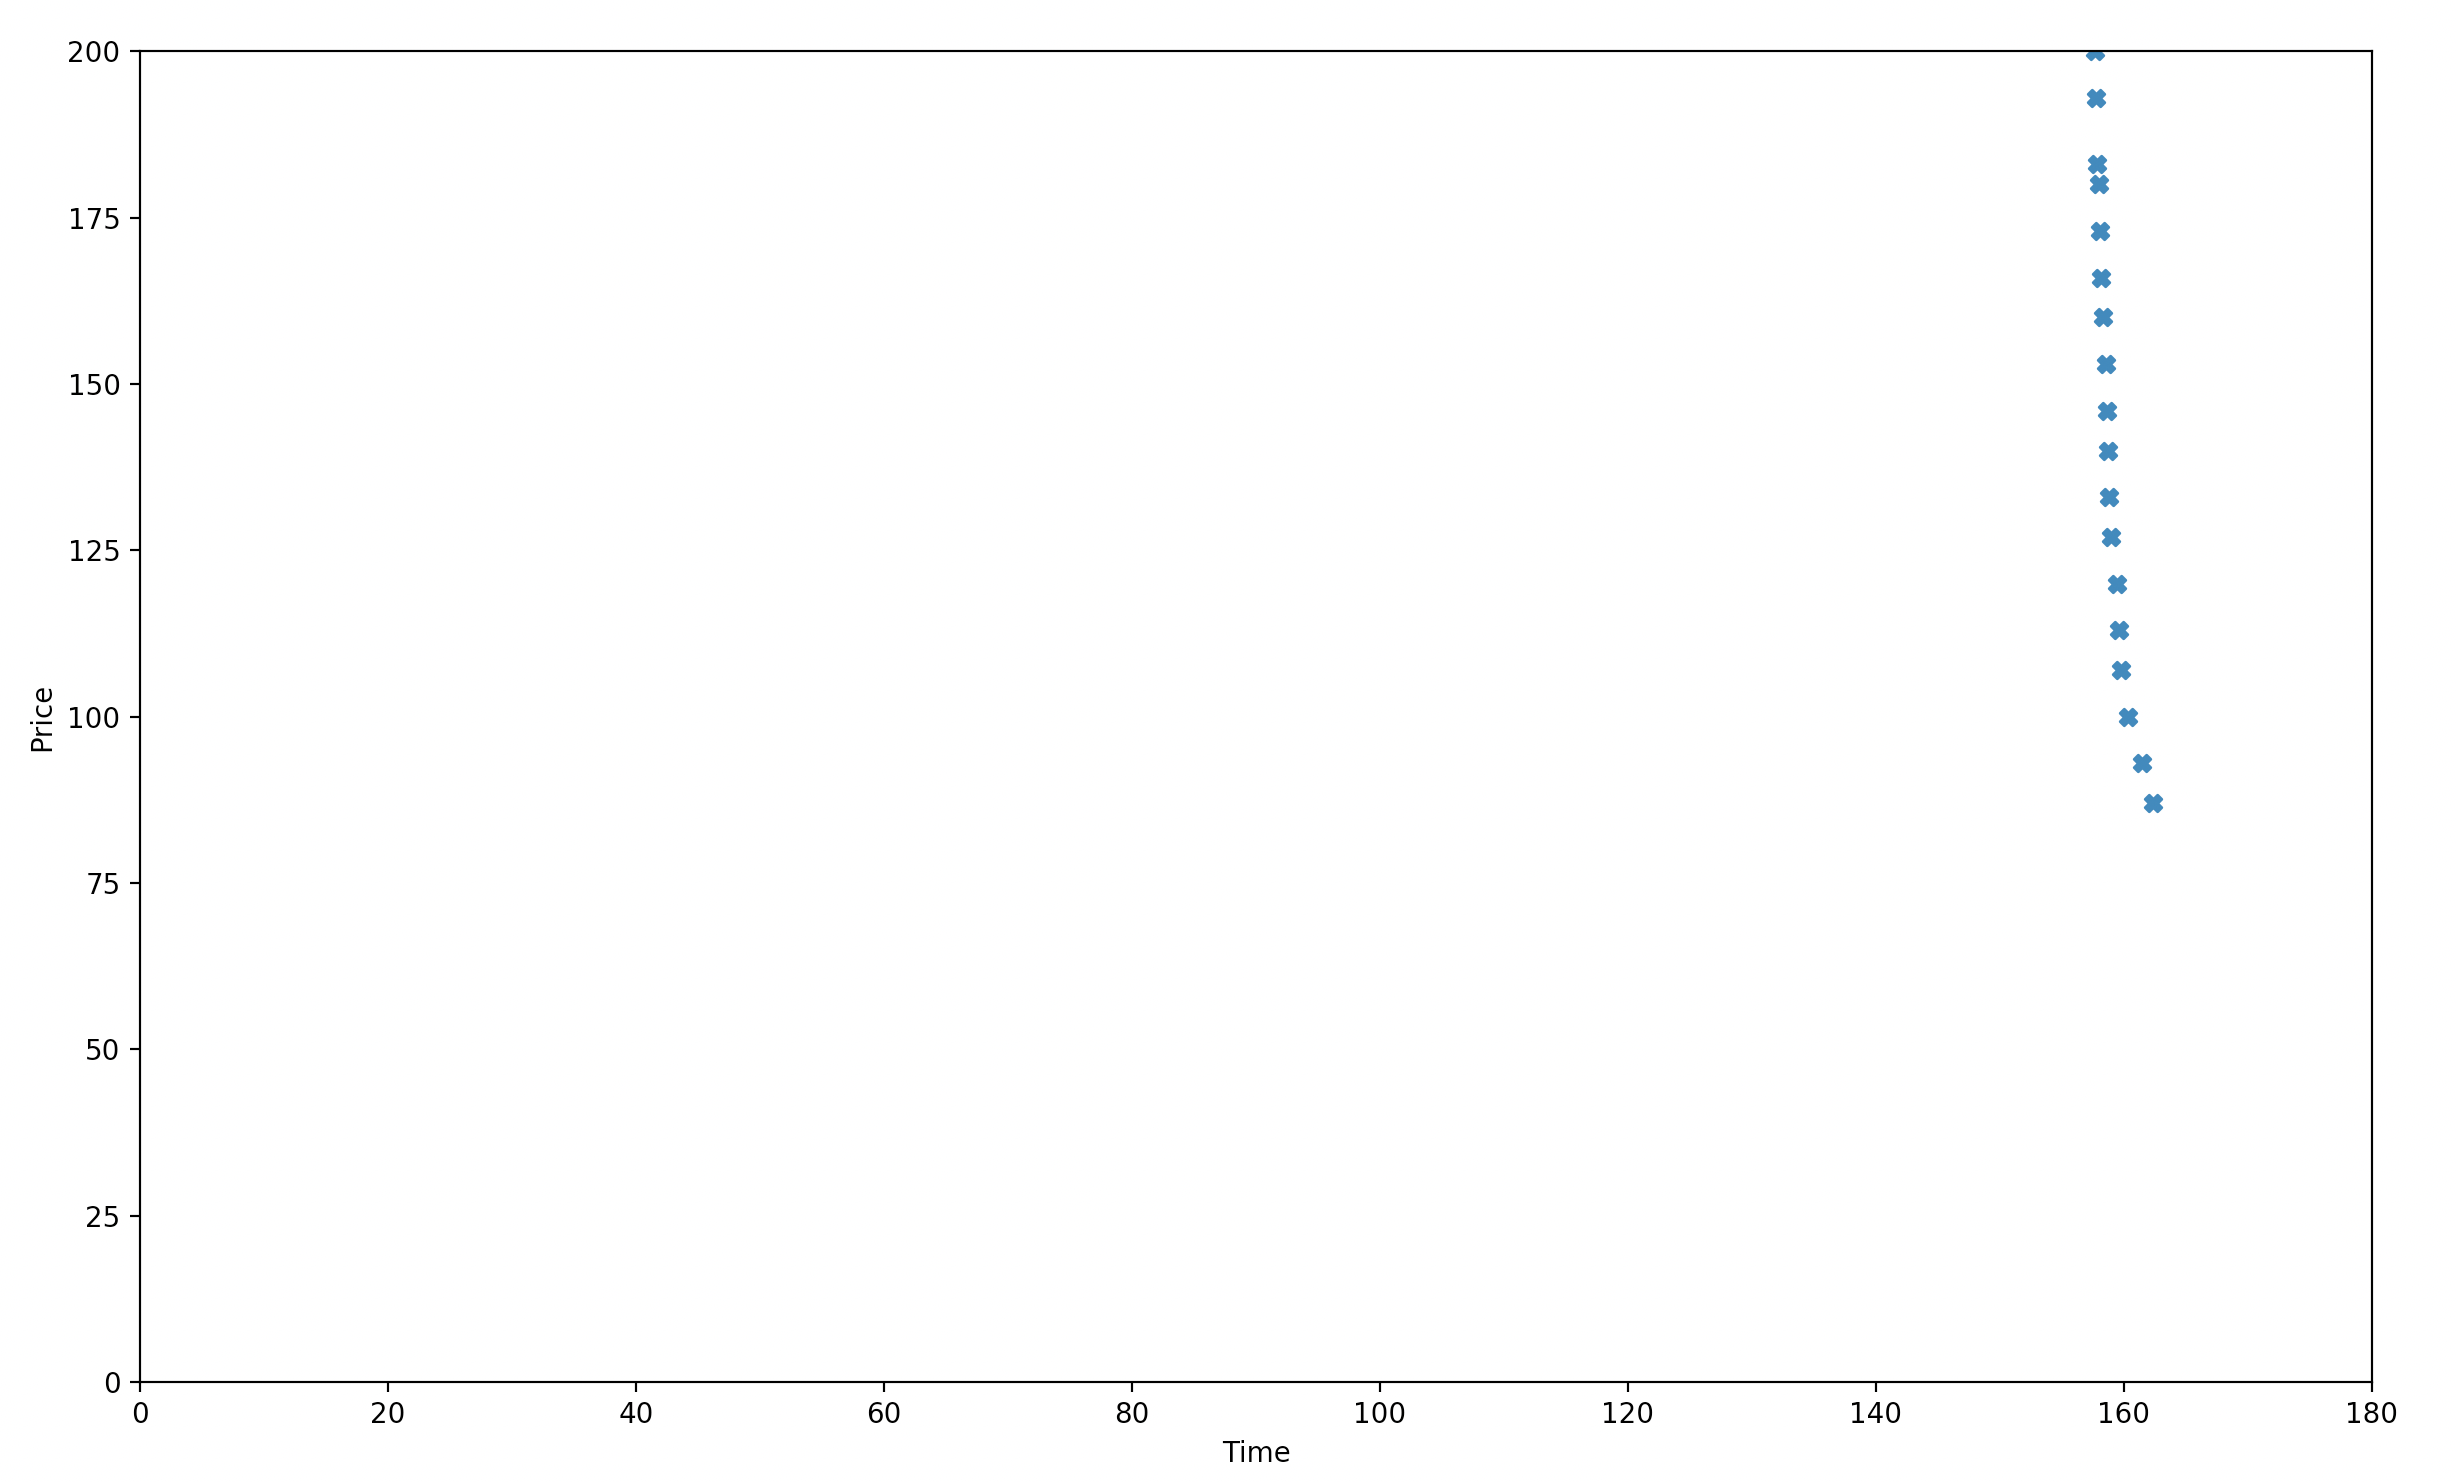
\includegraphics[ height=7cm]{Dissertation/images/change1/snpr.png}
\caption{62 Sniper agents homogeneous market transaction diagram with 100 price equilibrium from complex order types implementation} 
\end{figure} 
\FloatBarrier

\subsection{ZI-C}
ZIC's behaviour in the new LOB is still similar to the one ran in the original BSE. The transaction price does not converge in any period of the session. 

\begin{figure}[h]
\includegraphics[ height=7cm]{Dissertation/images/change1/zic.png}
\caption{62 ZI-C agents homogeneous market transaction diagram with 100 price equilibrium from complex order types implementation} 
\end{figure} 
\FloatBarrier

\subsection{ZI-P}
ZIP illustrates a convergence to the 100 equilibrium as expected. 

\begin{figure}[h]
\includegraphics[ height=7cm]{Dissertation/images/change1/zip.png}
\caption{62 ZI-P agents homogeneous market transaction diagram with 100 price equilibrium from complex order types implementation} 
\end{figure} 
\FloatBarrier

\section{Results after implementing McG action step} 
This section illustrate the results with same test configurations on the BSE with McG action step. The McG action step is similar to the BSE except that it does not divide the individual time-step by the number of buyers and sellers then select them randomly. The McG action-step loops through every trader in each step, allowing the trader to have a chance to act in all the time steps. The time period selected is 180 * 62 = 11,160 which is equivalent to the 180 time step in original BSE time-step. In addition, the interval is changed to be 10\% of the time-step for the customer order (price assignments) which is 1,860 in the McG and 30 in the original BSE. The results of the tests are illustrated below. 

\begin{table}[h]
\centering
\begin{tabular}{ |m||p{4cm}|p{4cm}|p{4cm}|} 
\hline
\textbf{Agents}& \textbf{Base Line Smith's alpha value} & \textbf{Smith's alpha value for section 3.2} & \textbf{Implemented McG action-step Smith's alpha value} \\
\hline
\hline
Kaplan's Sniper & 49.73  & 49.51 & 50.1 \\ 
\hline
ZI-C & 63.5 & 64.3 & 67.3\\ 
\hline
ZI-P & 24.8 & 22.4 & 25.4 \\ 
\hline
\end{tabular}
\caption{Smith's alpha value after implementing McG action step}  
\end{table}
\FloatBarrier

\subsection{Kaplan's Sniper}
As expected, the Sniper only submits orders near the end of the session, which makes the first transactions only appear after $t = 9000$. However, Figure \ref{fig:sniper_wrong} suggests that the behaviour of the Sniper agent is not entirely the same as there are similar transactions from the agents submitting two sets of similar orders in the end of the period. This is partly because the gap between 9,000 - 11,160 is much higher than 160 - 180 in previous experiments. Therefore, the agents have time to submit two different sets of orders. This suggests that there needs to be some adaptation to the agent's values in order to retain the behaviour it has in the Base Line experiment Figure \ref{fig:Sniper_org_all}. 

\begin{figure}[h]
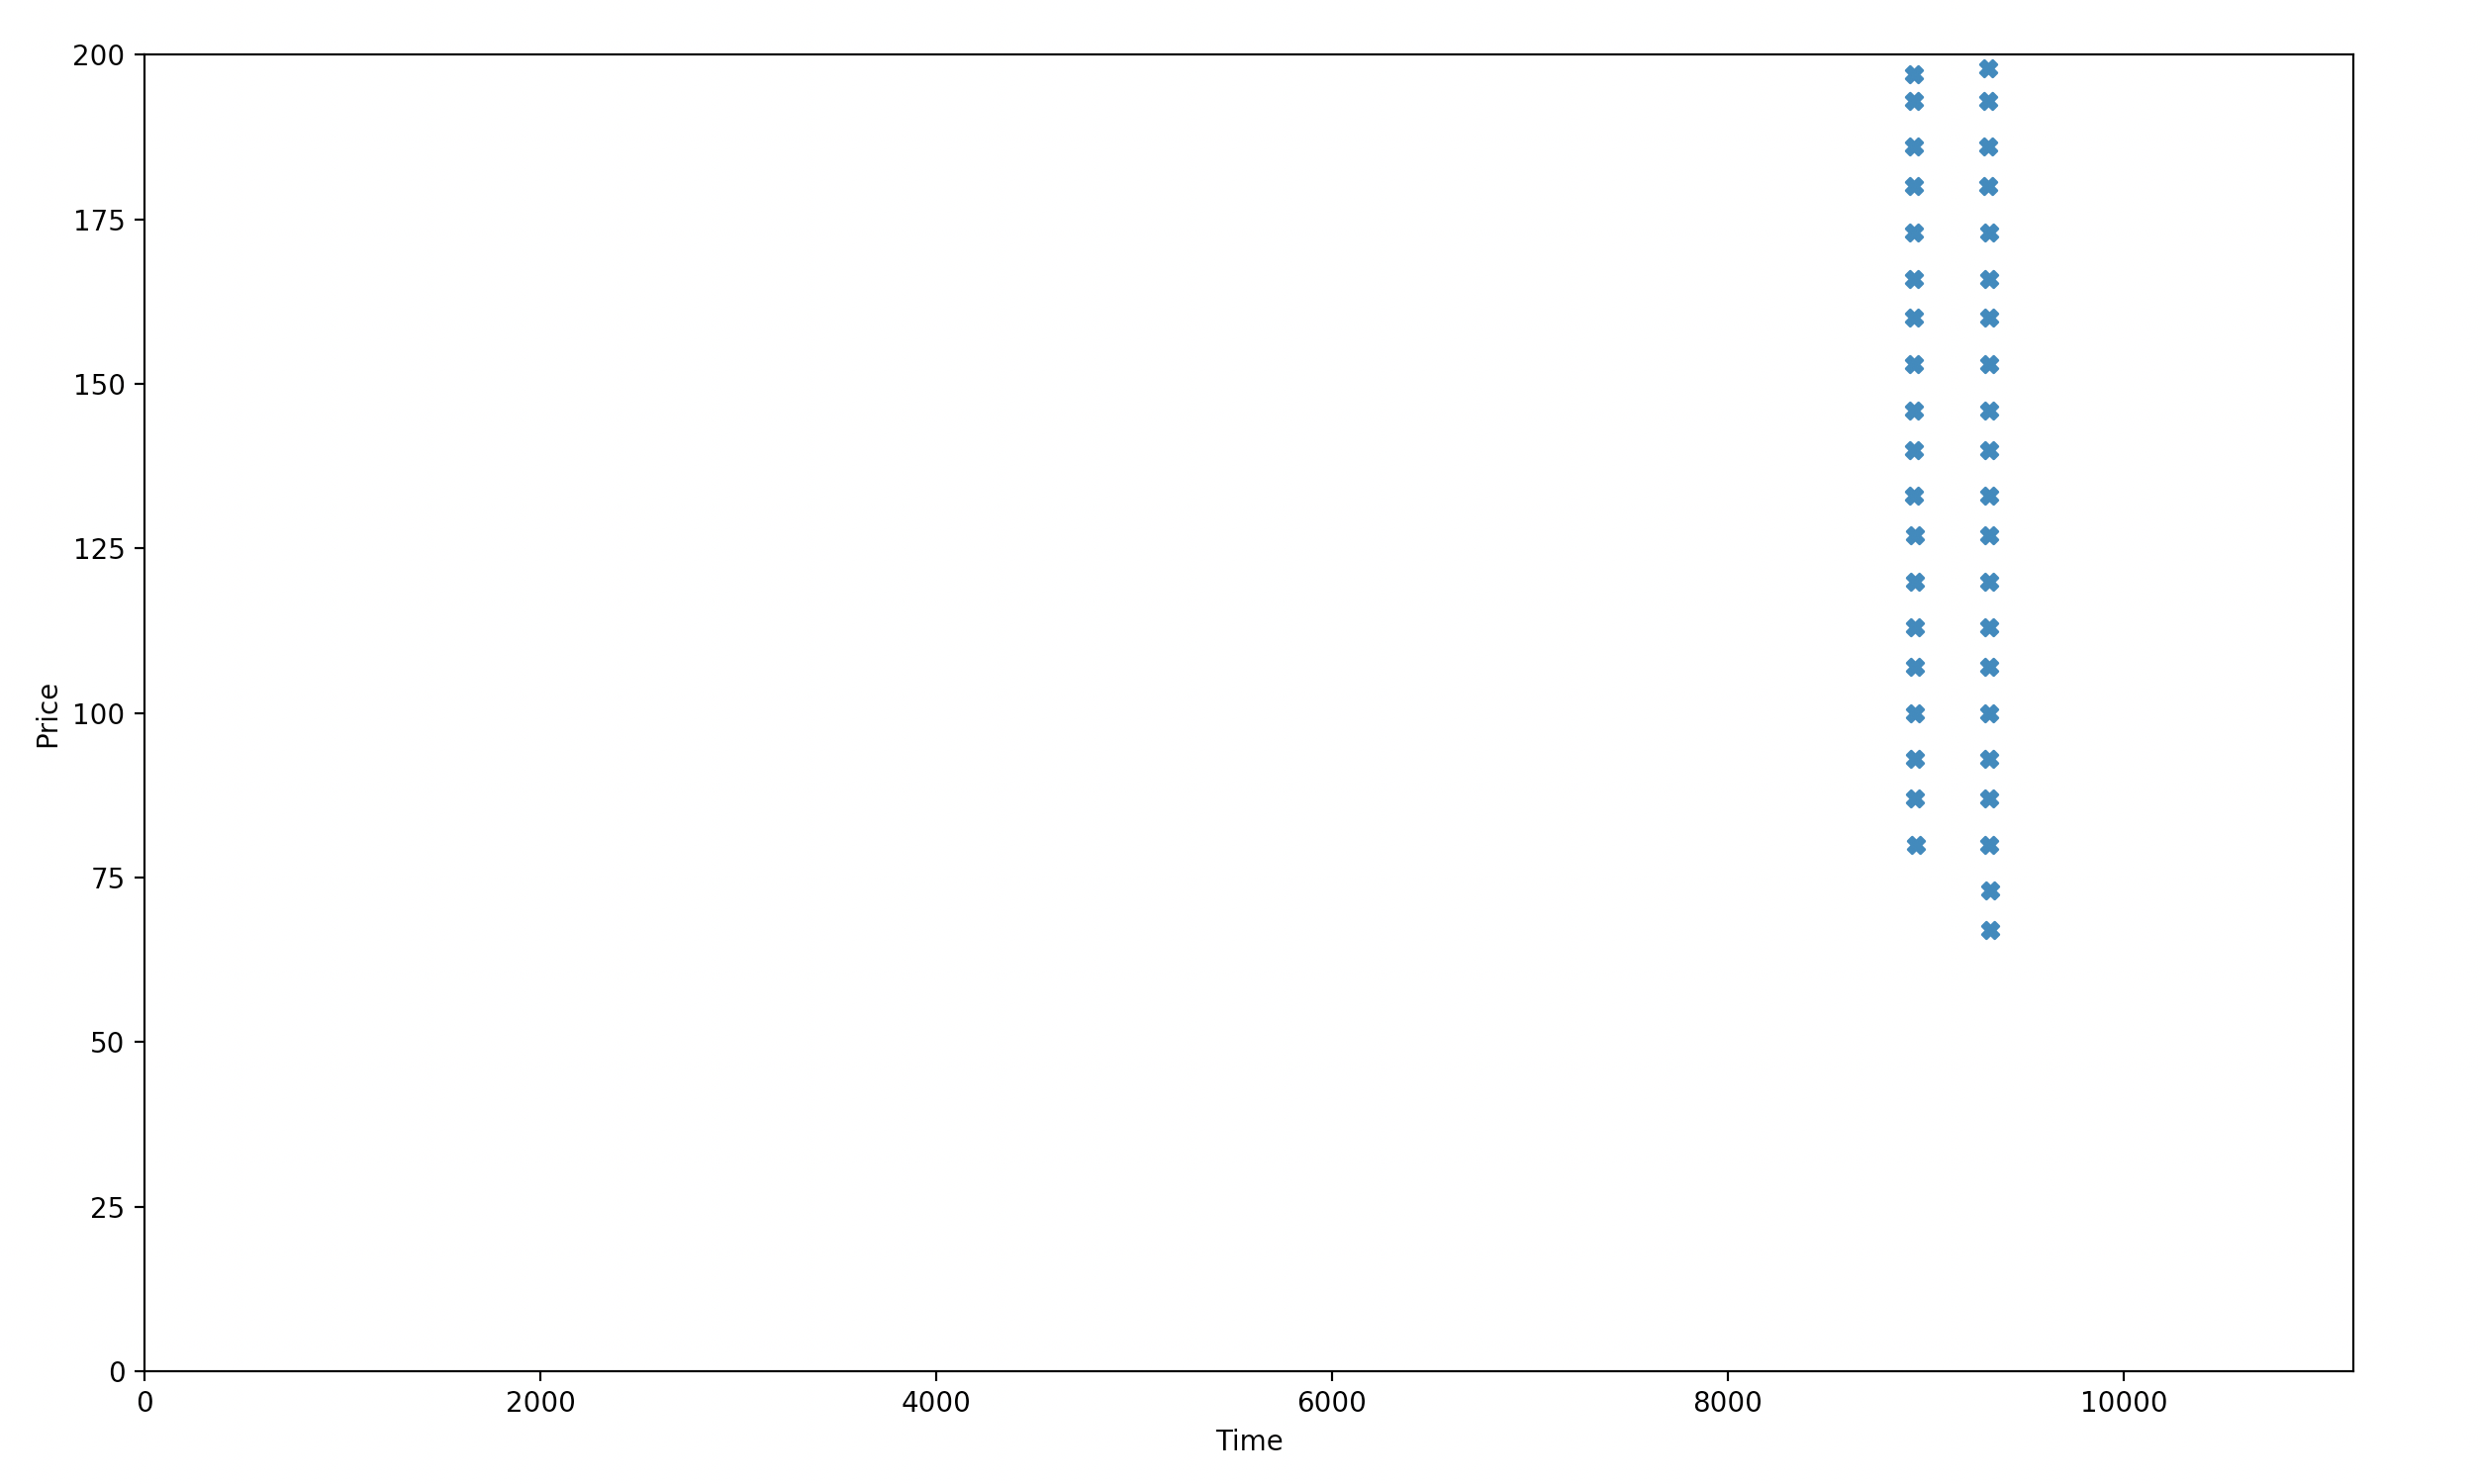
\includegraphics[ height=8cm]{Dissertation/images/snpr_adapted/2lines.png}
\caption{62 Sniper agents homogeneous market transaction diagram with 100 price equilibrium from complex order types implementation} 
\label{fig:sniper_wrong}
\end{figure} 
\FloatBarrier

After reducing the lurk threshold from 0.2 to 0.1, the agent behaviour now matches the base line results. 

\begin{figure}[h]
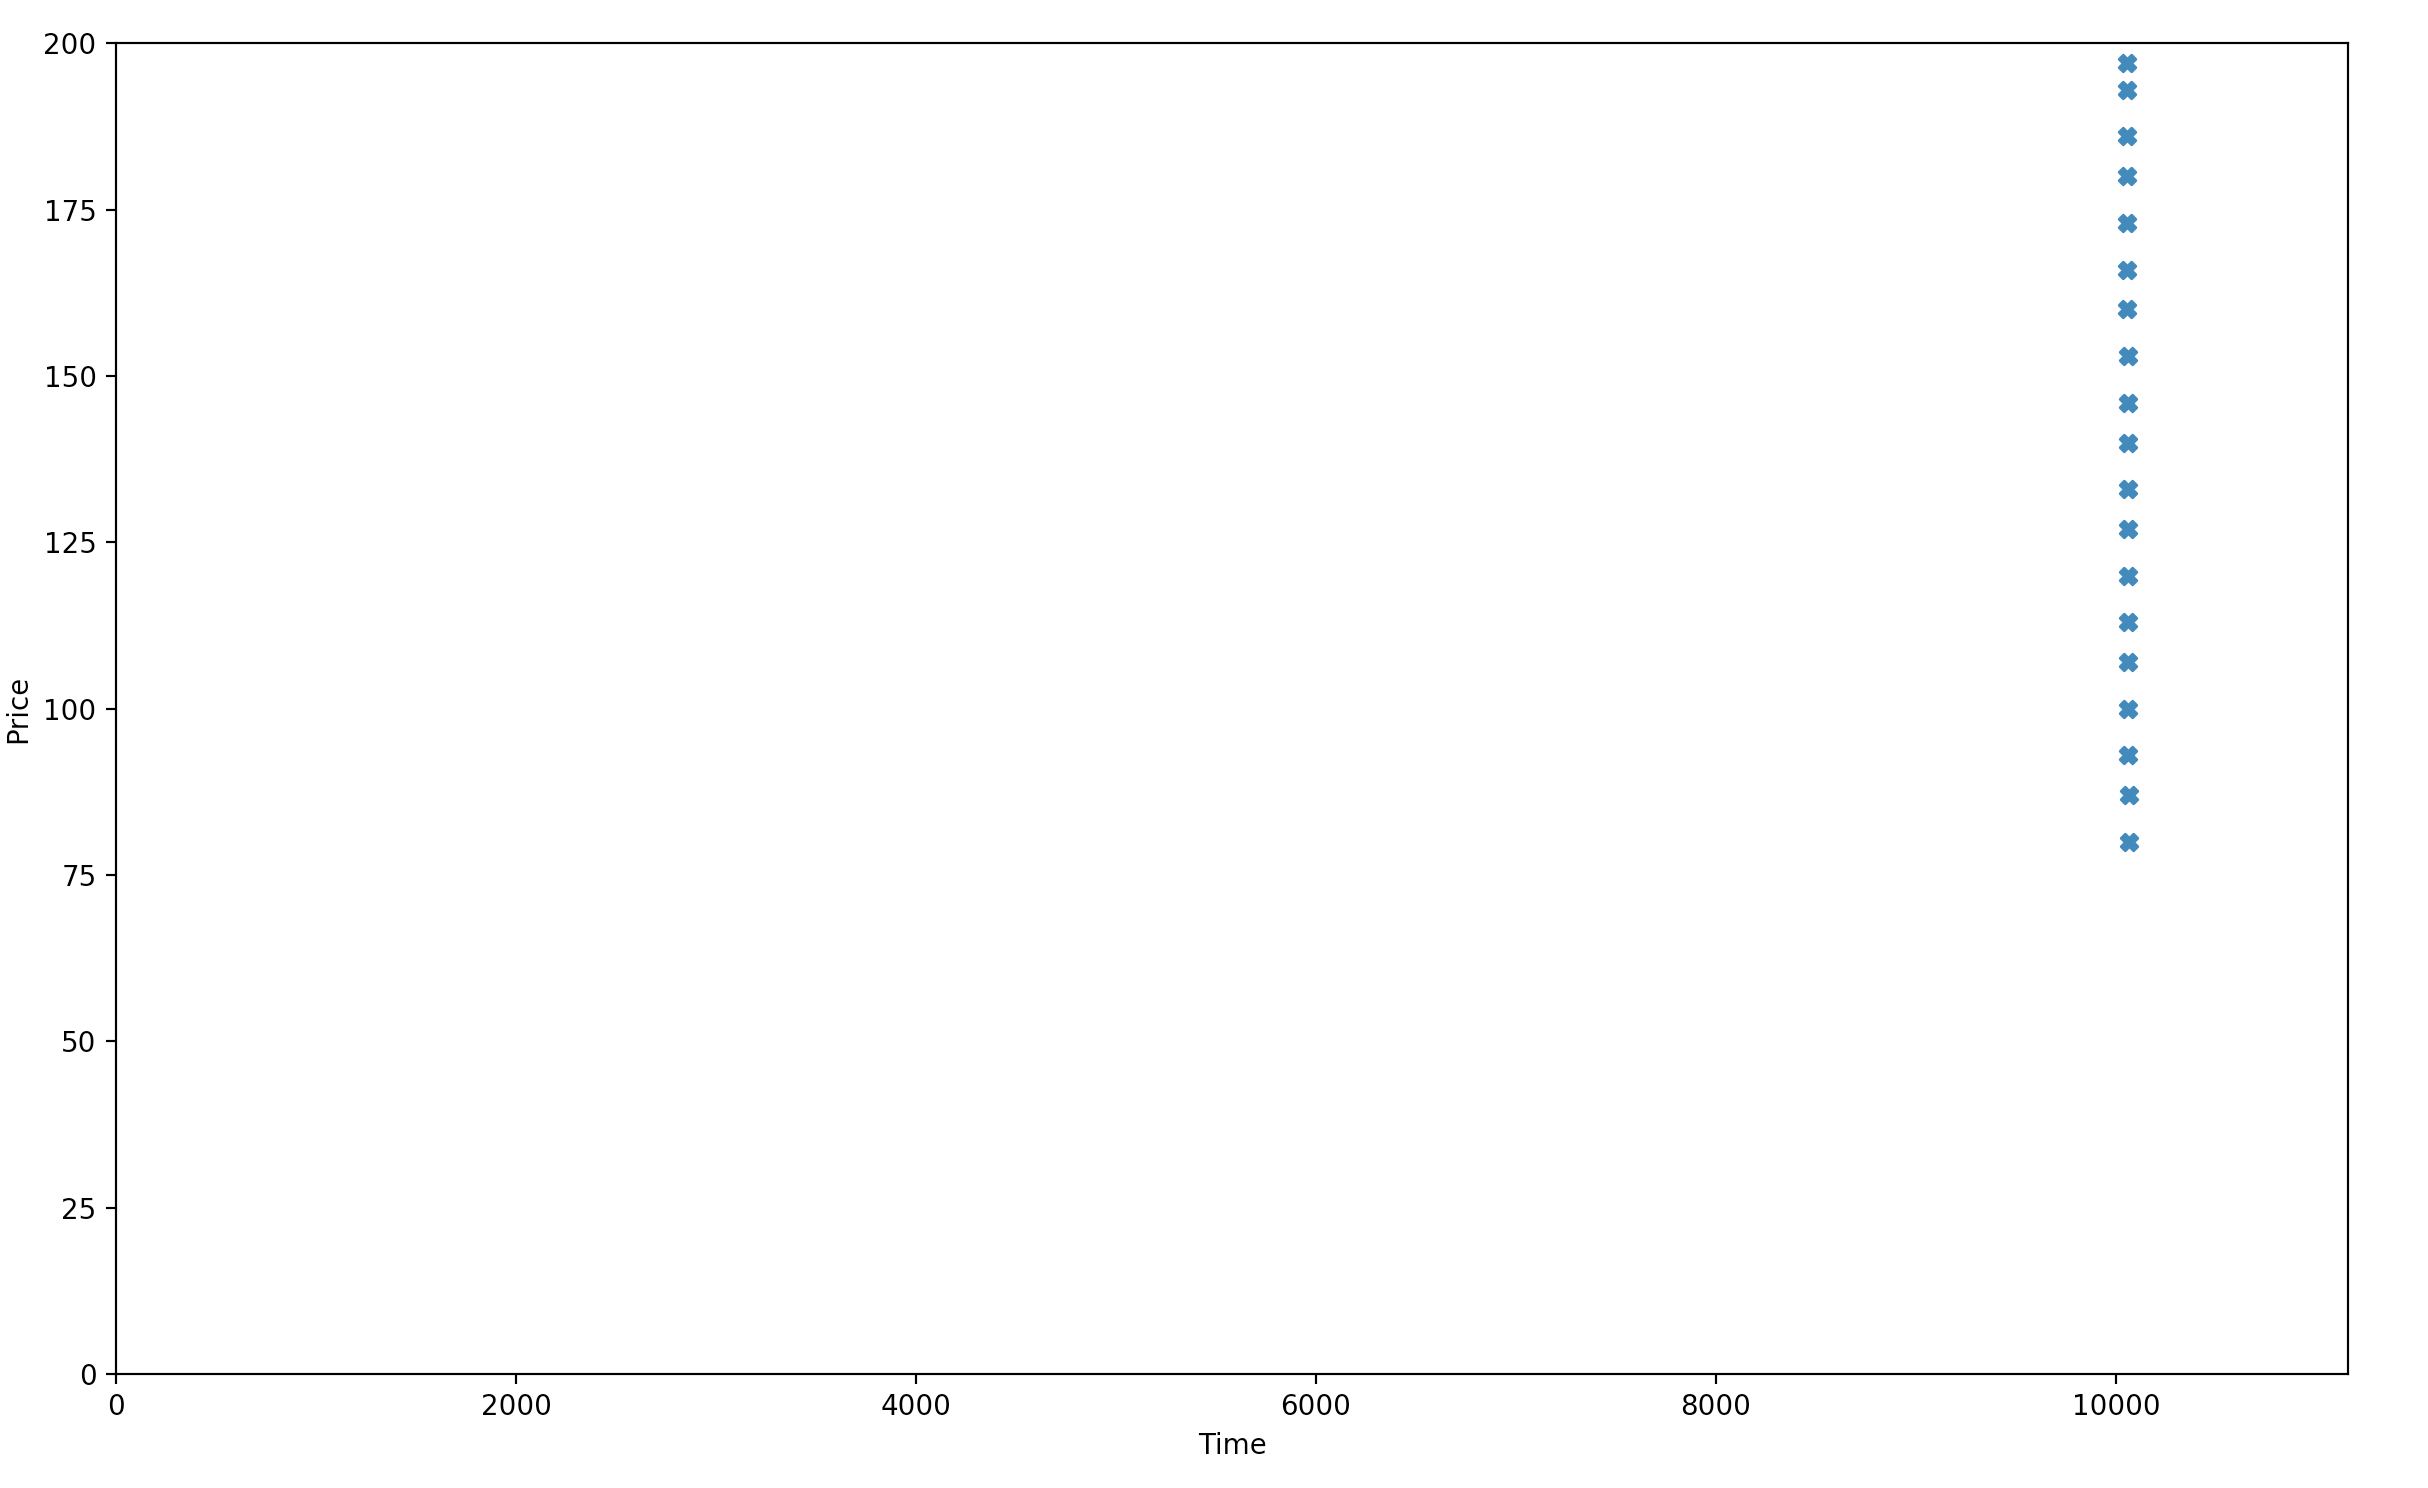
\includegraphics[ height=8cm]{Dissertation/images/snpr_adapted/adapted.png}
\caption{Adapted Sniper agent with Lurk threshold = 0.1}
\label{fig:SNIPER_FINAL}
\end{figure} 
\FloatBarrier

\begin{figure}[h]
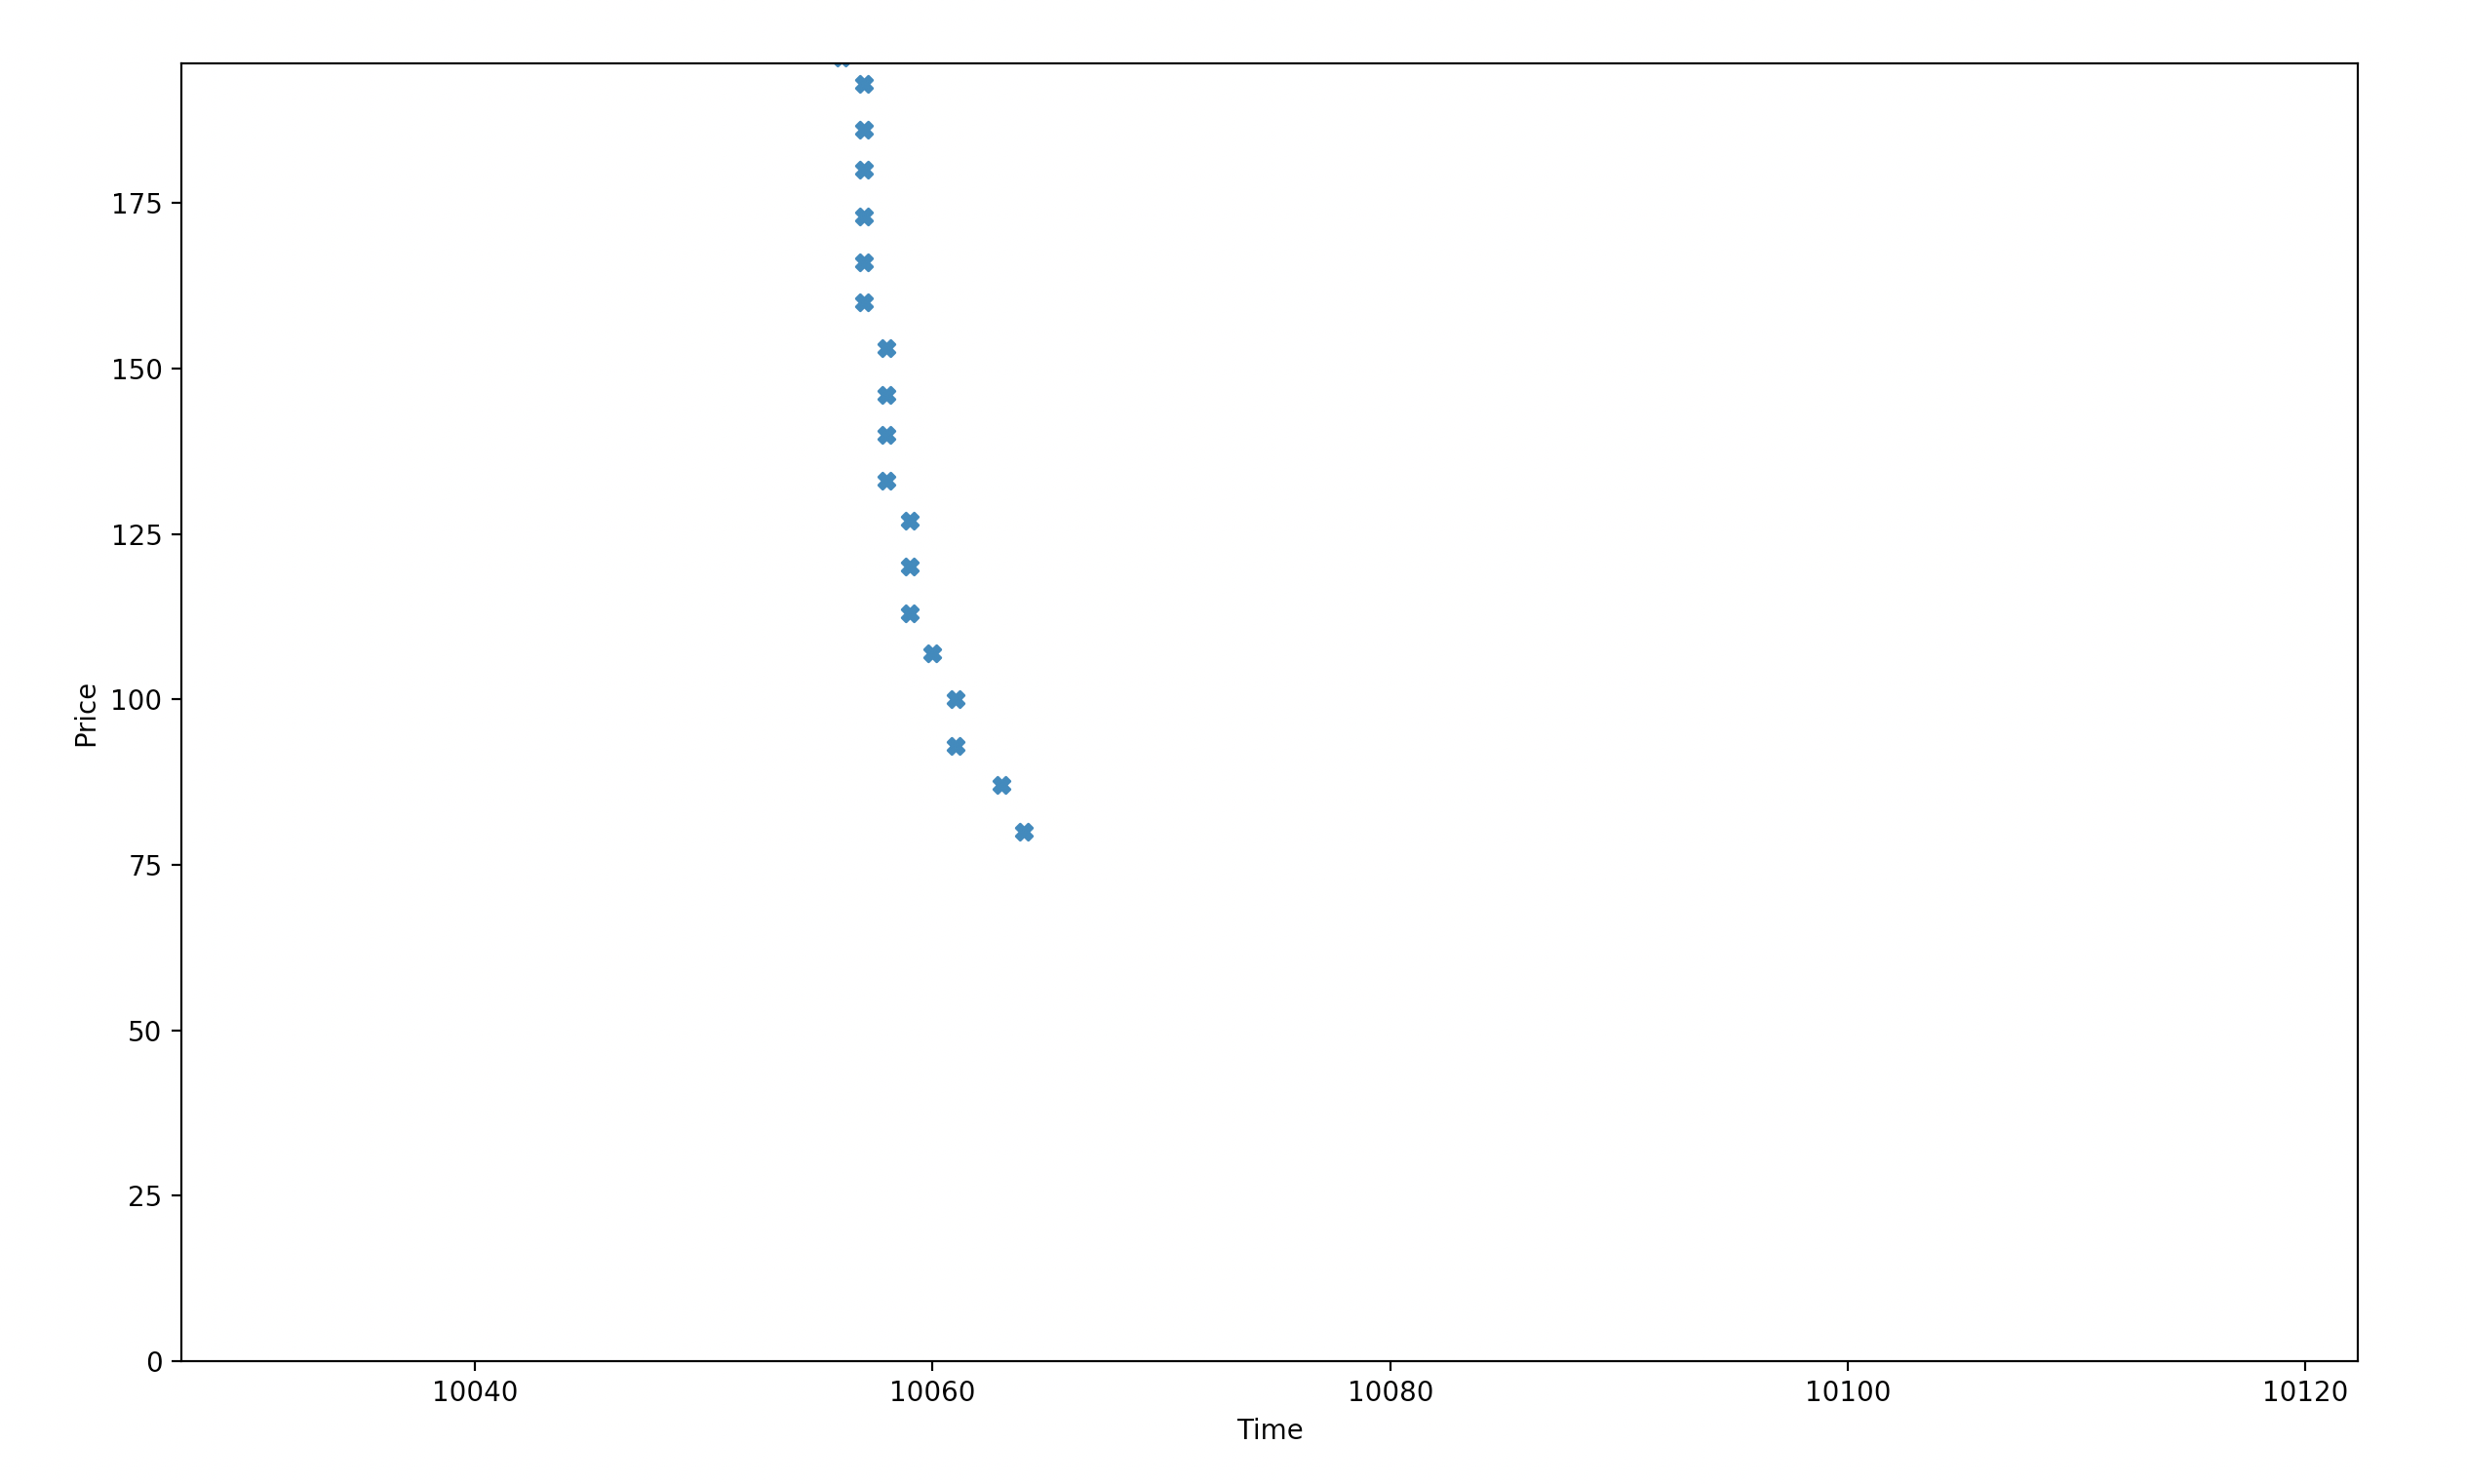
\includegraphics[ height=8cm]{Dissertation/images/snpr_adapted/zoom.png}
\caption{Zoomed-in graph of the Figure \ref{fig:SNIPER_FINAL}} 
\end{figure} 
\FloatBarrier

\subsection{ZI-C}
ZIC's behaviour in the new LOB is still similar to the one ran in the original BSE. The transaction price does not converge in any period of the session.

\begin{figure}[h]
\includegraphics[ height=8cm]{Dissertation/images/change2/zic.png}
\caption{62 ZI-C agents homogeneous market transaction diagram with 100 price equilibrium from McG action step implementation}  
\end{figure} 
\FloatBarrier

\subsection{ZI-P}
In ZIP's case, the implementation and adaptation is much more complex. In the experiment, the results suggest that the probability of acting for ZI-P agent (implemented so that it is similar to the McG agents) play a huge role in the convergence of ZI-P equilibrium. The parameter $p_{zip}$ is the probability of acting of the ZI-P agent. The adaptation is very similar to how McG adapted the Oesch's agents (Market maker and Liquidity consumer) to their model in which the Oesch's \cite{Oesch} time system is very similar to that of BSE's. The Figure \ref{fig:ZIP_prob_all} illustrate the examples of ZI-P converge in each probability. It can clearly be seen that as the probability decreases, the convergence will be better. In the 1 case, the ZI-P barely converges at all. However, as the probability in 0.5 and 0.25, the transaction price slowly converges near the equilibrium at 100. 

\begin{figure}[h]
  \begin{subfigure}[b]{0.5\textwidth}
    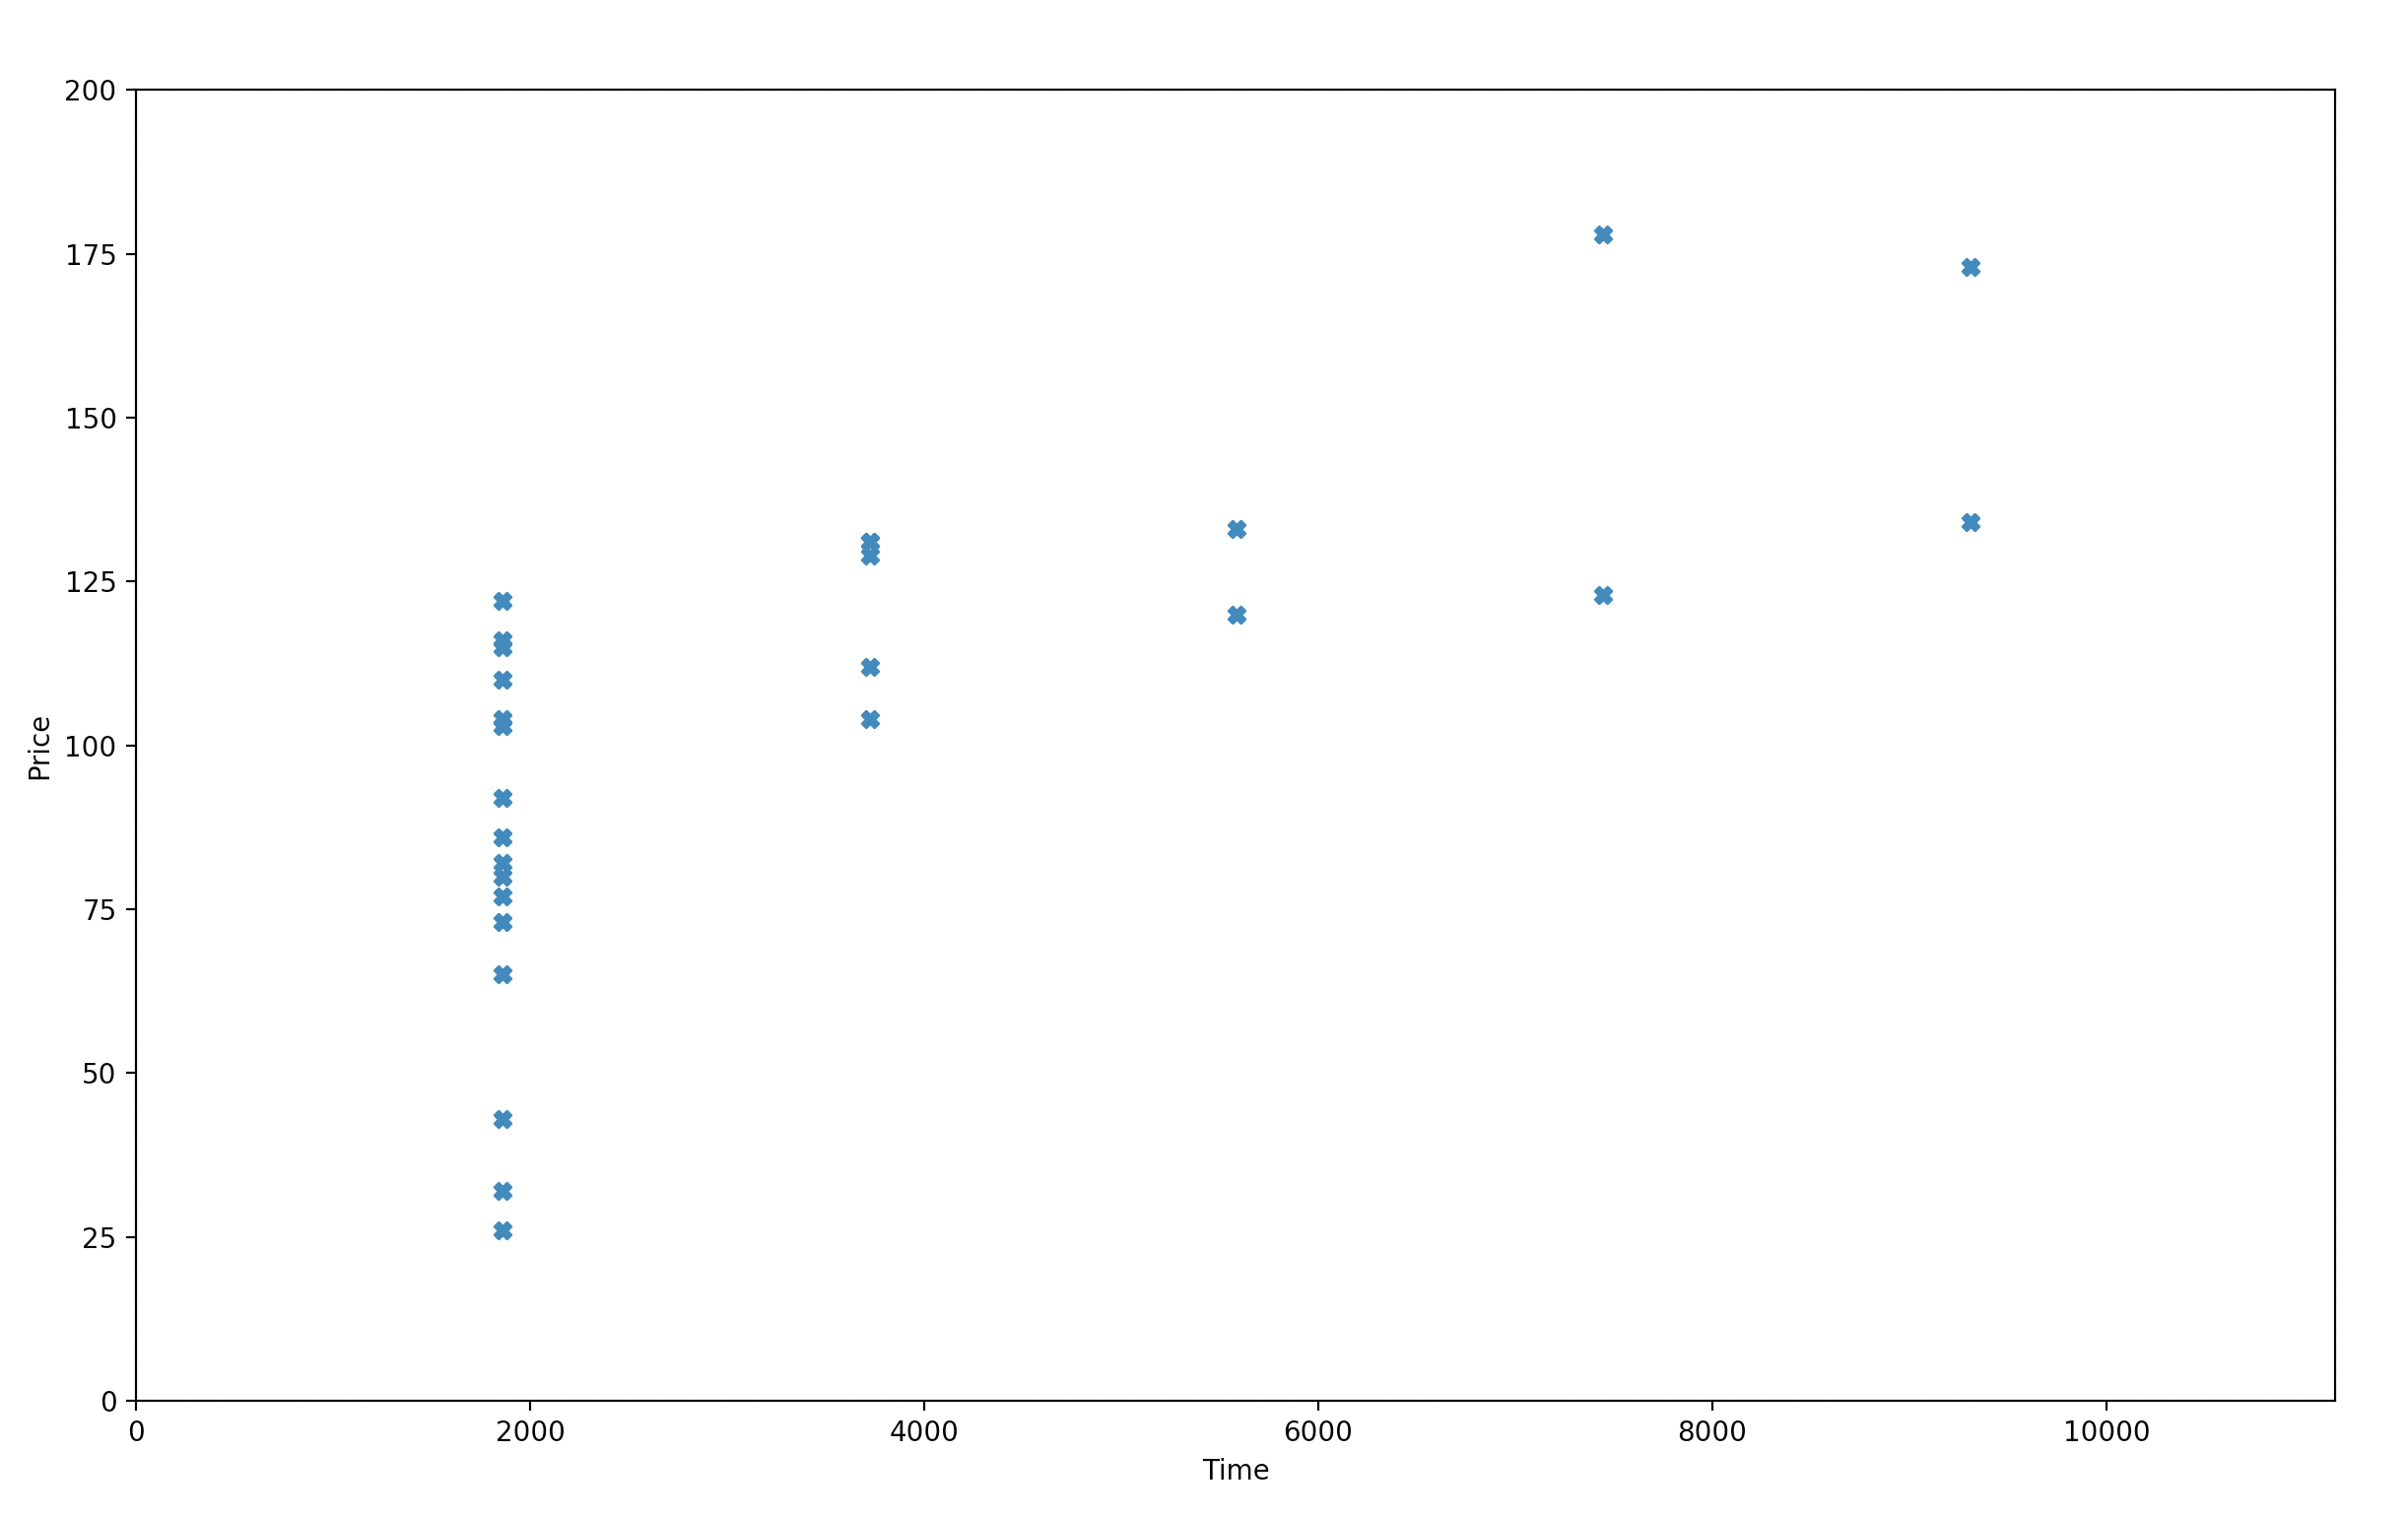
\includegraphics[width=7cm, height=7cm]{Dissertation/images/zip_randomized/1.png}
    \caption{ZI-P with $p_{zip} = 1$ }
    \label{fig:1}
  \end{subfigure}
  %
  \begin{subfigure}[b]{0.5\textwidth}
    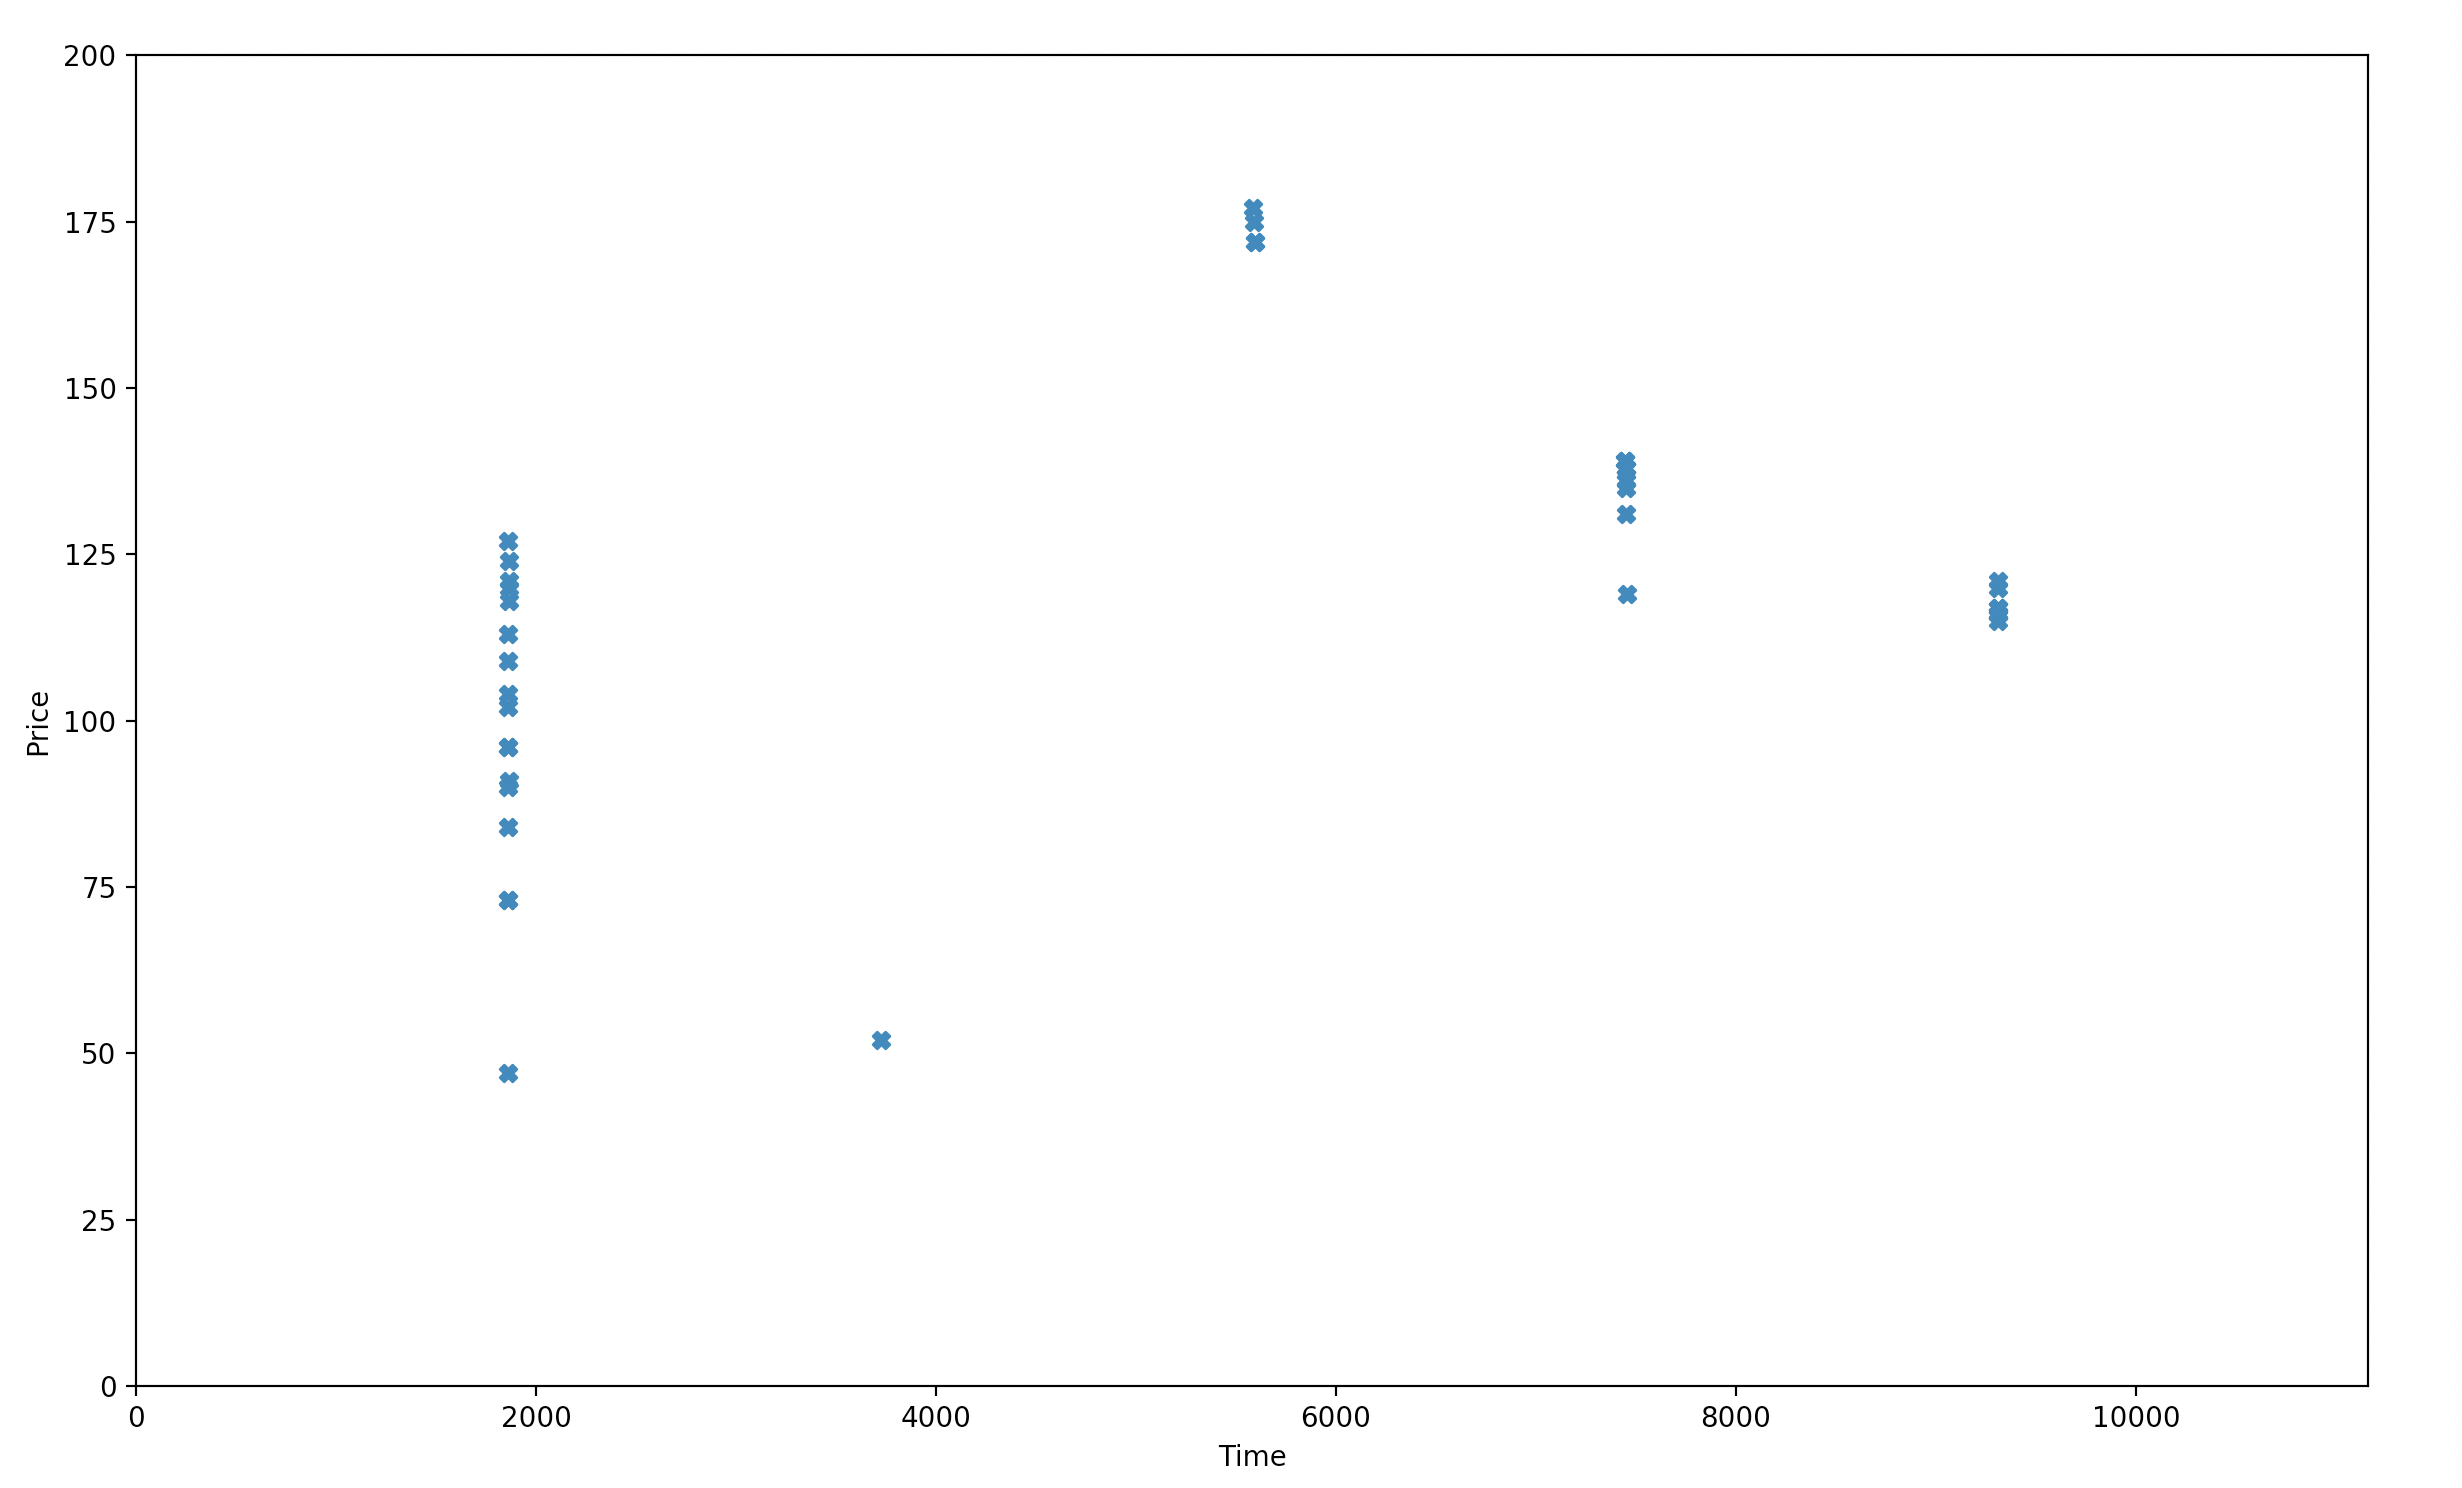
\includegraphics[width= 7cm, height=7cm]{Dissertation/images/zip_randomized/0.5.png}
    \caption{ZI-P with $p_{zip} = 0.5$}
    \label{fig:2}
  \end{subfigure}
\end{figure}

\begin{figure}[h]
  \begin{subfigure}[b]{0.5\textwidth}
    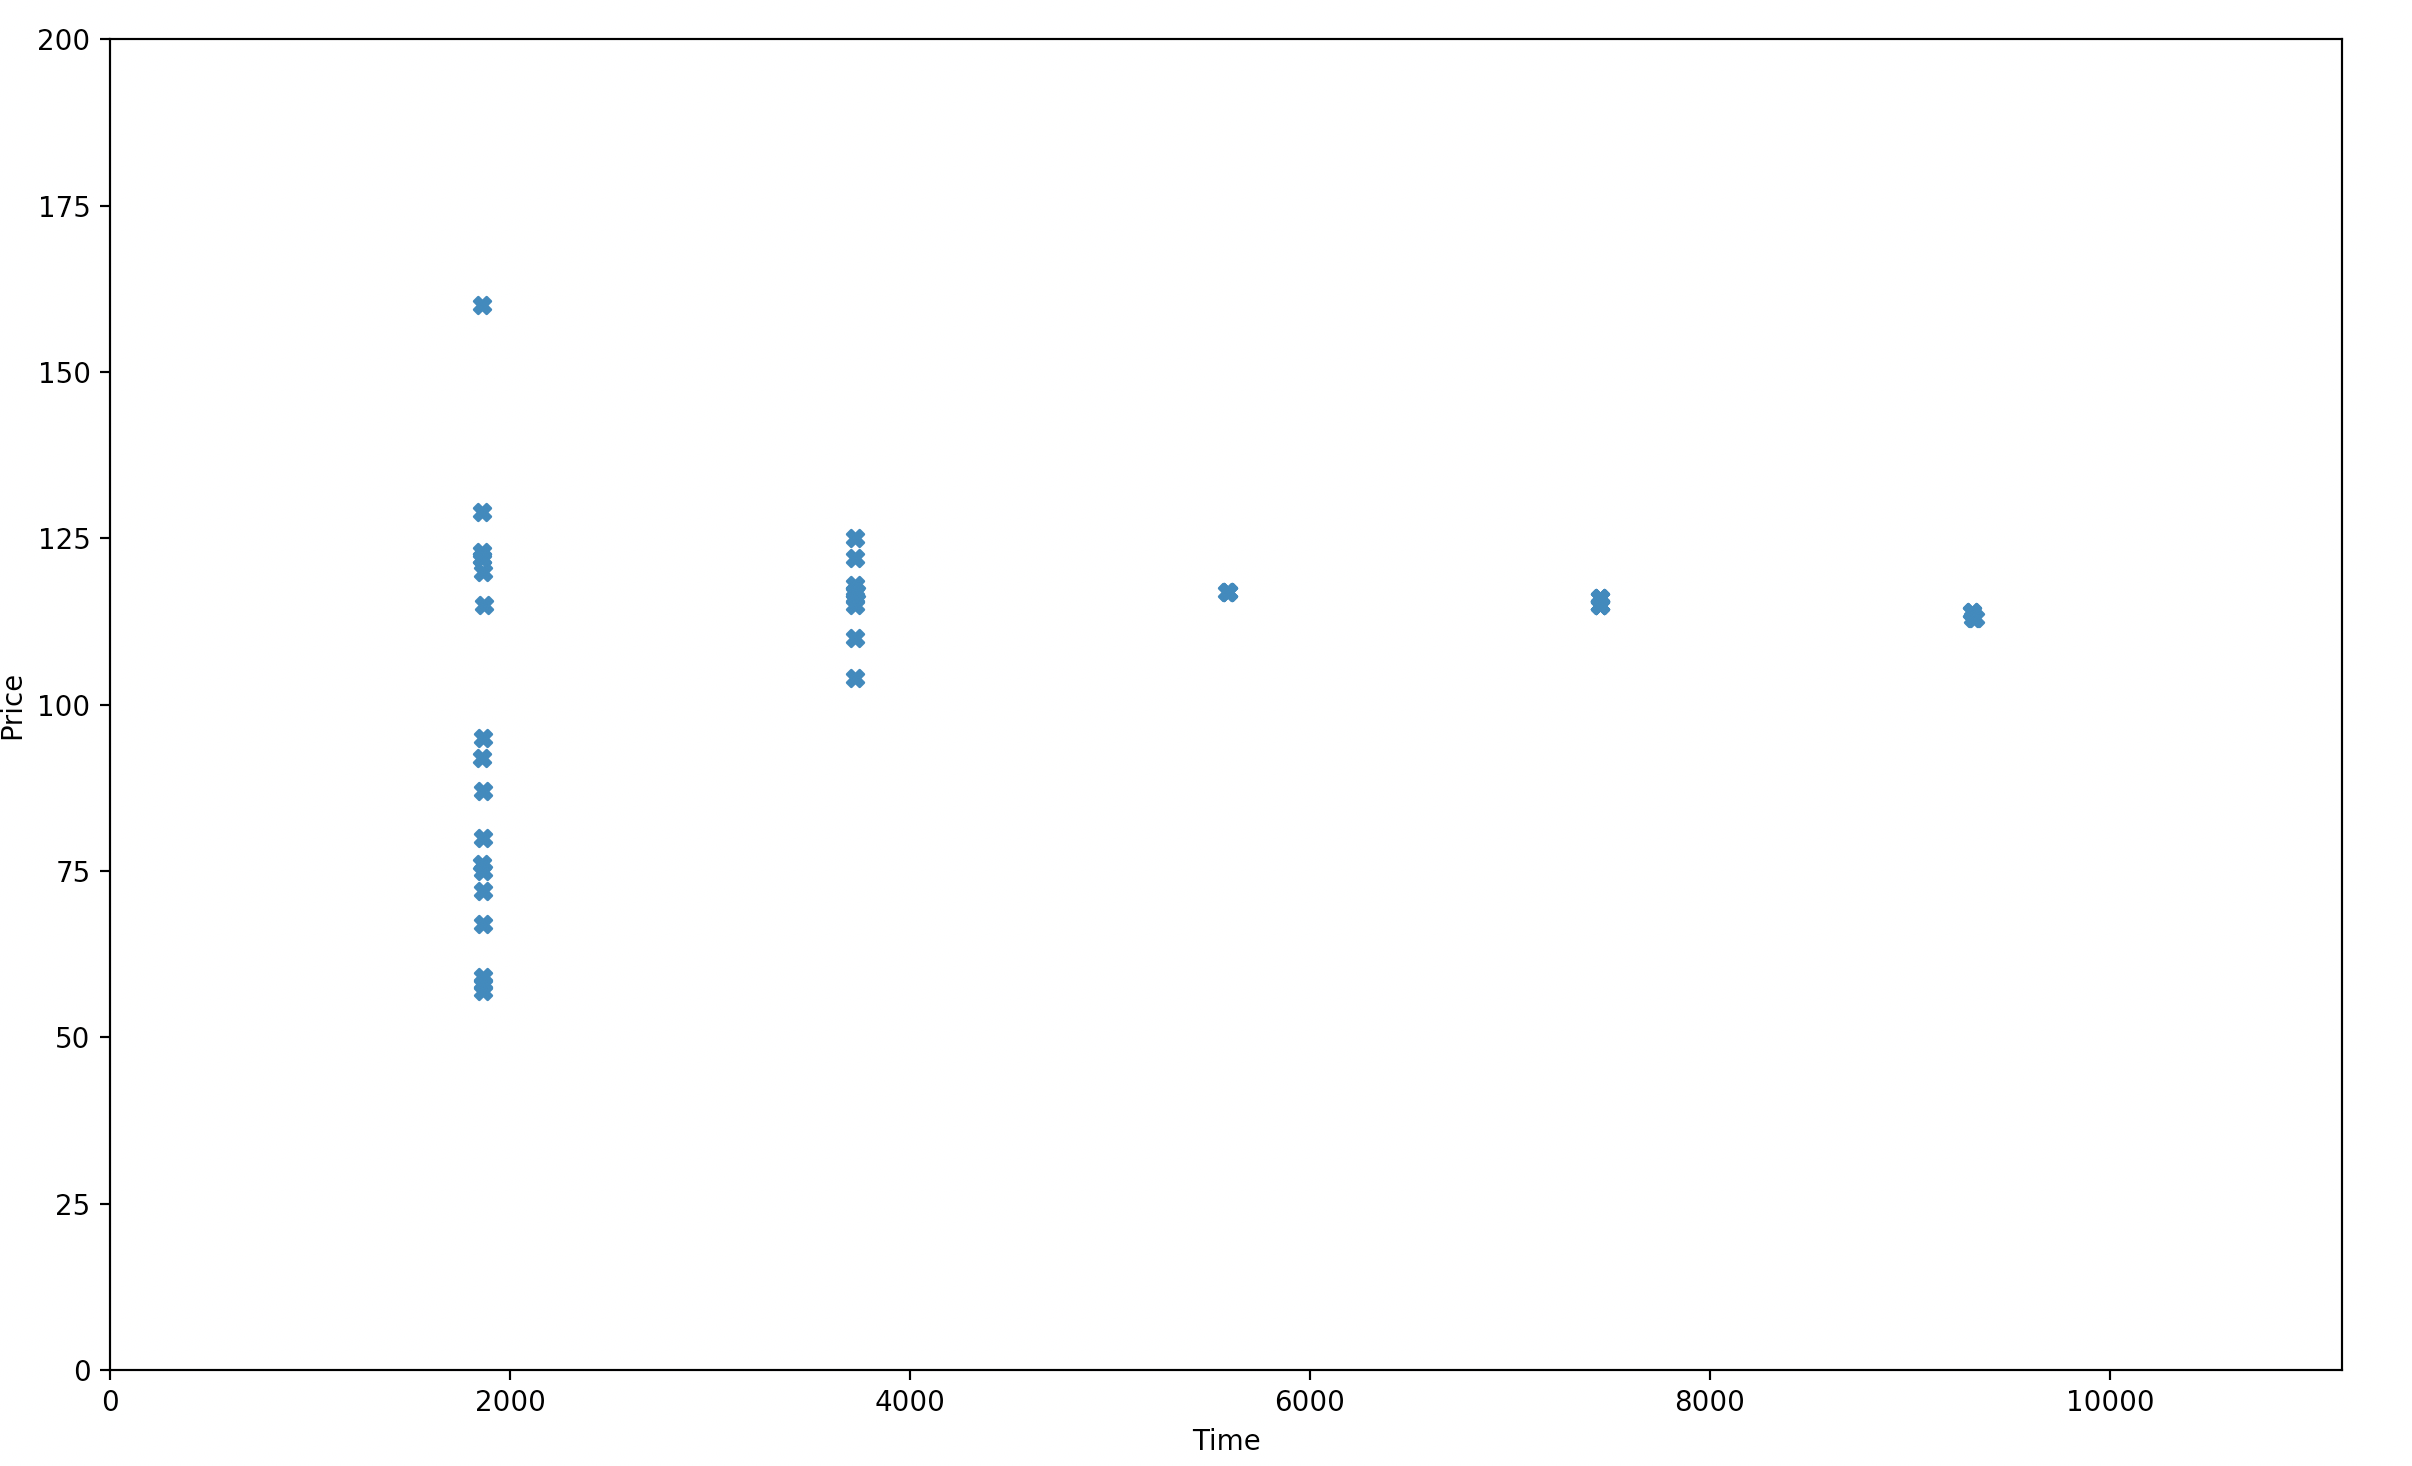
\includegraphics[width= 7cm, height=7cm]{Dissertation/images/zip_randomized/0.25.png}
    \caption{ZI-P with $p_{zip} = 0.25$}
    \label{fig:3}
  \end{subfigure}
  %
  \begin{subfigure}[b]{0.5\textwidth}
    \includegraphics[width= 7cm, height=7cm]{Dissertation/images/change2/zip.png}
    \caption{ZI-P with $p_{zip} = 0.1$}
    \label{fig:4}
  \end{subfigure}
\caption{Transaction diagrams of ZI-P with different probability of acting}
\label{fig:ZIP_prob_all}
\end{figure}

\begin{table}[h]
\centering
\begin{tabular}{ |m||p{4cm}|} 
\hline
\textbf{Probability}& \textbf{Smith's alpha value} \\
\hline
\hline
Original value & 24.8\\
\hline 
1 & 40.12 \\ 
\hline
0.5 & 41.12\\ 
\hline
0.25 & 32.0 \\ 
\hline
0.1 & 25.4 \\ 
\hline
\end{tabular}
\caption{Smith's alpha value after implementing probability of acting $p_{zip}$}  
\end{table}
\FloatBarrier
To illustrate this further, the figures below is the comparison between the final 0.1 probability with the original Base Line ZI-P behaviour. 

\begin{figure}[hbpt!]
  \begin{subfigure}[b]{0.5\textwidth}
    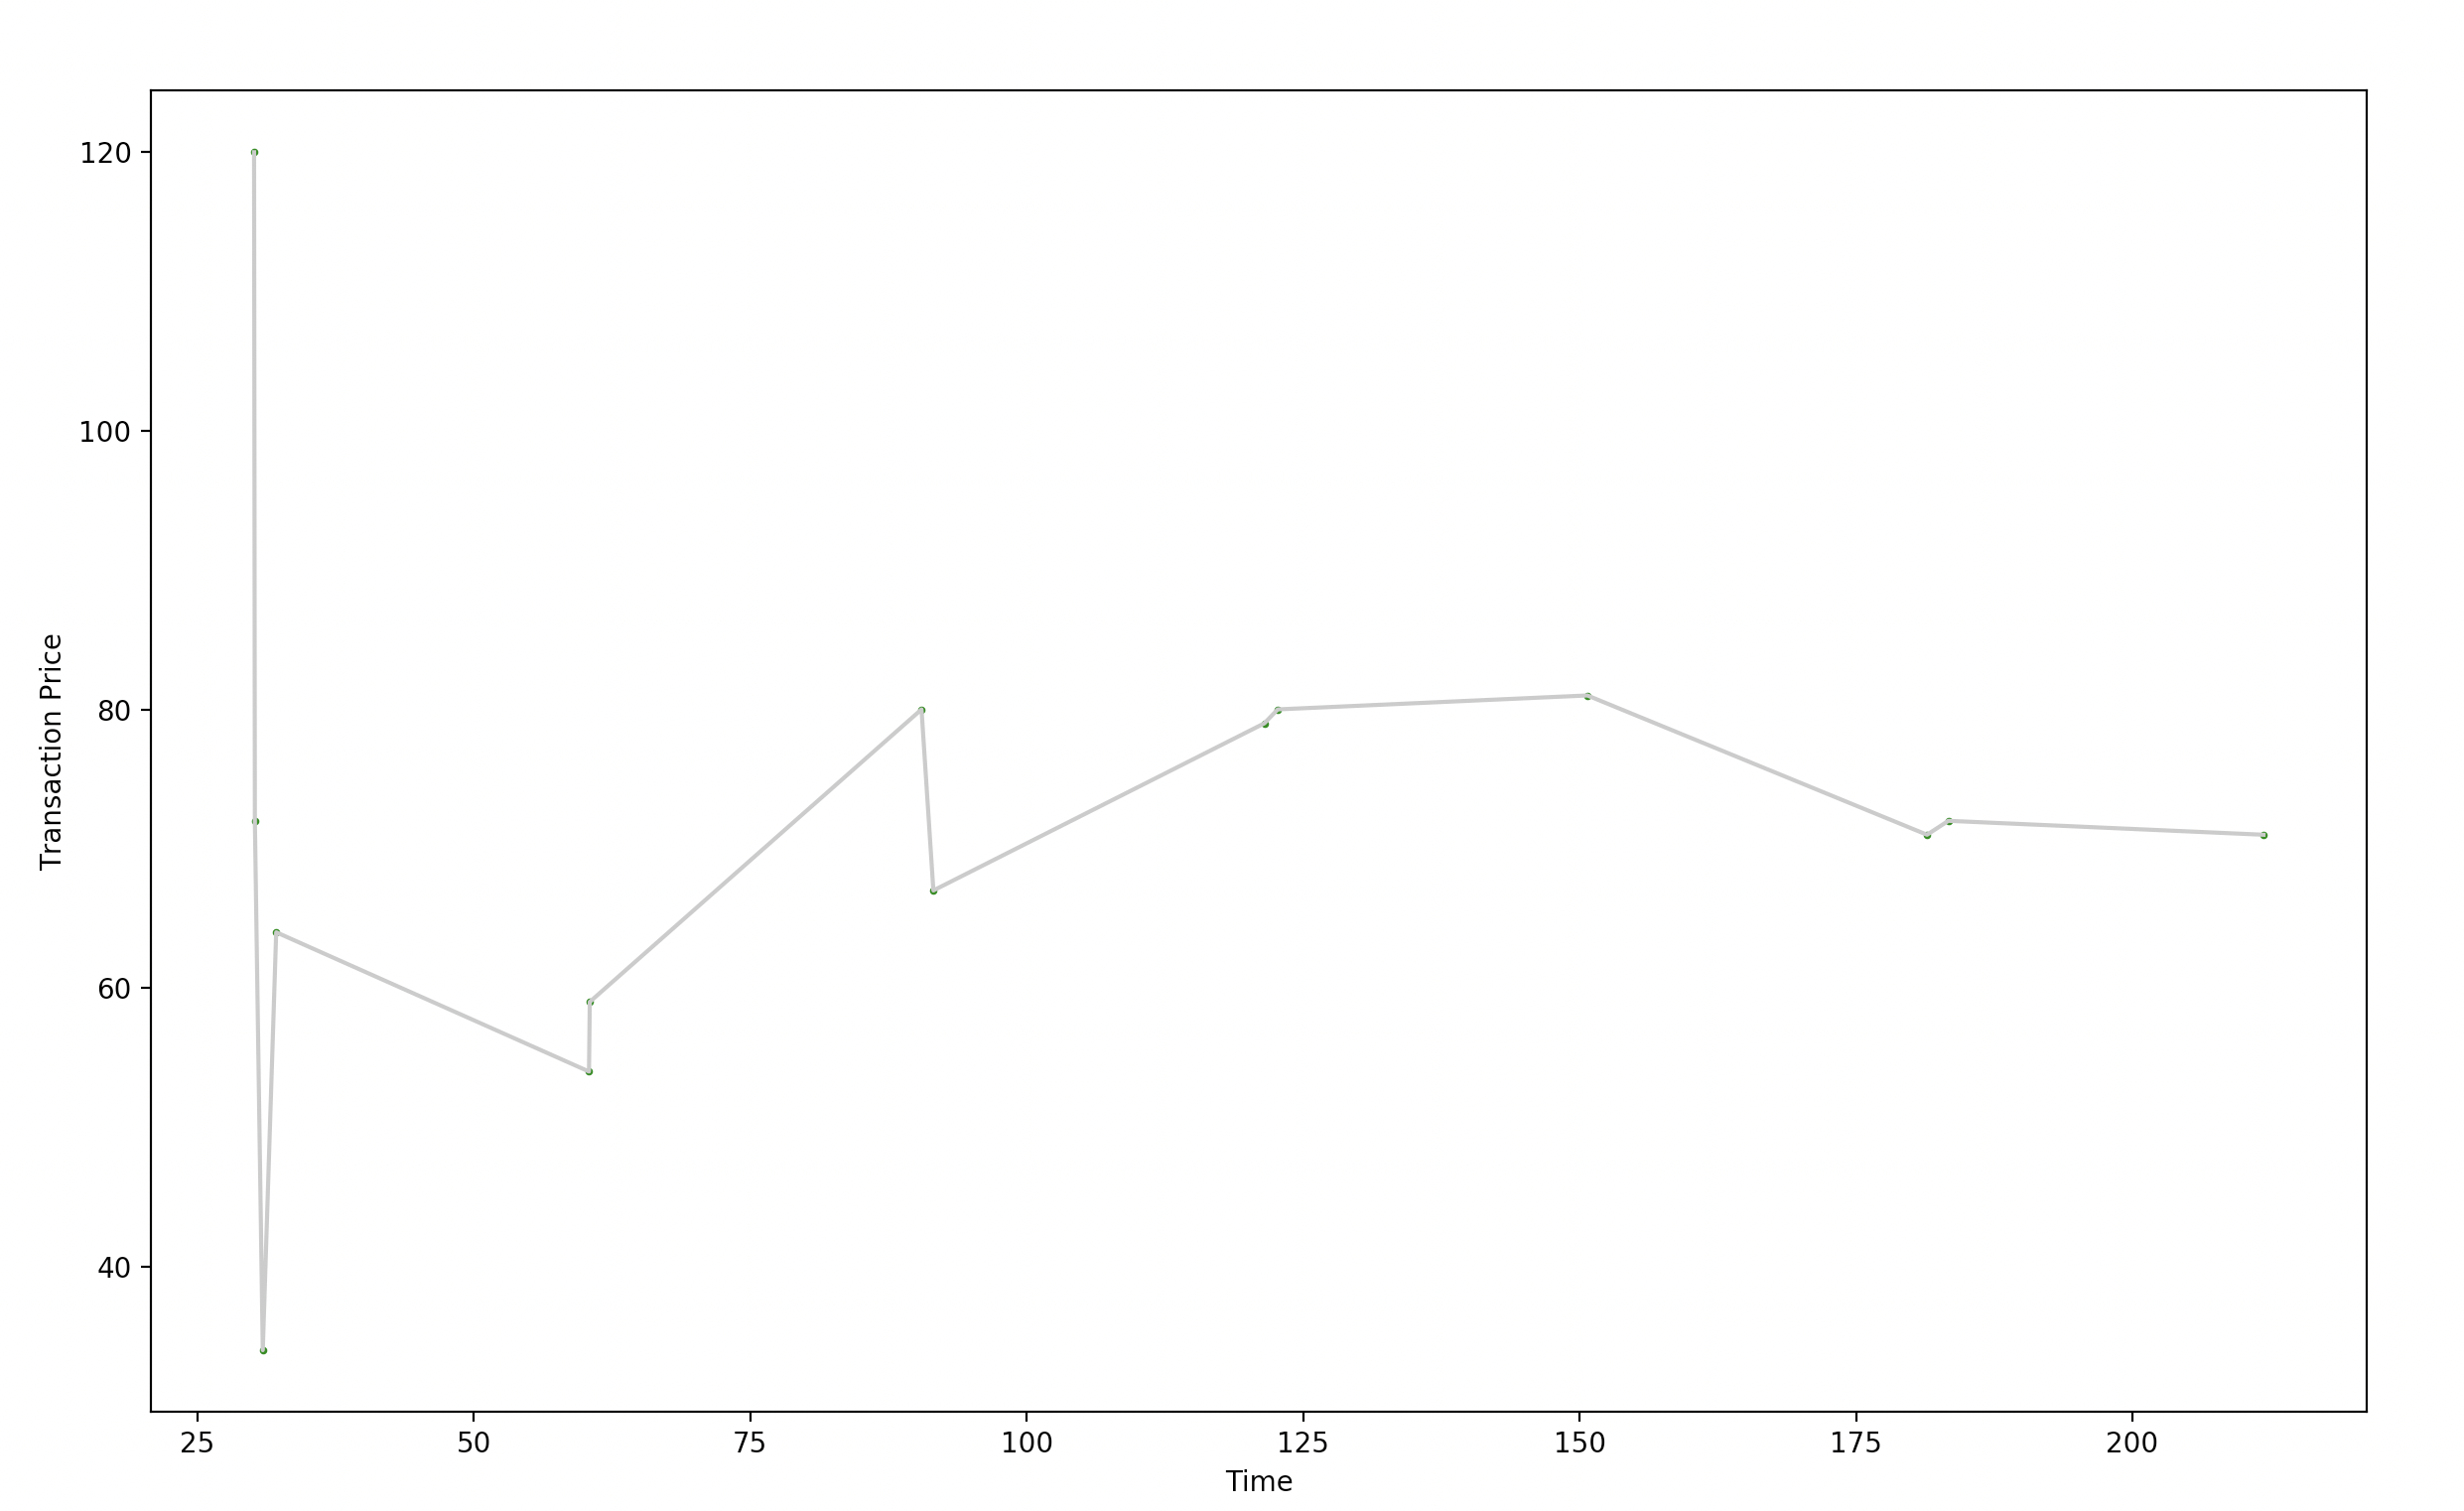
\includegraphics[ height=7cm, width = 7cm]{Dissertation/images/base_line/ZIP.png}
    \caption{Base Line ZI-P (same as Figure \ref{fig:ZIP_org_all}) }
    \label{fig:1}
  \end{subfigure}
  %
  \begin{subfigure}[b]{0.5\textwidth}
    \includegraphics[ height=7cm, width= 7cm]{Dissertation/images/change2/zip.png}
    \caption{ZI-P with $p_{zip} = 0.1$} 
    \label{fig:2}
  \end{subfigure}
\caption{Comparison of Base Line results of ZI-P and McG adapted parameter version} 
\end{figure}
\FloatBarrier

\section{Number of Transactions}
The table below illustrates the similarities of the number of transactions in each implementation of the BSE. As illustrated, the number of transactions in the market from the two new implementation versions are close to the original version of the BSE, hence is evidence that the agents are functioning properly. 

\begin{table}[h]
\centering
\begin{tabular}{ |m||p{4cm}|p{4cm}|p{4cm}|} 
\hline
\textbf{Agents}& \textbf{Base Line} & \textbf{Section 3.2 : Implemented Complex order types} & \textbf{Section 3.3: Implemented McG action step} \\
\hline
\hline
Kaplan's Sniper & 20 & 20 & 20 \\ 
\hline
ZI-C & 71 & 73 & 78\\ 
\hline
ZI-P & 42 & 45 & 47 \\ 
\hline
\end{tabular}
\caption{Number of transactions in each implementation}  
\end{table}
\FloatBarrier

\section{Evaluation}
This section's aim is to provide evidence that the market is function appropriately after implementing complex order types and McG action-steps. By evaluating the behaviours of the three existing agents : ZI-P, ZI-C and Sniper along with the Smith's alpha values, we can now established that the market is functional and stable. In the next chapter, we can now introduce new agents into the system. 

\chapter{McG Agents and their behaviour} 
Although McG paper does not clearly state any results of the agents individually, this thesis aims to investigate the integrity of the implementation. This will be done by examining the agents' algorithm in detail, along with the specific parameters in addition to looking at cited papers in McG which relates to where the McG's agents are based from. The aim of this section is to ensure that if the system (the new BSE) and the agents themselves are performing like what they are meant to do, we can be certain that any experiment results from the market consisting of the agents will be valid. 


\section{Market maker}
The Market maker in McG is modelled closely to Oesch 2014 conference paper \cite{Oesch}. Market makers are traders who attempt to earn a profit by taking advantage of the spread in the market. The agent executes orders on both bid and ask side of the LOB in each round. The agent submits a large order with volume $V=U(v_{min},v_{max})$ depending on its moving average. The moving average is used to predict what type of orders will be submitted next. 

\begin{algorithm}[H]
\DontPrintSemicolon 
\If{$random() > \delta_{mm}$} {
    Cancel any existing order\;
    \tcc{Condition 1}
    \If{predict next order is buy} {
    \tcc{$U(a,b)$  function represents value drawn uniformly between $a$ and $b$ }
    Submit sell at best price with volume $V=U(v_{min},v_{max})$\;
    Submit buy at best price with volume $V=v^{-}$\;
    }
    \tcc{Condition 2}
    \Else{
    Submit buy at best price with volume $V=U(v_{min},v_{max})$\;
    Submit sell at best price with volume $V=v^{-}$\;
    }
    \EndIf
  }
\EndIf
Update buy/sell prediction with w-period rolling mean\; 
\caption{{\sc Market maker reproduced from McG (4.1) \cite{McGroarty}} }
\label{algo:market_maker}
\end{algorithm}

\begin{table}[h]
\centering
\begin{tabular}{ |m||p{4cm}|} 
\hline
\textbf{Market maker Parameters}& \textbf{Value} \\
\hline
\hline
$v_{min}$ & 100 \\ 
\hline
$v_{max}$ & 200,000\\ 
\hline
$v^-$ & 1\\ 
\hline
$w$ & 50\\
\hline
\end{tabular}
\caption{Market maker trader parameters taken from \cite{McGroarty} and  \cite{Oesch}} 
\end{table}
\FloatBarrier 

To clarify, the Market maker will make its decision based on a moving average of $w$ period. The moving average is calculated from the number of bids and asks in the $w$ period. In McG, the paper refers to Long Term memory order flow such that the future order is heavily correlated with the orders in the past. In each period, a buy order is given a +1 and a sell -1. The sum of those, if is negative, the Market maker agent will predict that an ask order will arrive next. This means that the agent will submit a bid large order with best price and quantity uniformly distributed from $U(v_{min},v_{max})$ and an ask order with quantity = $v^-$. This is Condition 1 on line 3 of Algorithm \ref{algo:market_maker}. Vice versa, if the sum of the period is positive as outlined in Condition 2 on line 6 of Algorithm \ref{algo:market_maker}. 

In order to test the Market maker behaviour, two simpler agents is implemented called Simple Buyer and Simple Seller. The Simple Buyer (Seller) will only submit a bid (an ask) order with price = $100$ in any circumstances with quantity uniformly distributed between 1 and 100. The total time period is 100 running with McG action step system. A short experiment is conducted where a market consisting of 6 Market makers and 6 of one of the Simple agents. The expected behaviour is that the Market maker will submit only an Ask order in a market with Simple Buyer since it will try to match the incoming bid orders. This is testing the first condition of the Algorithm \ref{algo:market_maker} where the Market maker will predict the next order is a buy. Vice versa for a market with Simple Seller. 

\begin{figure}[h]
  \begin{subfigure}[b]{0.5\textwidth}
    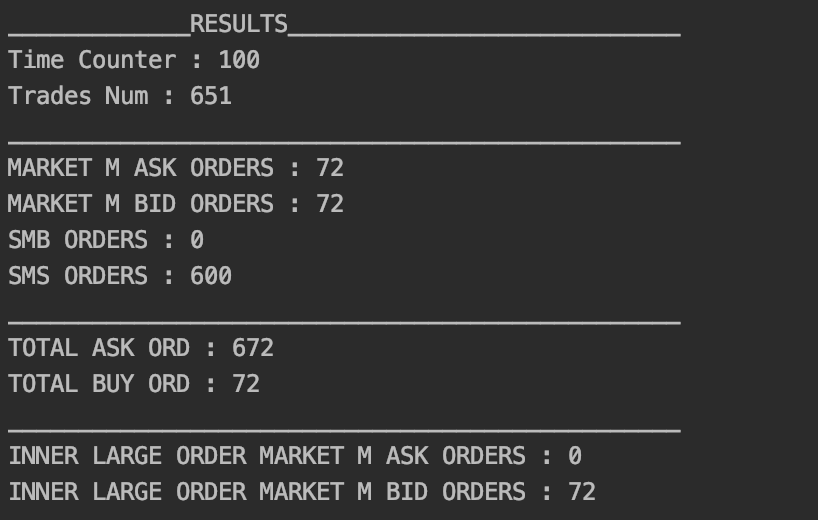
\includegraphics[width=7cm, height=6cm]{Dissertation/images/mcg_indv/SMS.png}
    \caption{Market maker with Simple Seller}
    \label{fig:indv_mm_1}
  \end{subfigure}
  %
  \begin{subfigure}[b]{0.5\textwidth}
    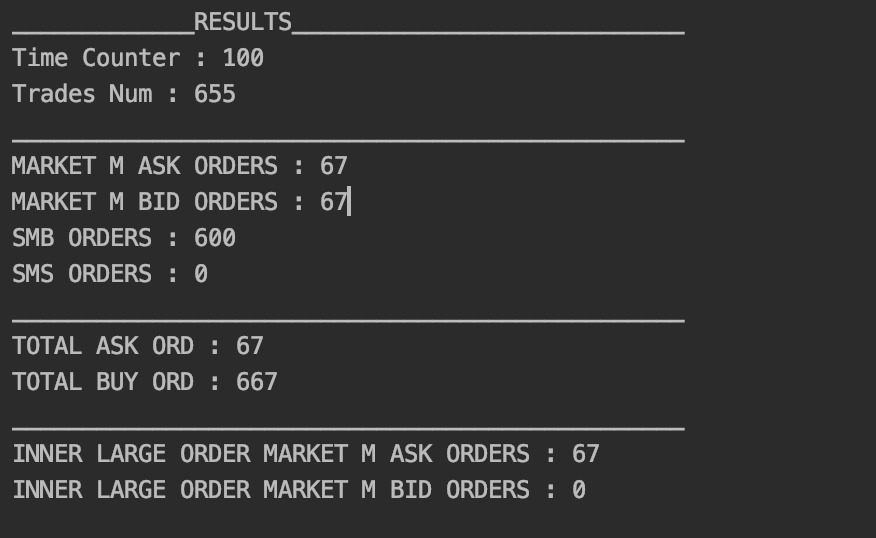
\includegraphics[width= 7cm, height=6cm]{Dissertation/images/mcg_indv/SMB.png}
    \caption{Market maker with Simple Buyer}
    \label{fig:indv_mm_2}
  \end{subfigure}
\caption{Market maker with Simple agent statistics} 
\end{figure}
\FloatBarrier

In Figure \ref{fig:indv_mm_1}, it can be seen that the bid large order of the Market maker is the only one submitted (72 submitted). This is because all of the orders in the Market submitted by the Simple Seller is an ask order. This means that only Condition 1 of Algorithm \ref{algo:market_maker} will be executed.  In addition, the number of total asks and bids submitted by the Market maker is also 72 because in each iteration, the Market maker submits both a bid and an ask order with the bid order at quantity $v^-$. 

Vice versa with Figure \ref{fig:indv_mm_2} where only ask large orders are submitted. This means that only Condition 2 of Algorithm \ref{algo:market_maker} will be executed because there are only bid orders submitted by the Simple Buyer agent.

\section{Liquidity consumer} 
In McG, the Liquidity consumer is also modelled closely to the Oesch 2014 \cite{Oesch} paper. Liquidity consumer represents large financial institution that makes trading decisions based on re-balancing the portfolio. At the start of the day, the agent decides, with equal probability, to sell or buy for the whole day. The Liquidity consumer will trade according to this large order, if empty, will generate a new one. In order to illustrate its behaviour, we adapted the Liquidity trader, only in this test, to draw an initial large order only once in the whole experiment. Note that by submitting market orders, only quantity is specified and not price since the market orders will execute at any price point until the quantity is fulfilled.  
\\
\begin{algorithm}[hbpt!]
\DontPrintSemicolon  
\If{start of the day} {
    \If{$random() > 0.5$} {
    Decides to Buy\;
    }
    \Else{
    Decides to Sell;\
    }
    \EndIf
    Initialize initial large order with volume $h_0 = U(h_{min},h_{max})$\;  
  }
\EndIf

\If{$random() < \delta_{lc}$} {
    \tcc{$\phi_t = $  the volume at the opposite best price at time t}
    \tcc{$h_t = $ is the remaining volume at time t}
    \tcc{Condition 1} 
    \If{$h_t \leq \phi_t$} {
    Submit market order with volume $v_t = h_t$\;
    }
    \tcc{Condition 2}
    \Else{
    Submit market order with volume $v_t = \phi_t$;\
    }
    \EndIf
    $h_t = h_t - v_t$\;  
  }
\EndIf
\caption{{\sc Liquidity consumer reproduced from McG (4.2) \cite{McGroarty} }}
\label{algo:liquidity_consumer}
\end{algorithm}

\begin{table}[h]
\centering
\begin{tabular}{ |m||p{4cm}|} 
\hline
\textbf{Liquidity consumer Parameters}& \textbf{Value} \\
\hline
\hline
$h_{min}$ & 1 \\ 
\hline
$h_{max}$ & 100,000\\ 
\hline
\end{tabular}
\caption{Liquidity consumer parameters taken from \cite{McGroarty} and  \cite{Oesch}} 
\end{table}
\FloatBarrier 

Because the Liquidity consumer only submits a market order, the only test that is viable is to see the quantity the agent has submitted. There are two cases that the quantity of a Liquidity trader will differ. The first case is when the best quantity of the opposite side is more than the remaining quantity and vice versa. The two tests below will demonstrate the agent's behaviour in both cases. Figures \ref{fig:liq_indv_1} and \ref{fig:liq_indv_1} illustrate the quantity of orders submitted in the whole market. The two tests consists of 6 Liquidity consumer and 6 Simple Seller. 

\begin{figure}[h]
  \begin{subfigure}[b]{0.5\textwidth}
    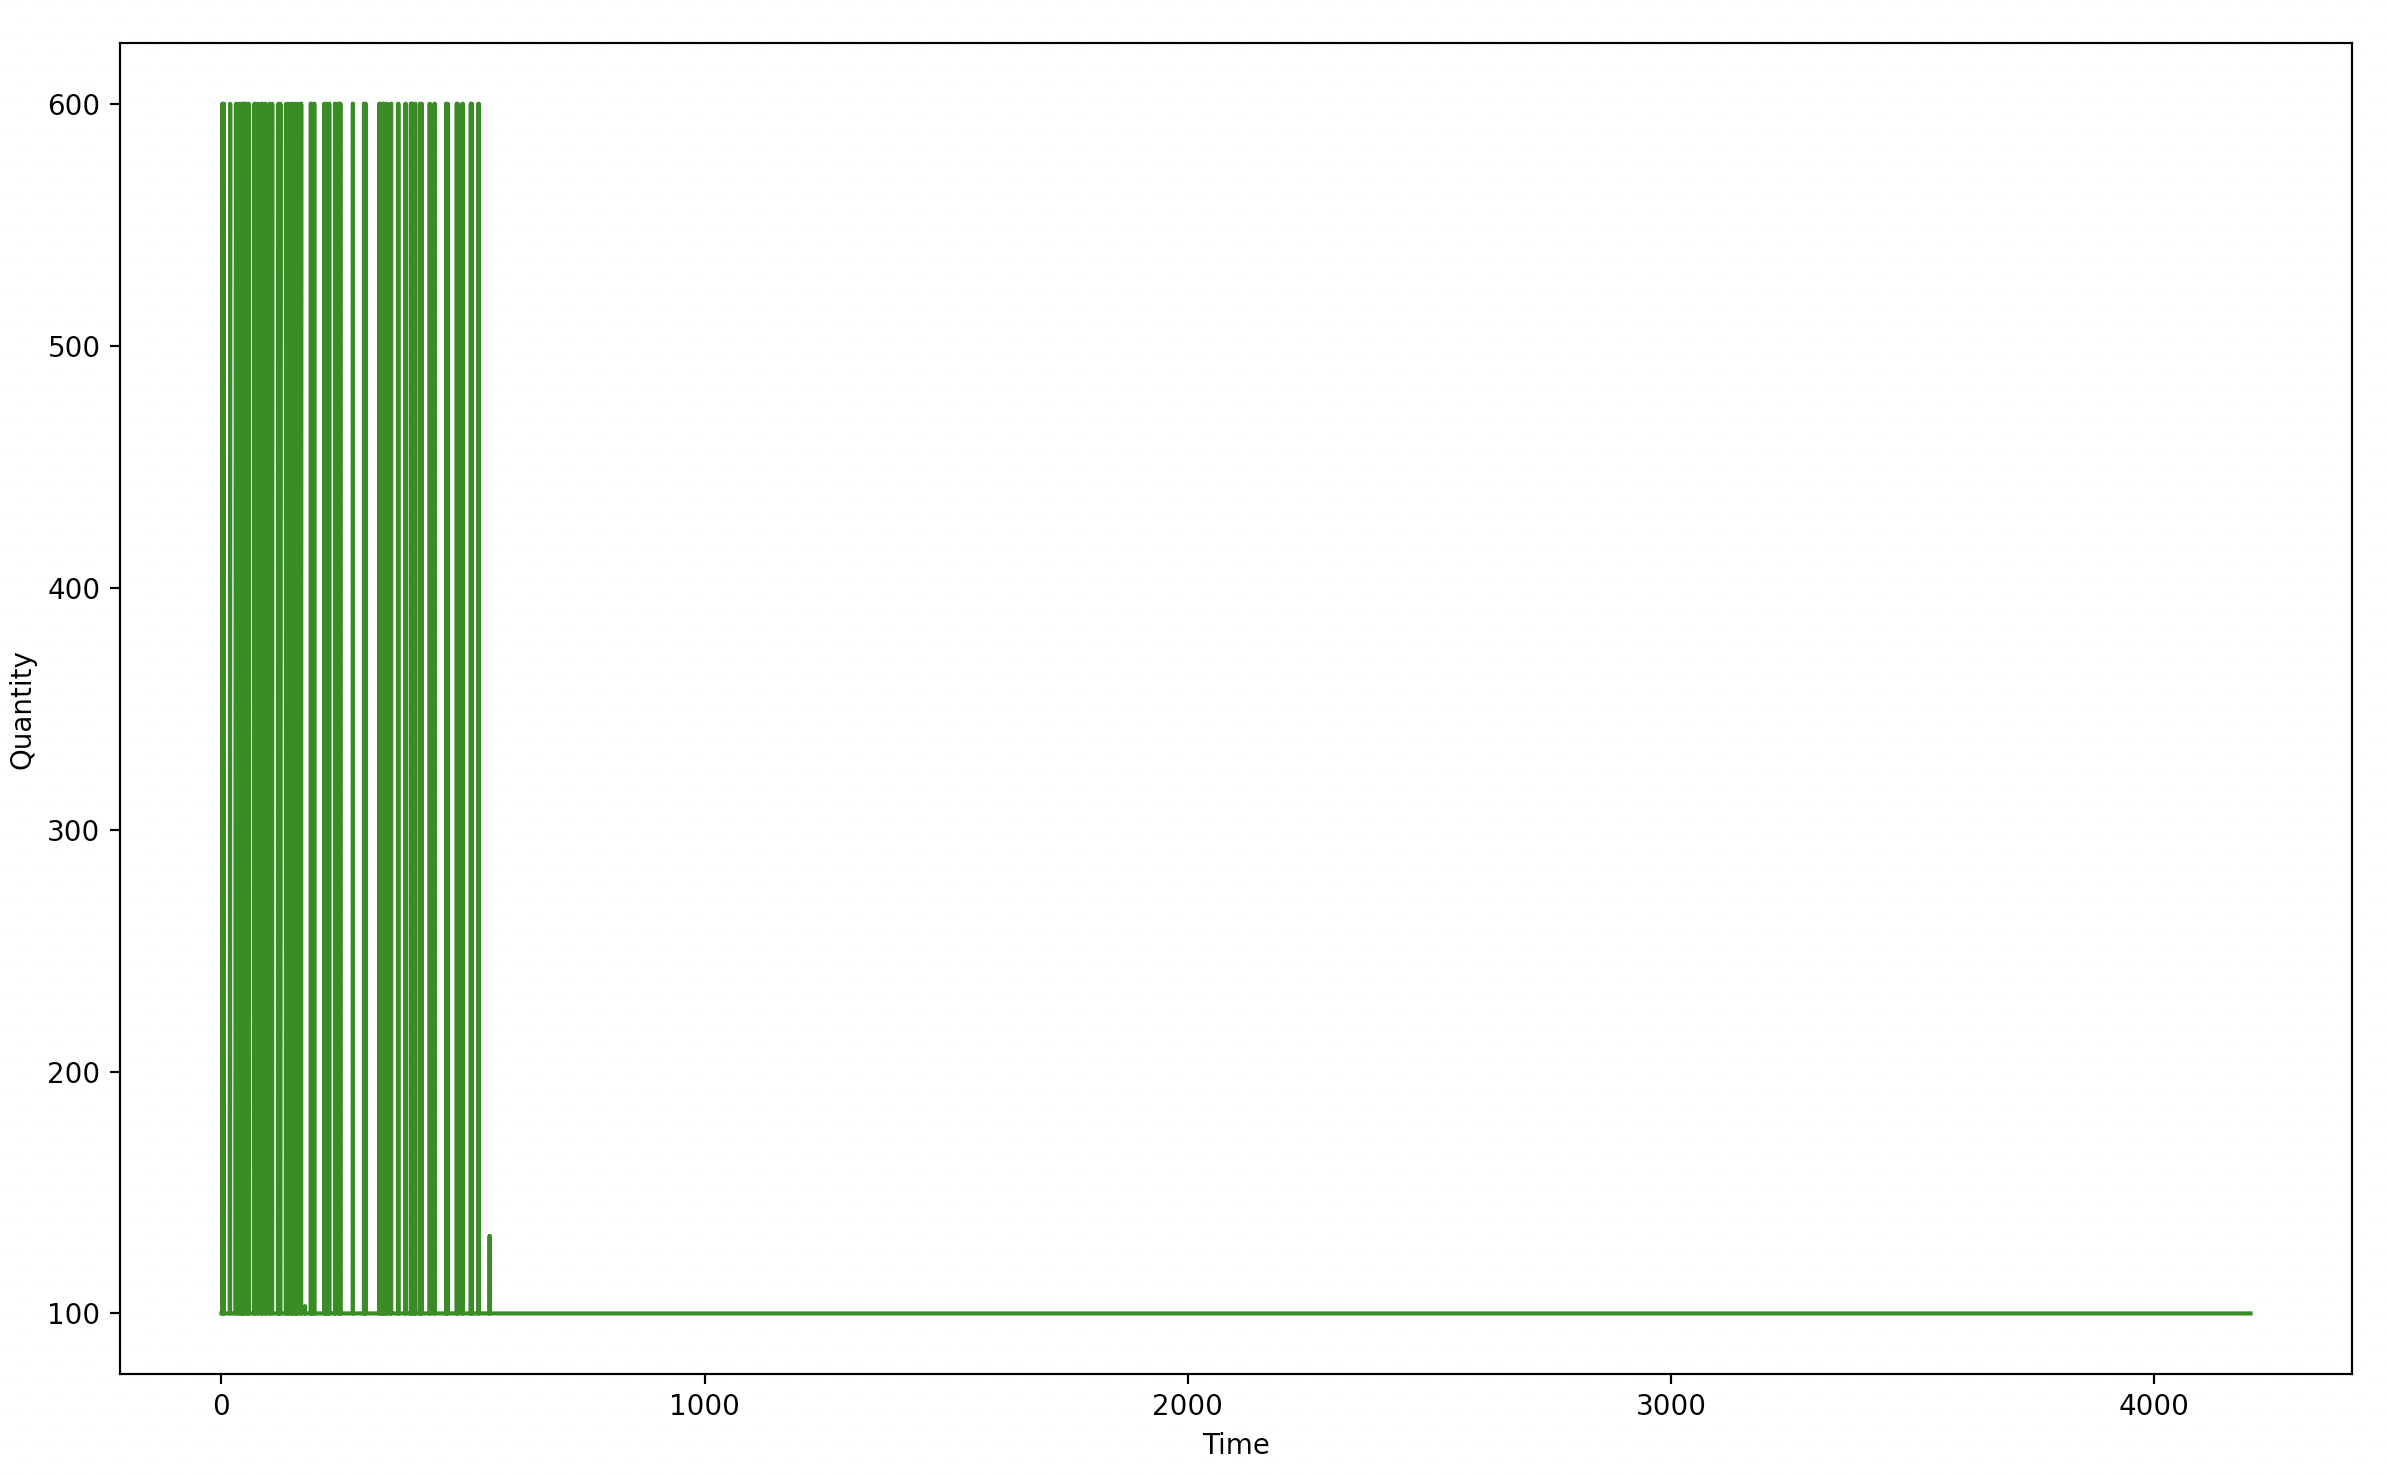
\includegraphics[width=7cm, height=6cm]{Dissertation/images/mcg_indv/LIQ/100.png}
    \caption{Case A : Simple seller quantity of 100 in 4200 McG action steps}
    \label{fig:liq_indv_1}
  \end{subfigure}
  %
  \begin{subfigure}[b]{0.5\textwidth}
    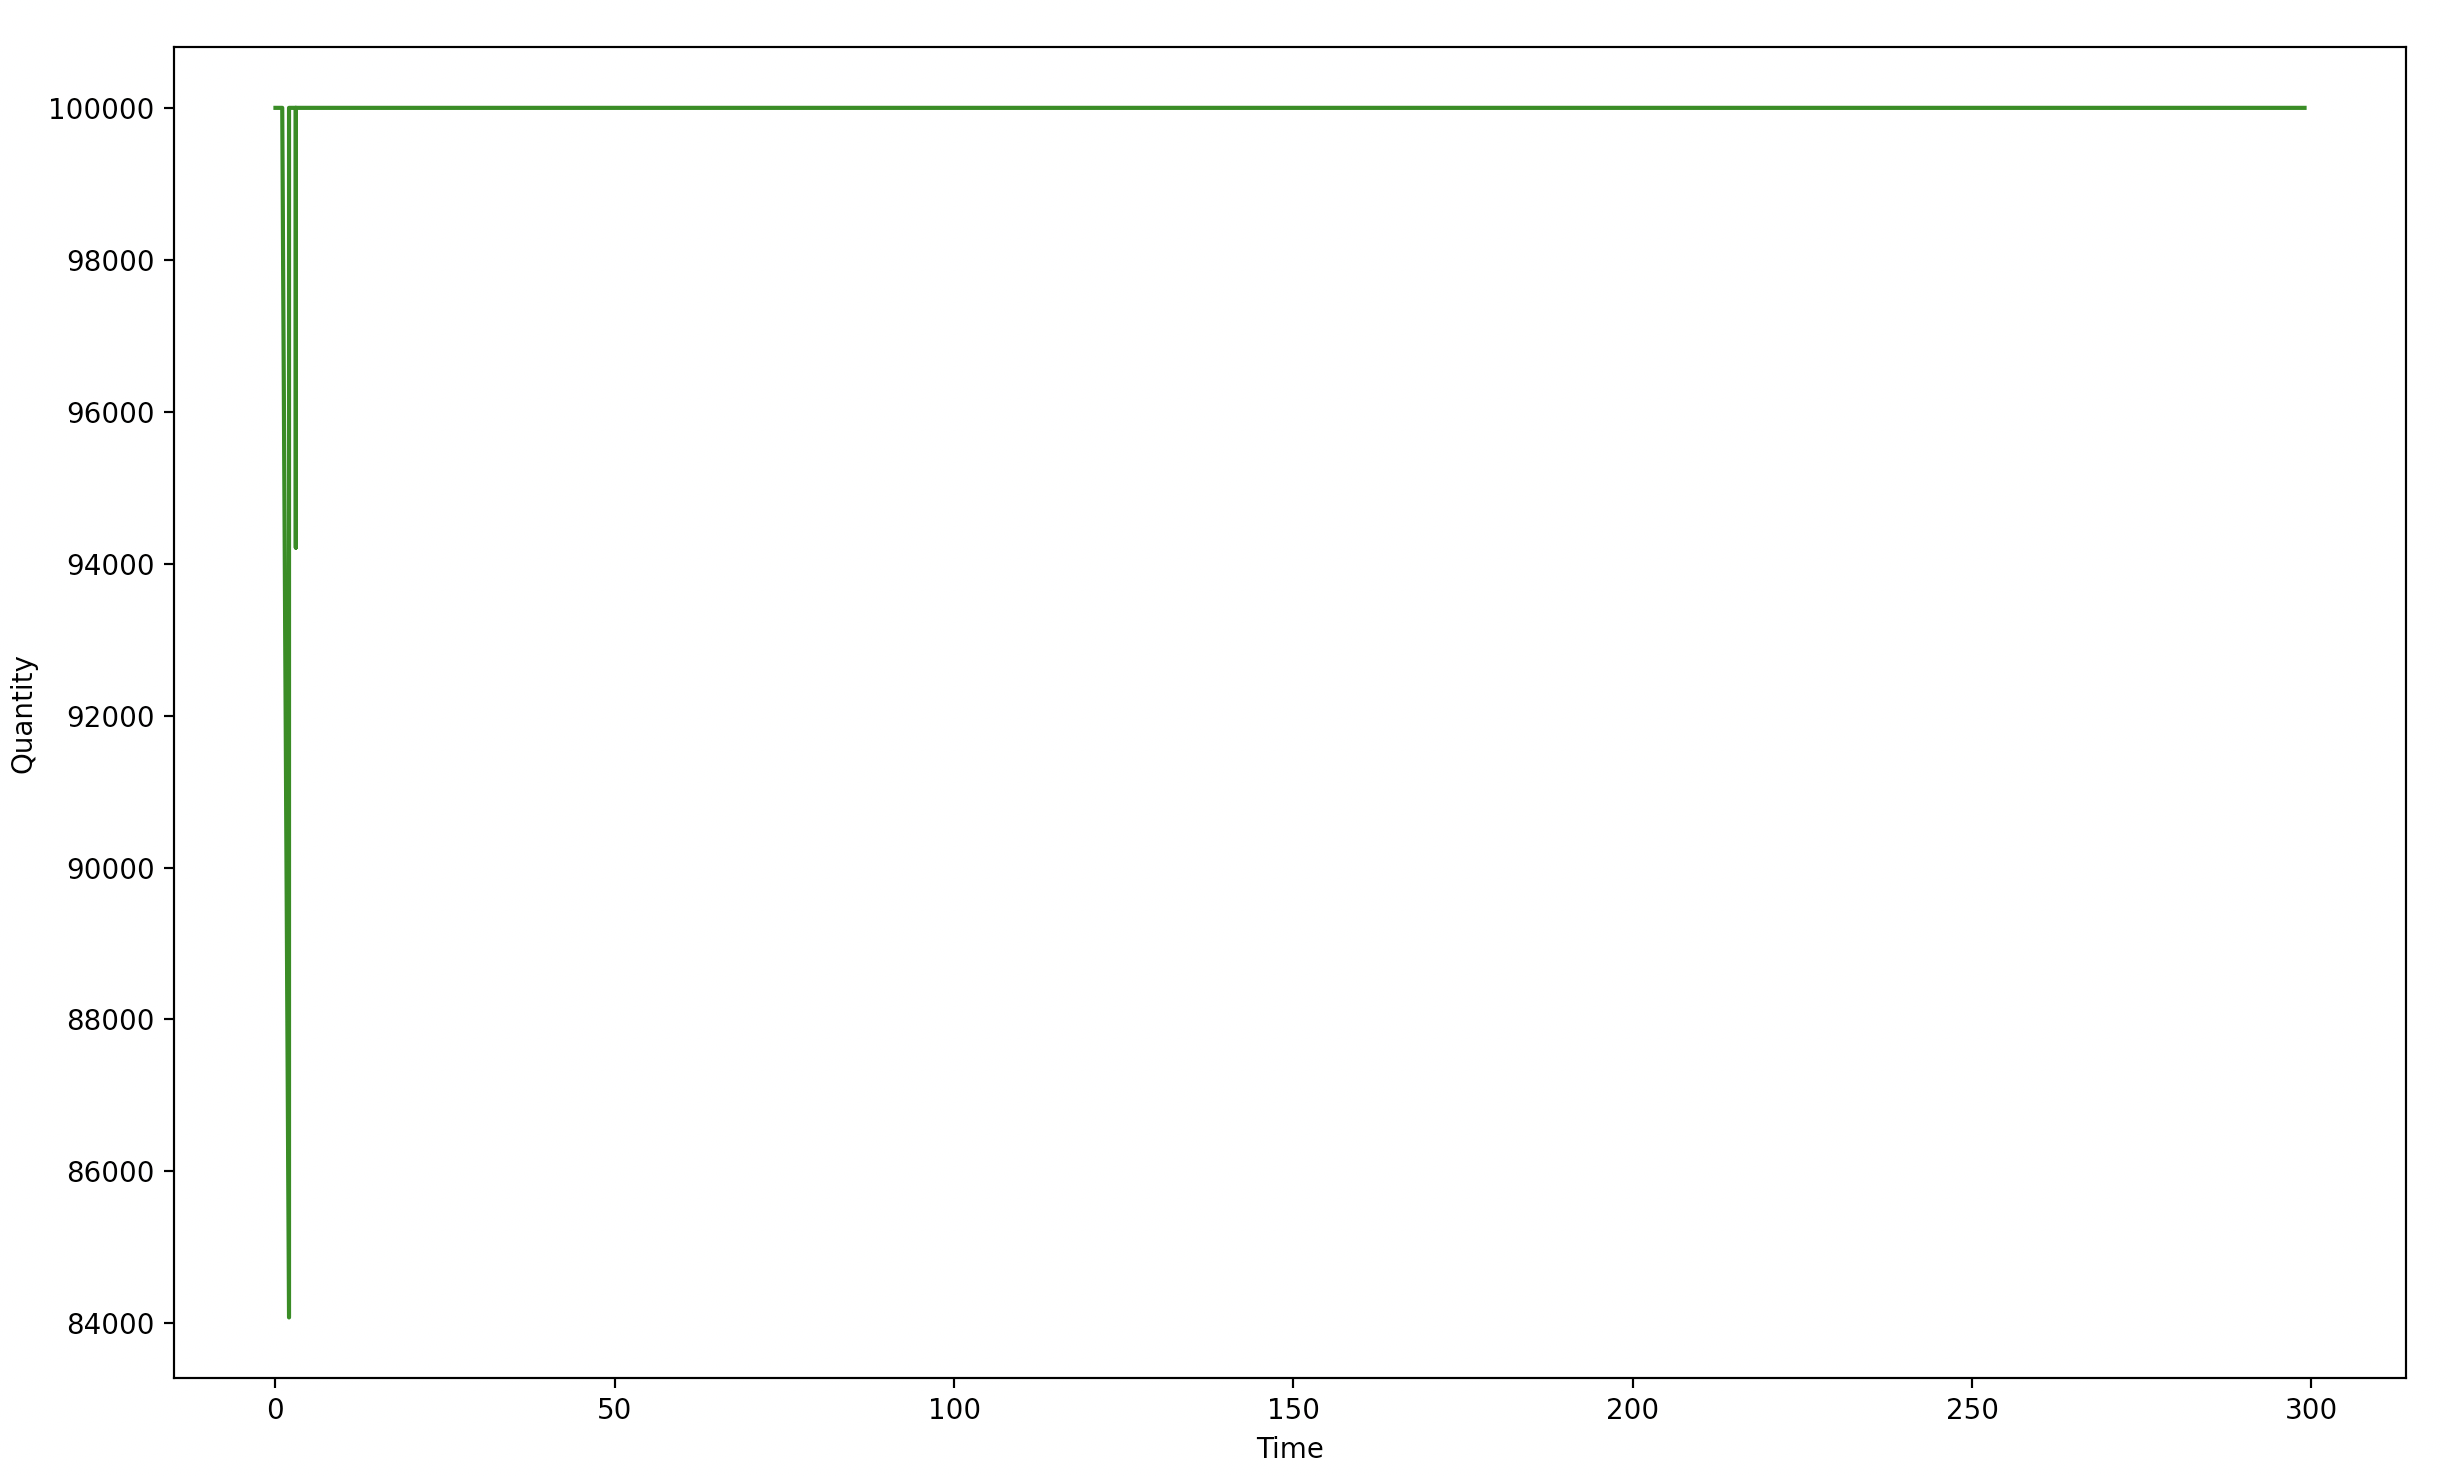
\includegraphics[width= 7cm, height=6cm]{Dissertation/images/mcg_indv/LIQ/san.png}
    \caption{Case B : Simple seller quantity of 100,000 in 300 McG action steps}
    \label{fig:liq_indv_2}
  \end{subfigure}
\caption{Quantity of each order submitted : Liquidity consumer with Simple Seller submitting different quantity of orders in 4200 McG action steps} 
\end{figure}
\FloatBarrier

\textbf{Case A:} The first case in Figure \ref{fig:liq_indv_1} is when the Simple sellers are only submitting orders at $price = 100$ and $quantity = 100$. It can be seen that in the initial period of the market, the orders submitted is 600. Theses are all orders submitted by the Liquidity consumer agents because their initially drawn large order is much higher than what is available in the market. The number is 600 because there are 6 Simple sellers who are all submitting orders of 100 quantity. Hence, they submit what is the maximum quantity at the best price of the opposite side of the book which is directly in Condition 2 on Line 8 in Algorithm \ref{algo:liquidity_consumer}. 

\textbf{Case B:} The second case in Figure \ref{fig:liq_indv_2} is when Simple sellers are submitting at $price = 100$ and $quantity = 100,000$. This means that traders who have been assigned with "Bid" day task will submit their initial large order and then stop after submitting one order because they are able to submit their whole large order since the orders at the opposite side of the book is much larger than their initial large order. This is because the agents' large is drawn uniformly from 1 to 100,000 while the Simple agents are submitting at only 100,000. The smaller values than 100,000 in the initial period of the market is from Liquidity consumer submitting their whole initially drawn large orders. This is Condition 1 on line 10 of the Algorithm \ref{algo:liquidity_consumer}. The rest of the orders seen in the market at 100,000 quantity is from only Simple Sellers.

The case where there are only Simple Buyers is omitted because the results would be similar except the Liquidity consumer would only submit ask orders because there are only bid orders in the LOB. 


\section{Momentum trader}
The momentum trader is one of two the high frequency trader who submit according to the market current price movement. A momentum trader trades depending on the rate of change in the price movement. The trader will submit a bid order if the price has recently been rising and an ask order otherwise. The calculation of Rate of Change (ROC) is given by: 
\begin{equation}
    roc_t = \frac{p_t - p_{t-n_r}}{p_{t-n_r}}
\end{equation}
\newline where $p_t$ = price at time t, $n_r$ = the period where the agent will calculate the ROC 

\newline When $roc_t$ is greater than some threshold $\kappa$, the agent submits a bid order with the volume described as:
\begin{equation}
     v_t = \abs{roc_t} * W_{a,t} 
\end{equation}
\newline where $roc_t$ = ROC at time t, $W_{a,t}$ = the wealth of the agent at time $t$. 

\begin{algorithm}[H]
\DontPrintSemicolon 
\If{$random() < \delta_{mt}$} {
    \tcc{Condition 1} 
    \If{$roc_t \ge \kappa$} {
    Submit market buy order with volume $v_t = \abs{roc_t} * W_{a,t}$\;
    }
    \tcc{Condition 2} 
    \uElseIf{$roc_t \leq -\kappa$}{
    Submit market sell order with volume $v_t = \abs{roc_t} * W_{a,t}$;\
    }
    \EndIf
  }
\EndIf
Update ROC $roc_t = \frac{p_t - p_{t-n_r}}{p_{t-n_r}}$\;  
\caption{{\sc Momentum trader reproduced from McG (4.3) \cite{McGroarty} } }
\label{algo:momentum}
\end{algorithm}

\begin{table}[h]
\centering
\begin{tabular}{ |m||p{4cm}|} 
\hline
\textbf{Momentum trader Parameters}& \textbf{Value} \\
\hline
\hline
$n_r$ & 5 \\ 
\hline
$\kappa$ & 0.001\\ 
\hline
$V_{mt}$ & 500,000 (100,000 in the test) \\ 
\hline
\end{tabular}
\caption{Momentum trader parameters taken from \cite{McGroarty}} 
\end{table}
\FloatBarrier 

\subsection{Momentum trader's Wealth}
One of the important variable in the Momentum trader's trading strategy is its wealth. The agent will submit the quantity of an order based on its wealth given by equation : $v_t = \abs{roc_t} * W_{a,t}$. The concept of Wealth $W_{a,t}$ is different in this BSE implementation due to the fact that the agent can submit either a bid or an ask in any order. In reality, a trader can submit an ask then buy back the stocks at a later date. Similarly, one can buy a quantity of stock and sell it back at a later date. Because the Momentum trader does not have that constraint, there must be some abstraction in calculation of wealth. 

The approach taken in this project is as follow: The wealth will be separated into two types : Ask balance and Bid balance. 

\begin{itemize}
  \item \textbf{Ask Balance} : The initial price is 0. This is due to the fact that if someone sells a product, their wealth will increase. After the agent's market order is fulfilled, their ask balance will increase by $quantity * price_{transaction}$. This idea is abstracted from the fact that the agent can sell something it does not have. The ask balance will be capped at $V_{mt}$. 
  \item \textbf{Bid Balance} : The initial price is $V_{mt}$. This is due to the fact that if someone buys a product, their wealth will decrease. After the agent's market order is fulfilled, their bid balance will decrease by $quantity * price_{transaction}$.
\end{itemize}

The wealth $W_{a,t}$ of the agent is then calculated by Ask balance + Bid balance. 

\subsection{Momentum trader Test} 
Similar to Liquidity consumer, the Momentum trader submits only a market order. Hence, in the following experiment, only the quantity and the type of order will be investigated.  

The experiment will consists of two types of price arrangement : increasing and decreasing. This is to investigate whether the momentum trader will respond correctly to the momentum in the price. In order to evaluate the current Momentum trader algorithm, the following test will be conducted. The Simple Seller and Buyer will be modified such that:
\begin{itemize}
  \item It will include a probability of submitting at 0.25 to ensure that the orders don't always match and there is limit orders left in the Limit Order book. 
  \item The Simple agents will submit with quantity drawn uniformly from between 100 and 1000 to ensure that the Limit Order Book is not empty
  \item The agents will submit either a decreasing or increasing price in each iteration. For example, if it is decreasing, the initial price will be 1000 and decremented by 1 in each McG action step. This ensures that the mid price will be a downward slope and the momentum of the market is in the downward slide. 
\end{itemize}

The experiment will run in 1000 McG action step. The market consists of 6 Simple Buyers, 6 Simple Sellers and 6 Momentum trader. The results are illustrated below: 

\begin{figure}[h]
  \begin{subfigure}[b]{0.5\textwidth}
    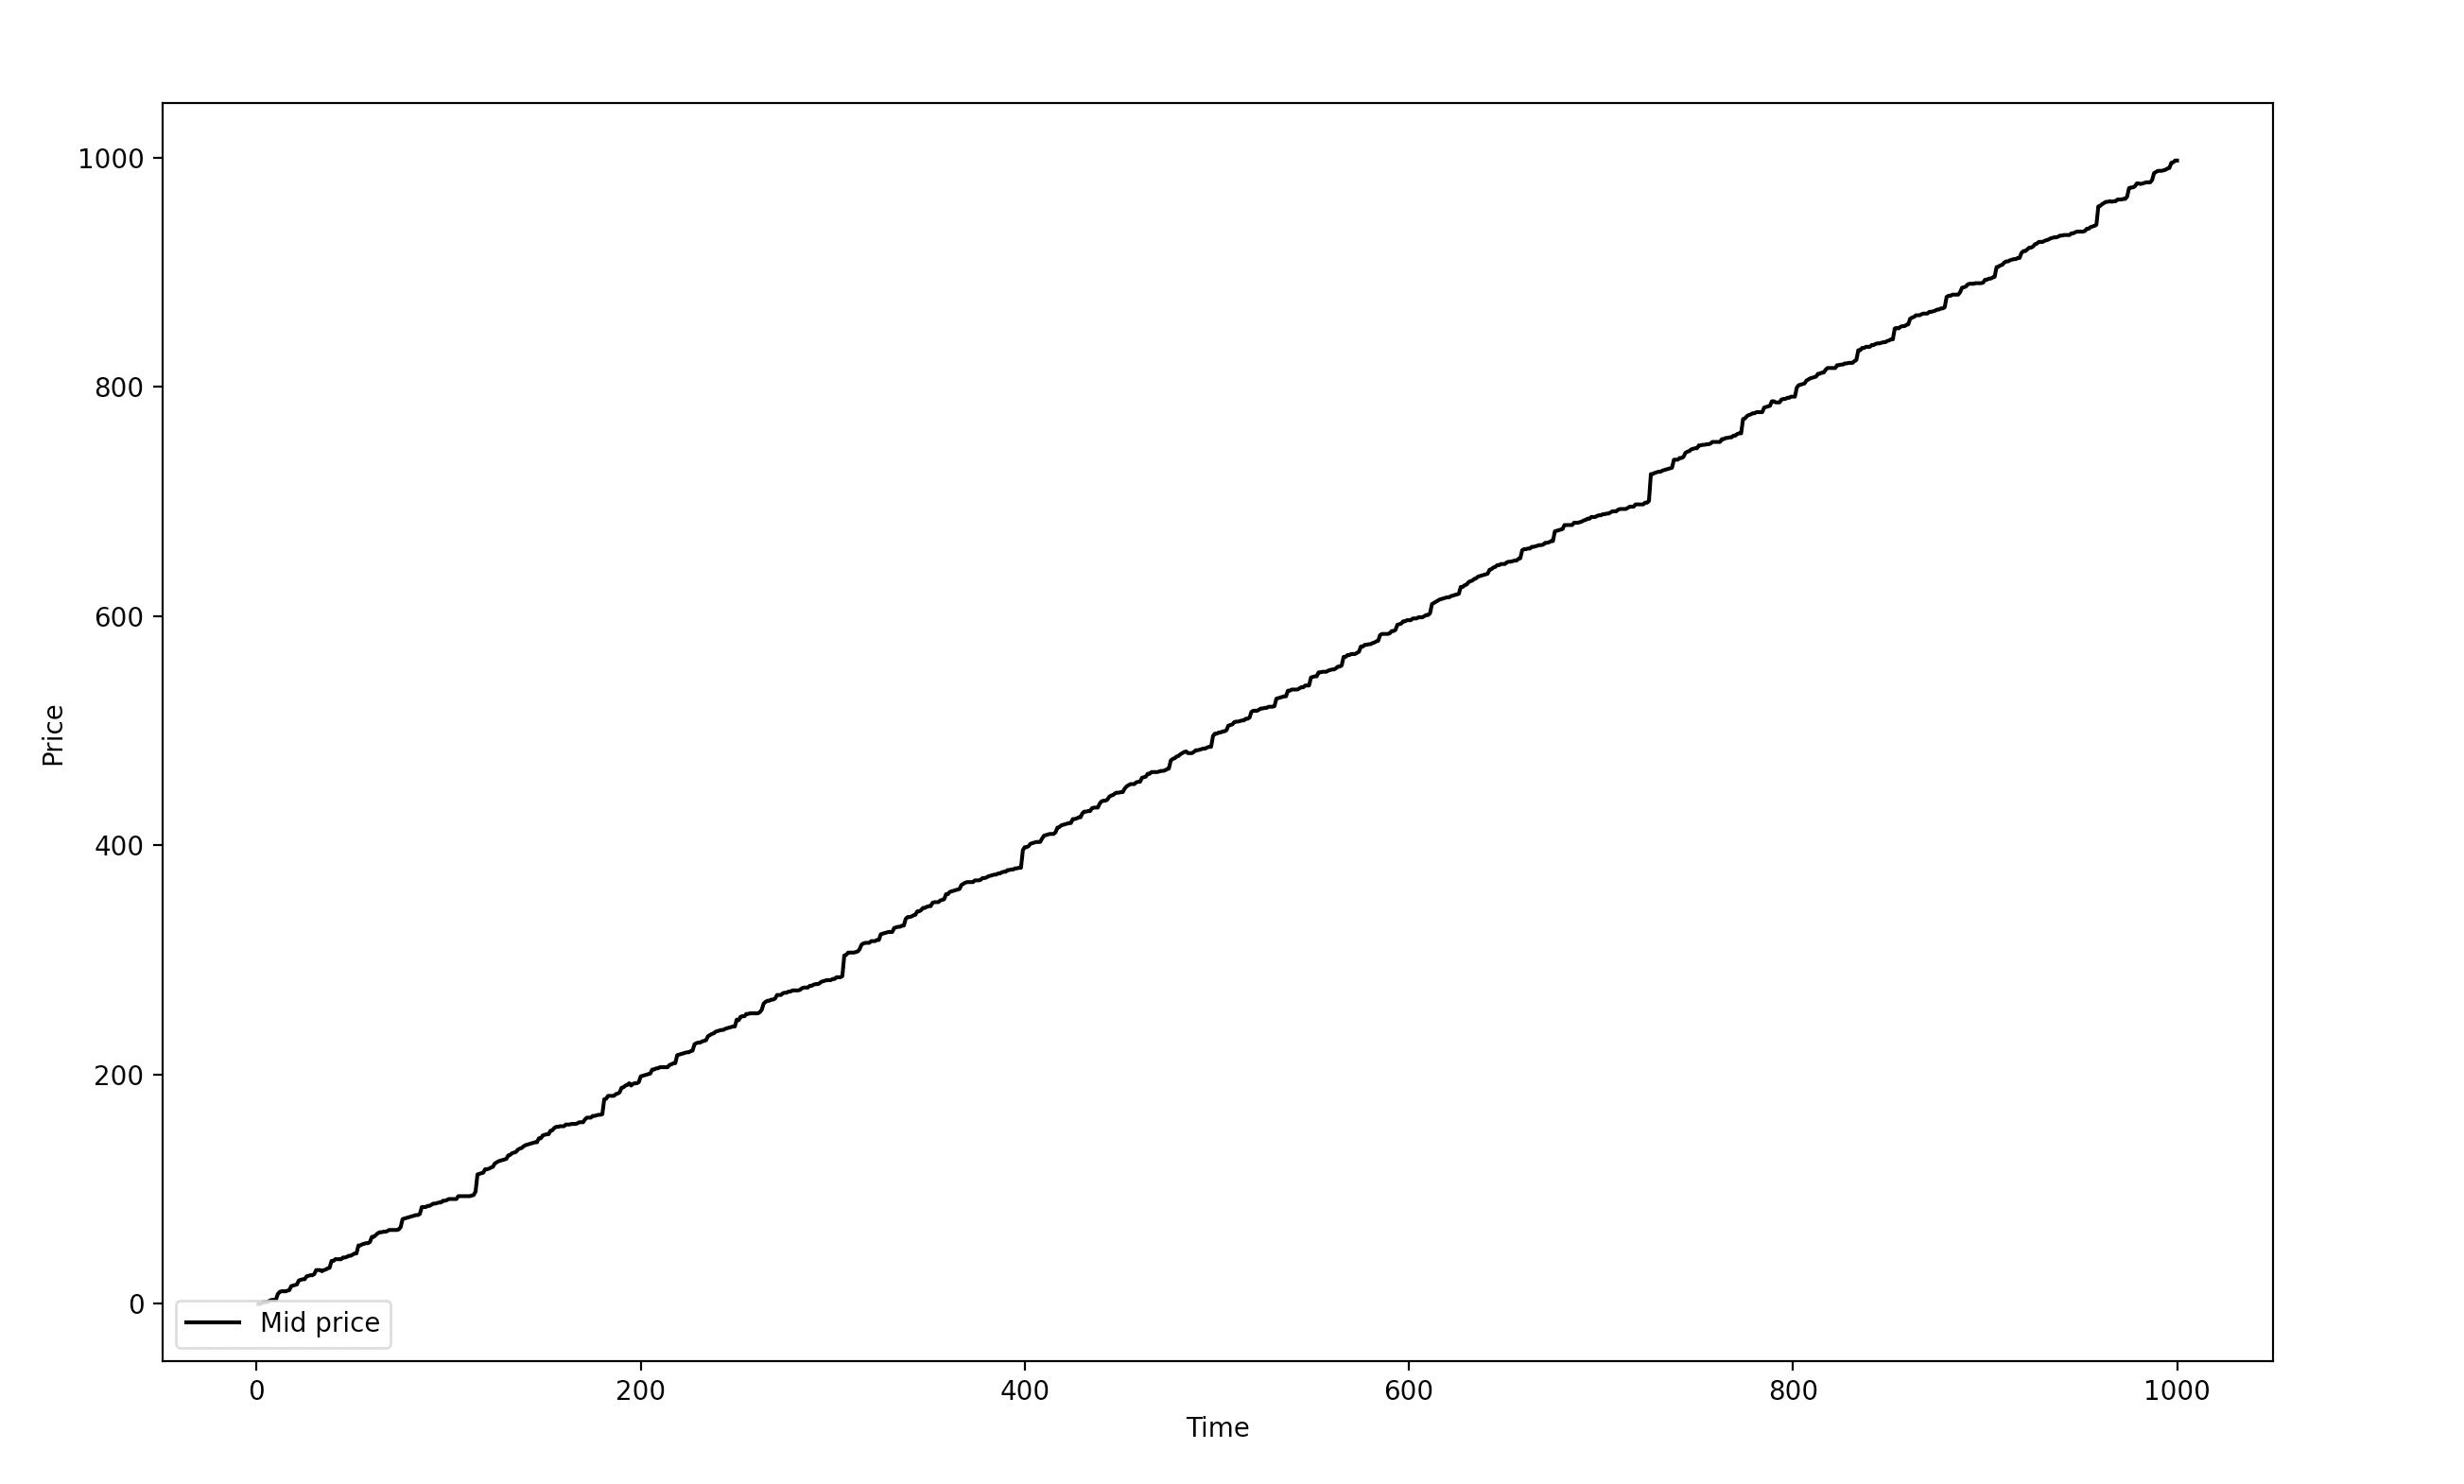
\includegraphics[width=7cm, height=6cm]{Dissertation/images/mcg_indv/MMT/incr.png}
    \caption{Mid Price}
    \label{fig:mmt_inc_midprice}
  \end{subfigure}
  %
  \begin{subfigure}[b]{0.5\textwidth}
    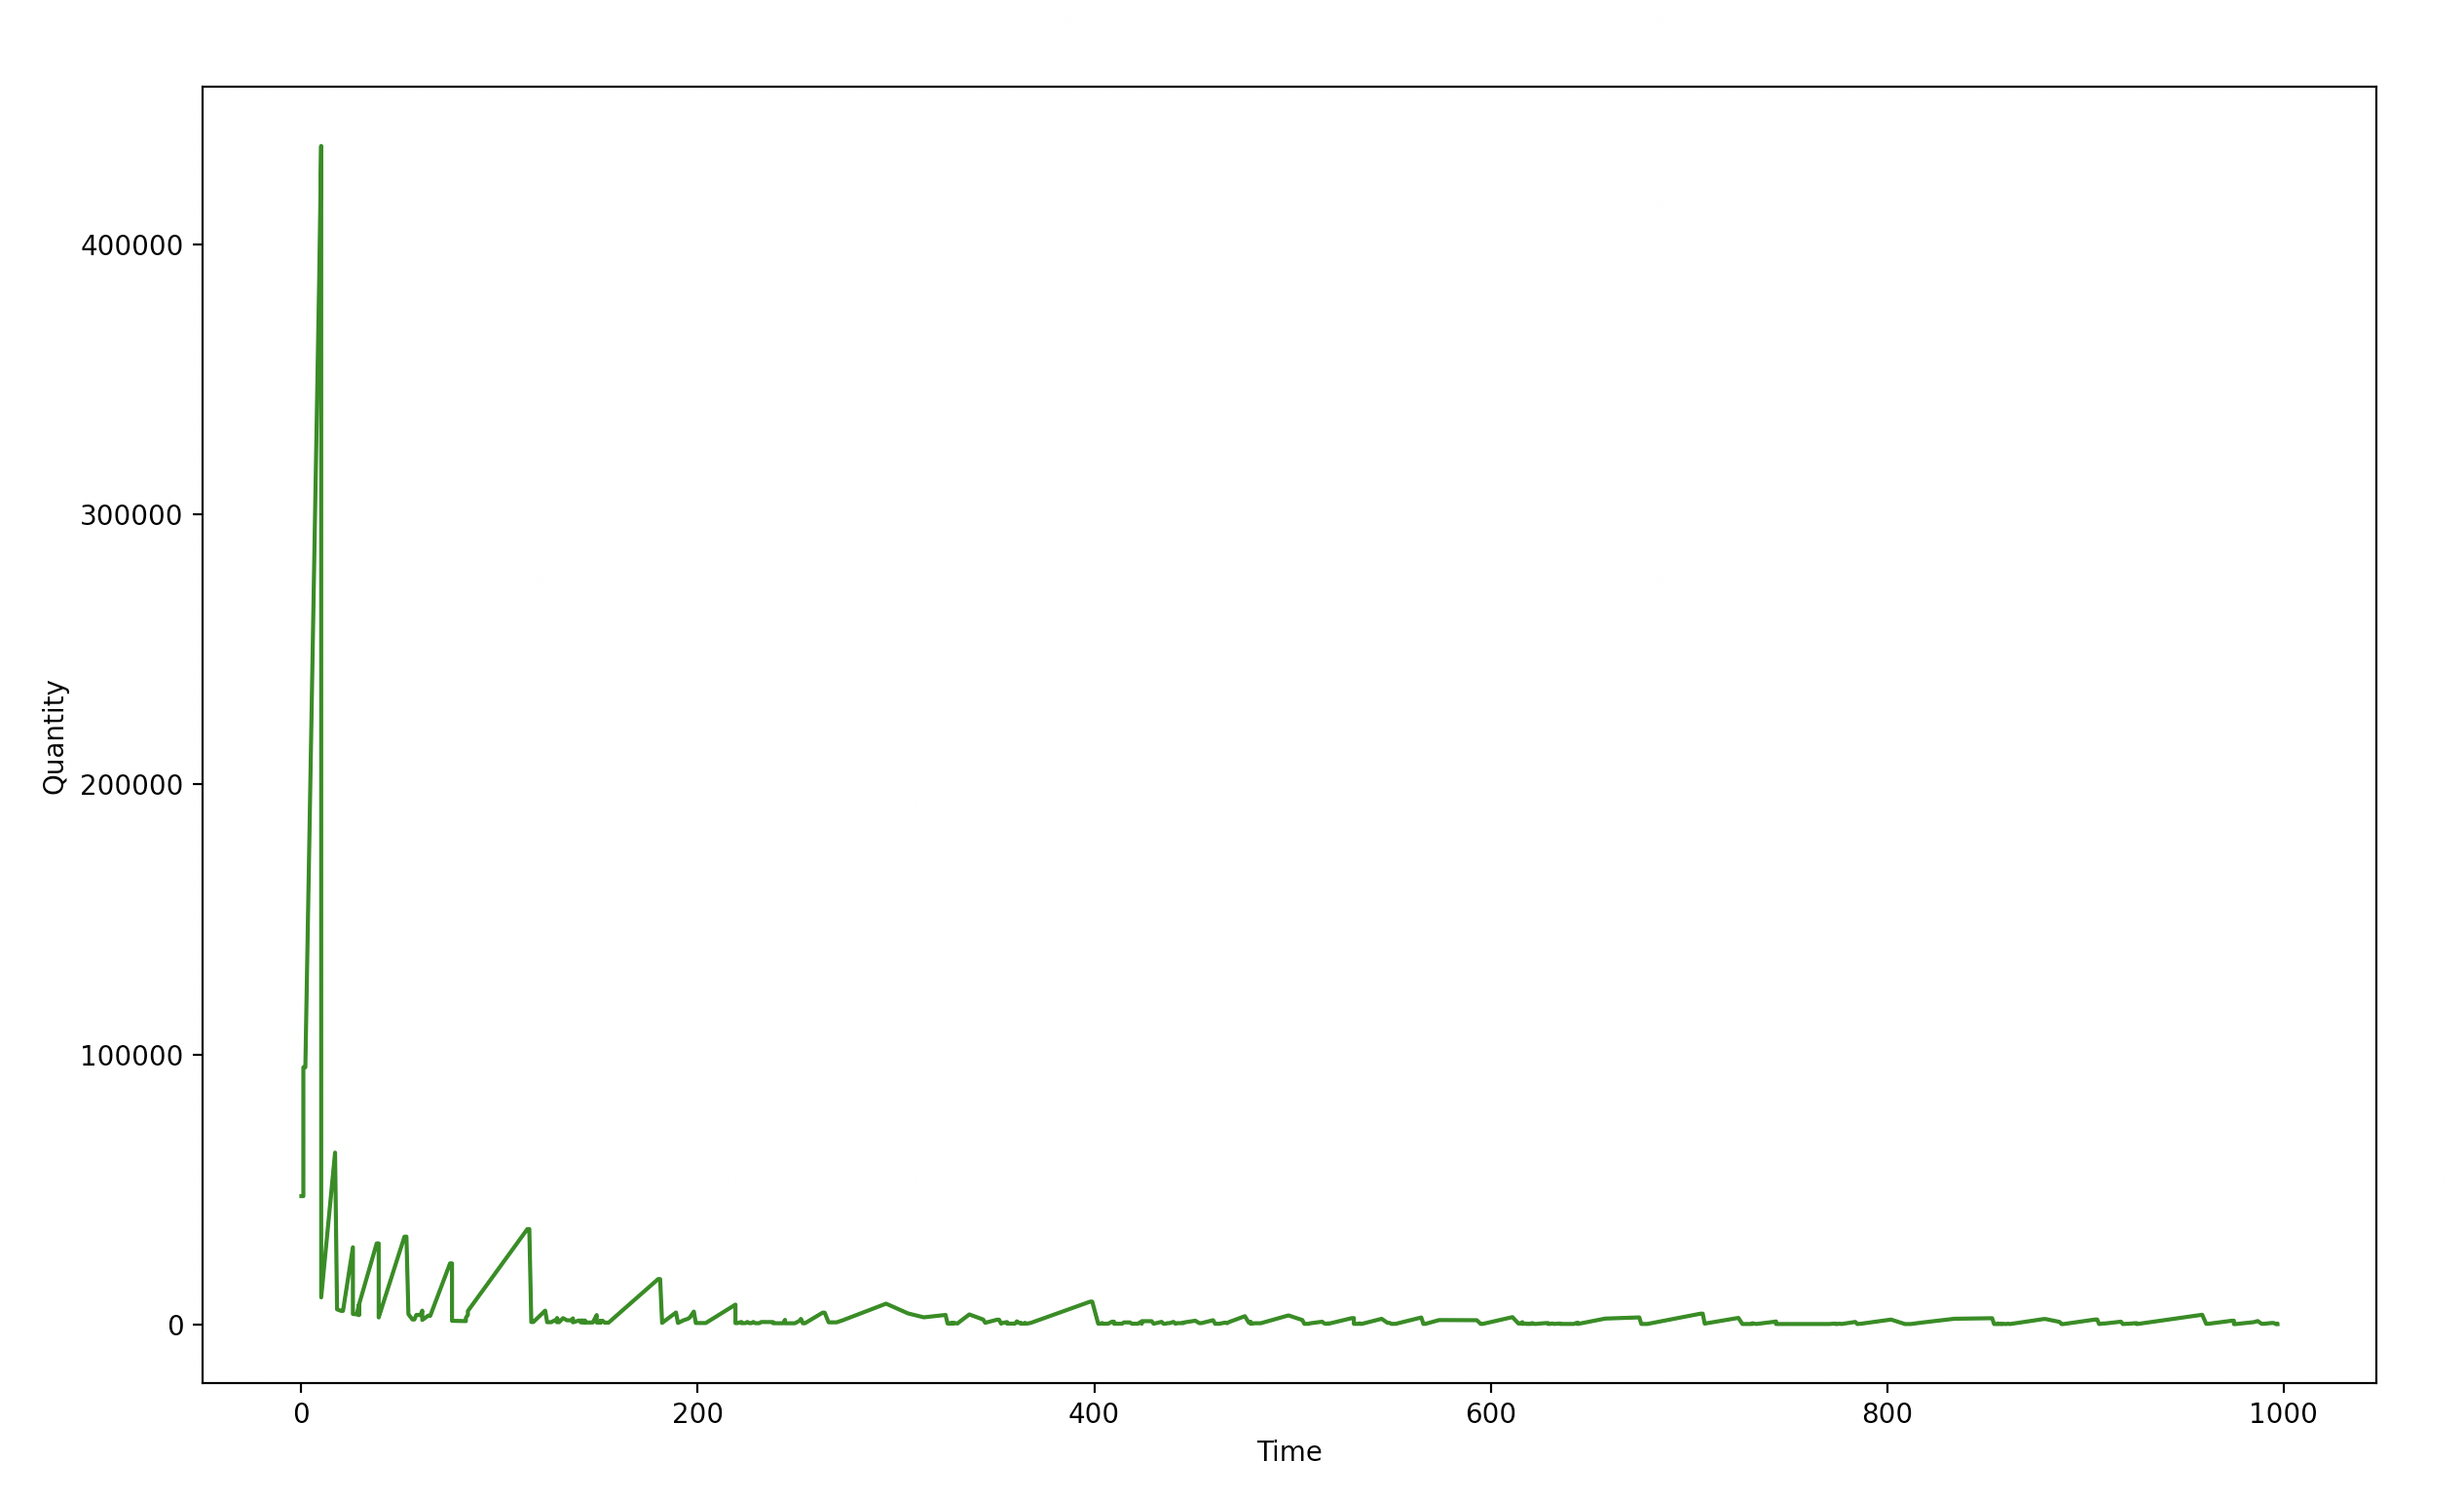
\includegraphics[width= 7cm, height=6cm]{Dissertation/images/mcg_indv/MMT/incr_qty.png}
    \caption{Quantity submitted by Momentum trader both Bid and Ask}
    \label{fig:mmt_inc_qty}
  \end{subfigure}
\caption{Momentum trader increasing price experiment} 
\end{figure}


\begin{figure}[h]
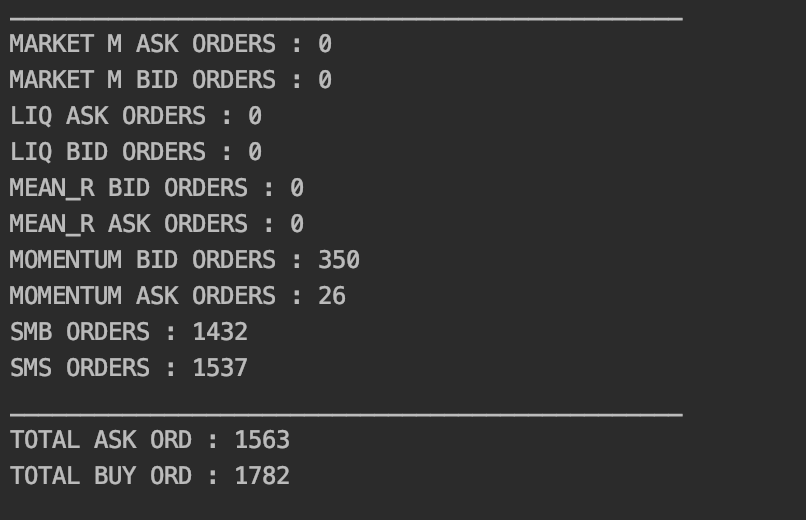
\includegraphics[ height=8cm]{Dissertation/images/mcg_indv/MMT/incr_stat.png}
\caption{Momentum trader increasing price experiment statistics} 
\label{fig:mmt_inc_stats}
\end{figure} 
\FloatBarrier

Figures \ref{fig:mmt_inc_stats}, \ref{fig:mmt_inc_qty} and \ref{fig:mmt_inc_midprice} illustrate the increasing test results of the market. Figure \ref{fig:mmt_inc_midprice} illustrates the mid price which increases over the 1000 time period. In Figure \ref{fig:mmt_inc_qty}, The quantity submitted by Momentum traders will quickly decrease because of the reduction in its wealth. This is because the agents are only buying because the momentum is going in upwards direction.This is directly from the line 2 or the first condition of the Algorithm \ref{algo:momentum}. 

In most cases, the price submitted from the trader at time t will be more than $t-n_r$. For example, if $p_t = 80$ then $p_{t - n_r} = 70$. This means that the $roc_t$ will be 0.114. According to the first condition of the Algorithm 4.3, $0.114 \ge 0.001$, which is true, the agent will submit a buy order, leading to the decreasing wealth described above.  

\begin{figure}[h]
  \begin{subfigure}[b]{0.5\textwidth}
    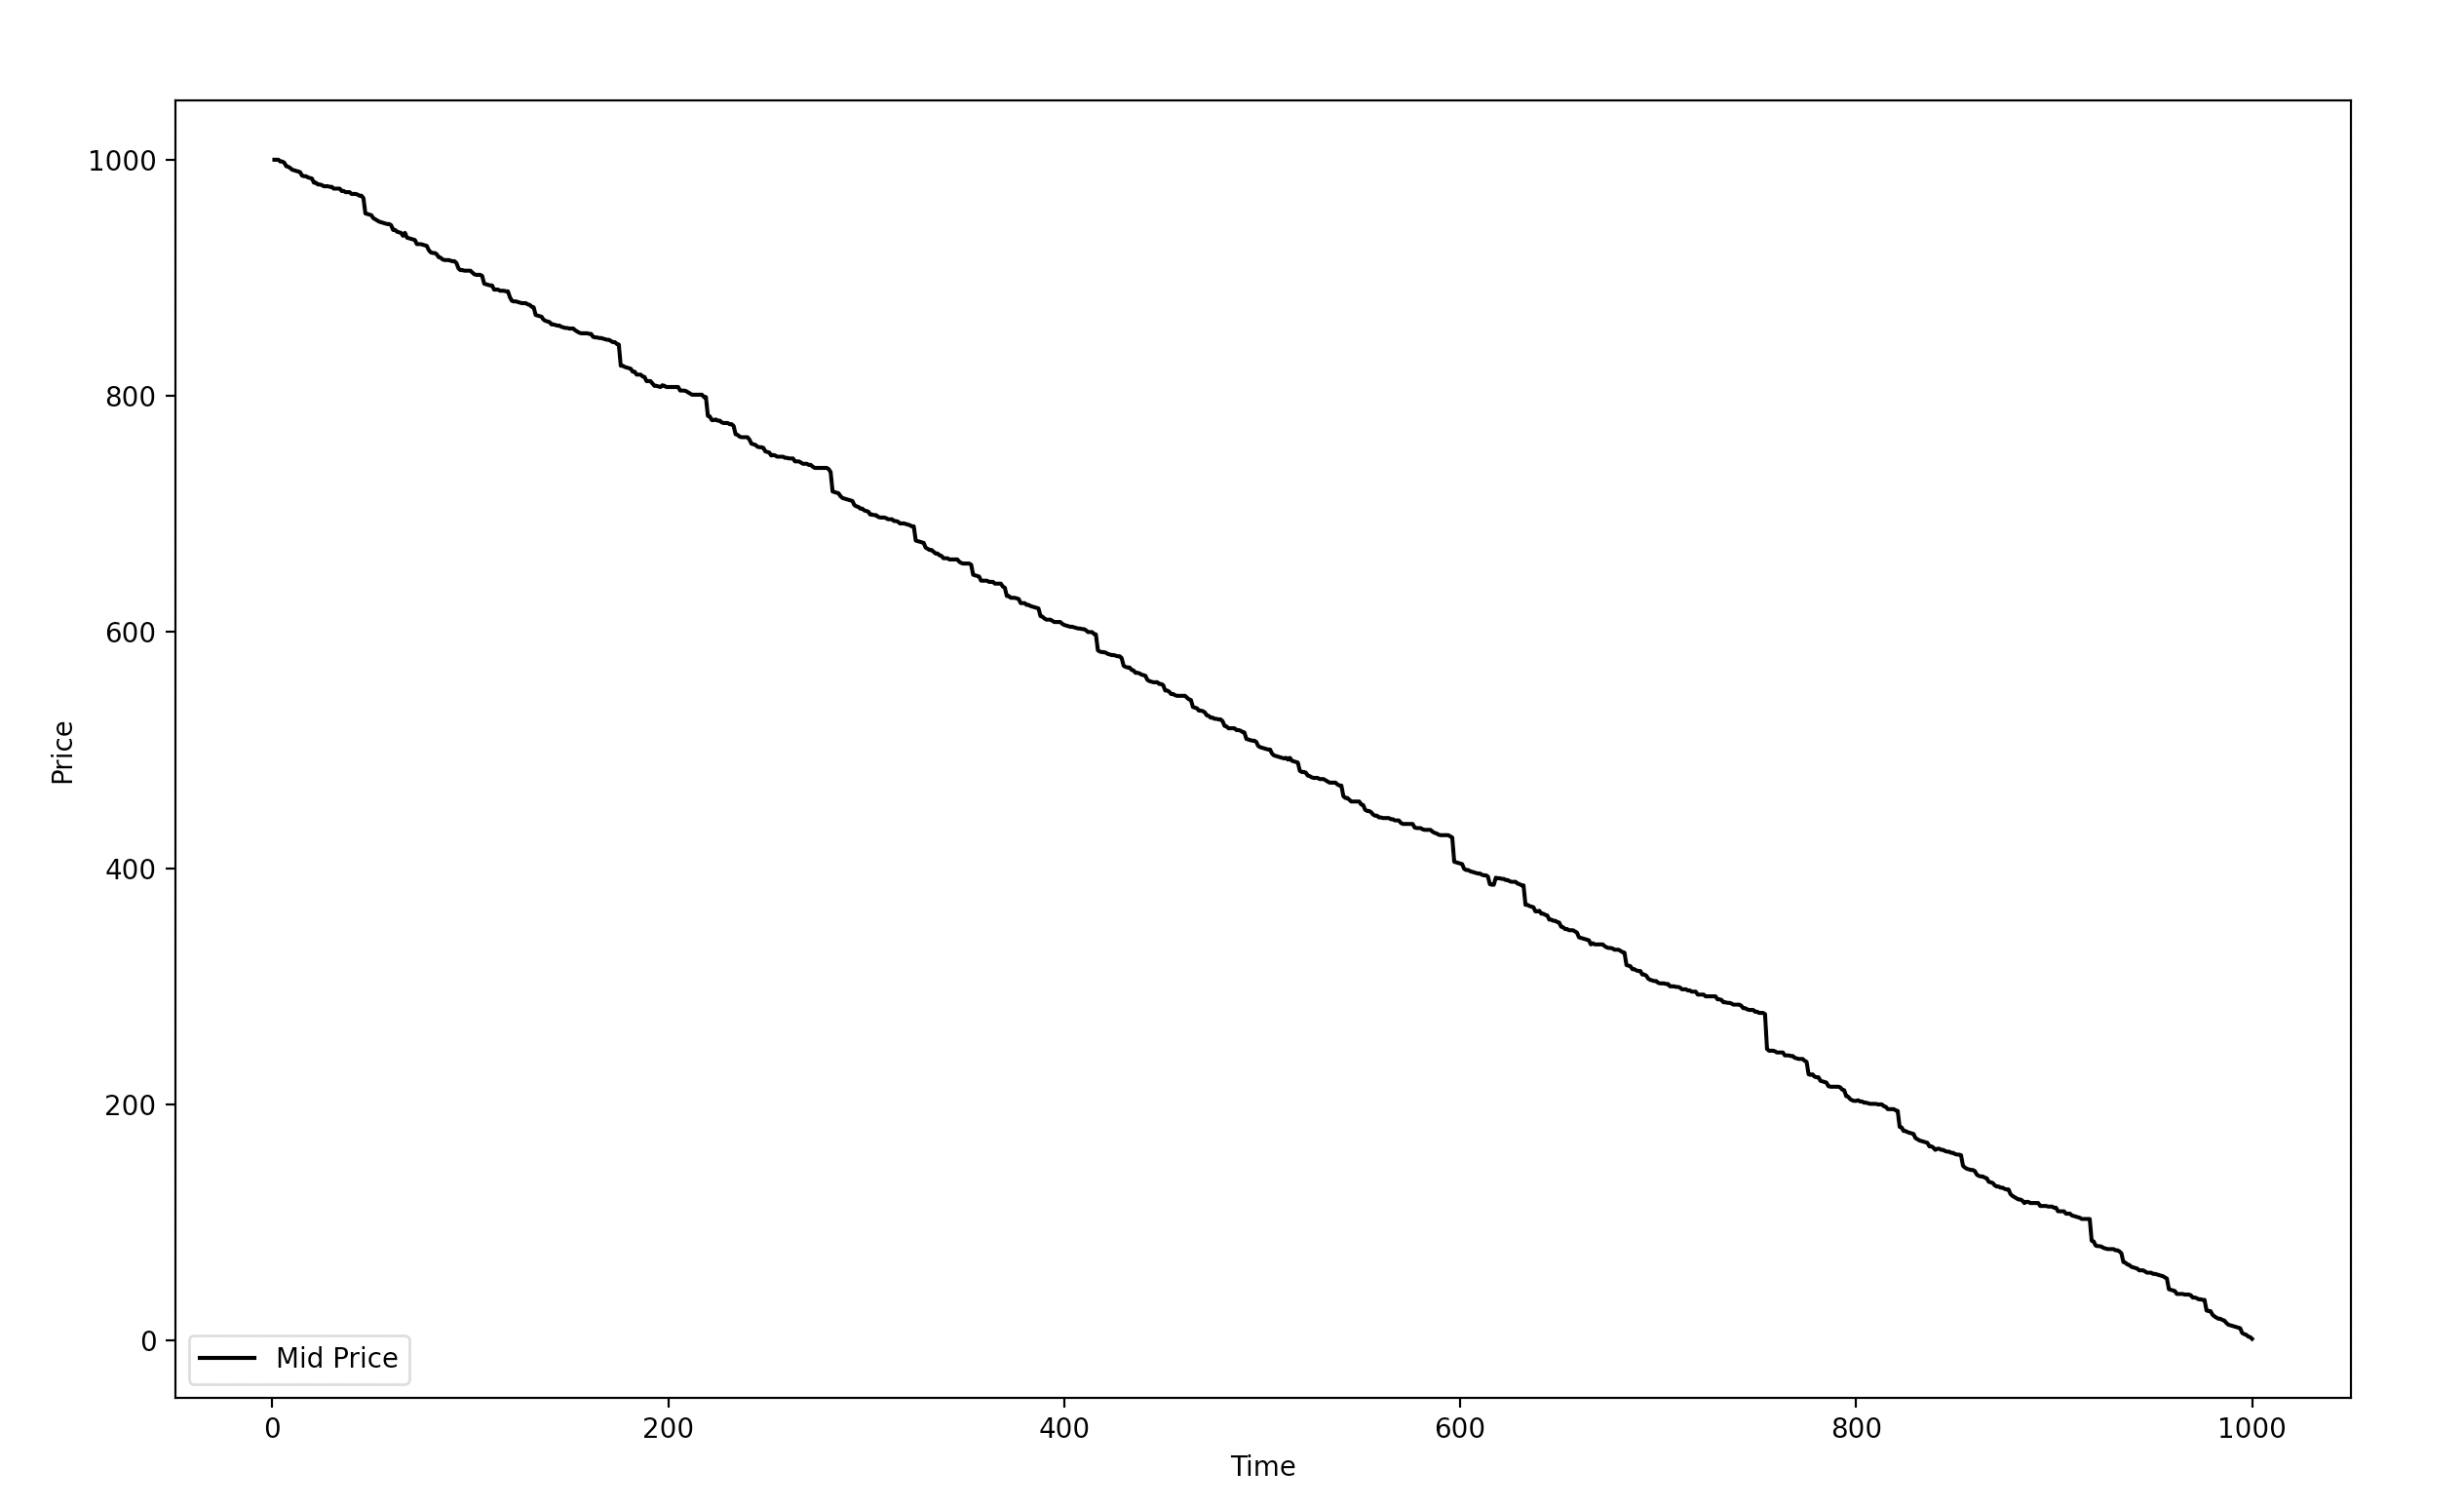
\includegraphics[width=7cm, height=6cm]{Dissertation/images/mcg_indv/MMT/dec_price.png}
    \caption{Mid Price}
    \label{fig:mmt_dec_midprice}
  \end{subfigure}
  %
  \begin{subfigure}[b]{0.5\textwidth}
    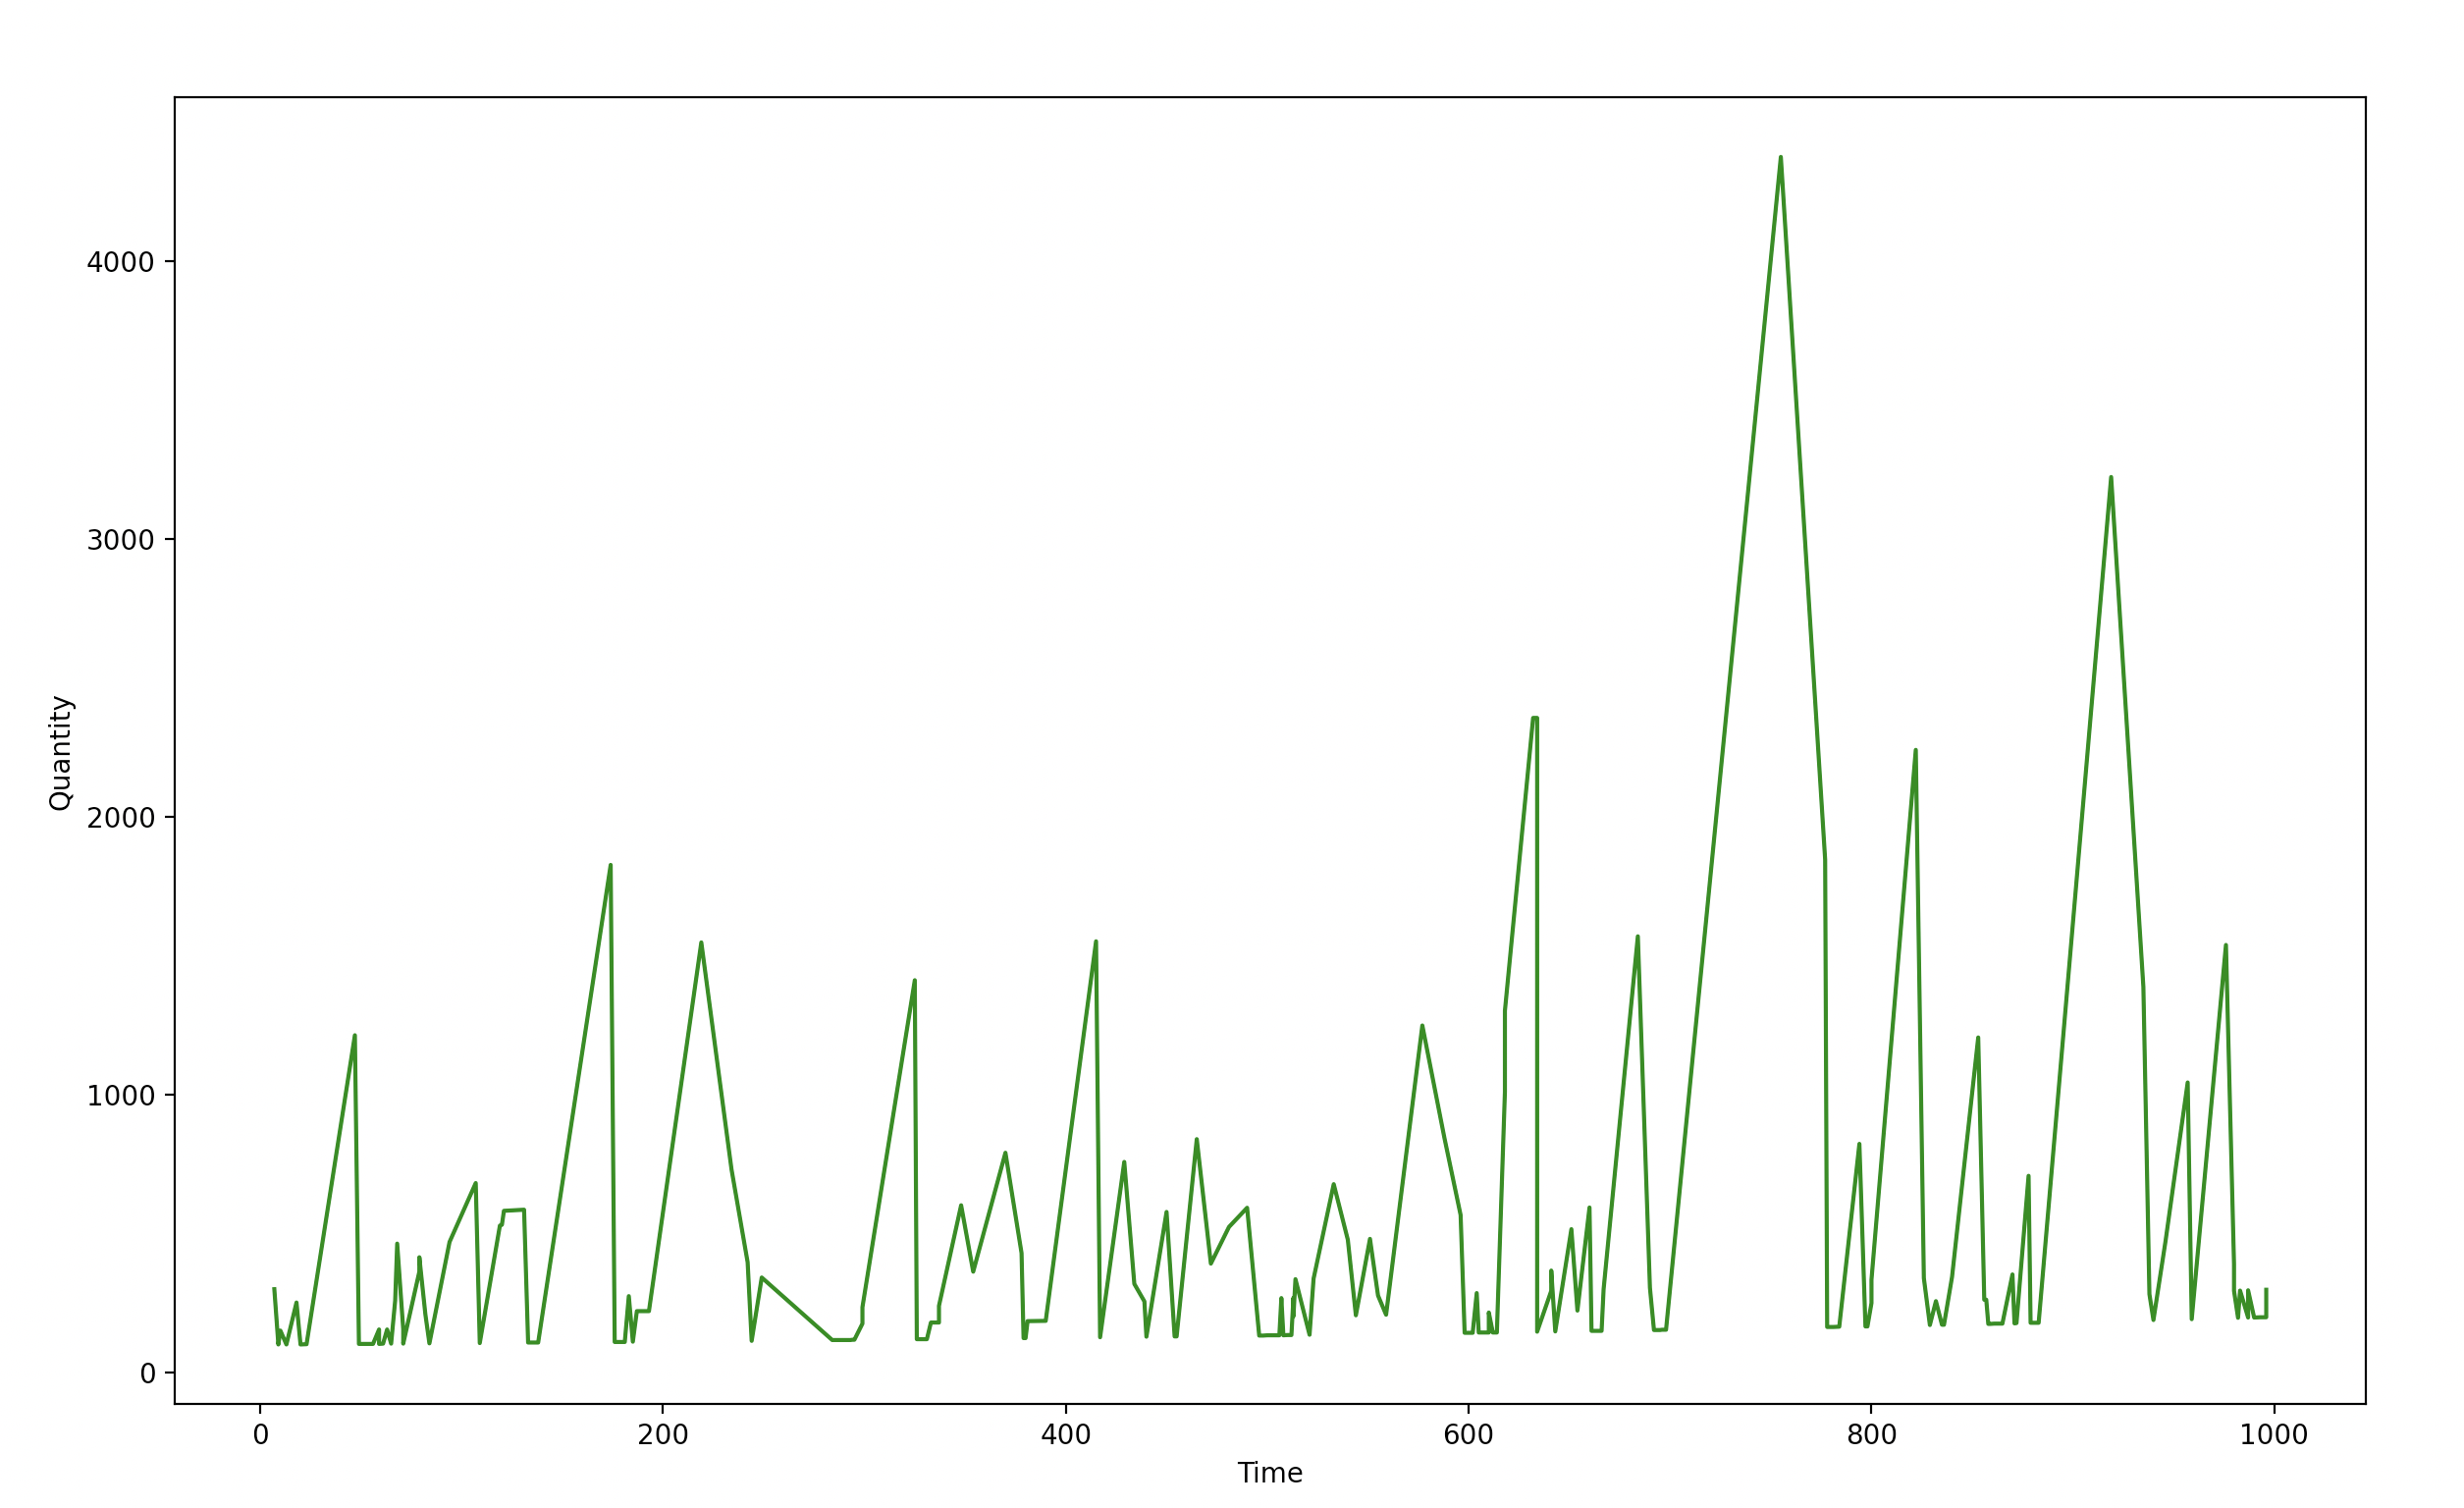
\includegraphics[width= 7cm, height=6cm]{Dissertation/images/mcg_indv/MMT/dec_qty.png}
    \caption{Quantity submitted by Momentum trader both Bid and Ask}
    \label{fig:mmt_dec_qty}
  \end{subfigure}
\caption{Momentum trader decreasing price experiment} 
\end{figure}


\begin{figure}[h]
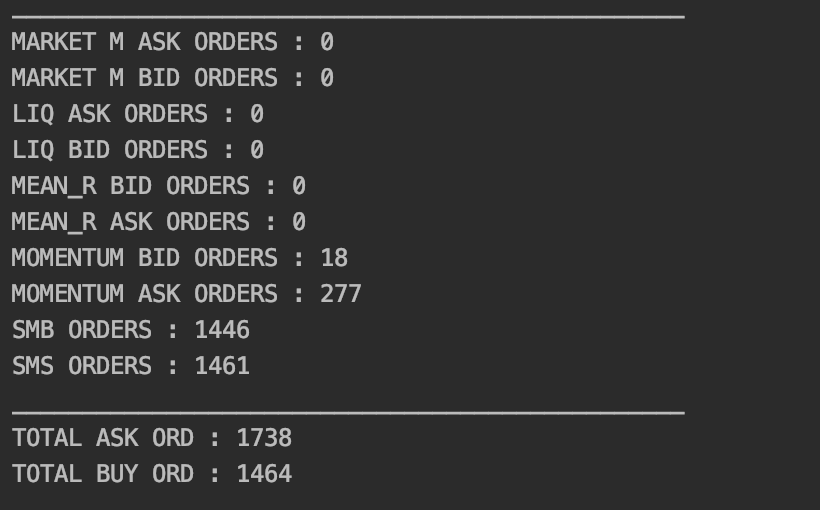
\includegraphics[ height=8cm]{Dissertation/images/mcg_indv/MMT/dec_stat.png}
\caption{Momentum trader decreasing price experiment statistics} 
\label{fig:mmt_dec_stats}
\end{figure} 
\FloatBarrier

Figures \ref{fig:mmt_dec_midprice}, \ref{fig:mmt_dec_qty}  and \ref{fig:mmt_dec_stats} illustrate the decreasing test results of the market. Figure \ref{fig:mmt_dec_midprice} illustrates the mid price which decreases over the 1000 time period. The quantity over time in this experiment is increasing since the agents are submitting only ask orders, hence their wealth is increasing over time. This is directly from line 4 or the second condition of the Algorithm \ref{algo:momentum} where we can see the Momentum of the market going downwards from Figure \ref{fig:mmt_dec_qty}. The majority of the order submitted in Figure \ref{fig:mmt_dec_stats} will be asks orders because the market is gaining an downward momentum. 

In most cases, the price submitted from the trader at time t will be less than $t-n_r$. For example, if $p_t = 70$ then $p_{t - n_r} = 80$. This means that the $roc_t$ will be $-0.125$. According to the second condition of Algorithm \ref{algo:momentum}, $-0.125 \leq -0.001$, which is true, the agent will submit a sell order, leading to the increasing wealth described above.

To clarify, most of the orders are either ask or bid but in some cases they also submit the opposite type of order because of the mid-price. In some cases, the mid price can be [70, 69, 68 ,74, 66] because the Simple Sellers and Buyers have a probability of submitting an order at 0.25, hence the best price orders may not always match. When the Momentum agent evaluates the mid-price pattern, it does not see the decreasing trend but rather the difference between 70 and 74 since they are $n_r = 4$ apart, which is an increasing trend. Hence, it submits a bid instead of an ask. This rarely happens in the Oesch and McG experiments in the Chapter 5 and Chapter 6 since there are more orders in the market and the mid price often moves in a single direction. 

\section{Mean reversion trader}
The Mean reversion trader is intended to represent one type of the two high frequency traders who believes that the price of the market will always revert back to the rolling-average line.  This means that they submit a bid order when the current price is below the average and an ask order when it is above. The exponential moving average is given by: 
\begin{equation}
    ema_t = ema_{(t-1)} - \alpha(p_t - ema_{(t-1)})
\end{equation}
where $p_t$ is price at time $t$ and $\alpha$ is a discount coefficient that adjust the recency bias. If the current price $p_t$ is $k$ standard deviation above $ema_t$, the agent submits a sell order and a buy order if it is $k$ standard deviation below $ema_t$. The volume is denote by $v_{mr}$.The mean reversion behaviour is better illustrated with a simpler unit test with no other agents in the market.

\begin{algorithm}[H]
\DontPrintSemicolon 
\If{$random() < \delta_{mr}$} {
    \If{$p_t - ema_t \ge k\sigma_t$} {
    Submit sell just inside best price with $v_t = v_{mr}$\;
    }
    \uElseIf{$ema_t - p_t \ge k\sigma_t$}{
    Submit buy just inside best price with $v_t = v_{mr}$\;
    }
    \EndIf
  }
\EndIf
Update $ema_t$ = $ema_{(t-1)} - \alpha(p_t - ema_{(t-1)})$
\caption{{\sc Mean reversion trader reproduced from McG (4.4) \cite{McGroarty}} }
\label{algo:max}
\end{algorithm}

\begin{table}[h]
\centering
\begin{tabular}{ |m||p{4cm}|} 
\hline
\textbf{Mean Reversion consumer Parameters}& \textbf{Value} \\
\hline
\hline
$v_{mr}$ & 1 \\ 
\hline
$\alpha$ & 0.94\\ 
\hline
$k$ & 1 \\ 
\hline
$w_{mr}$ & 50 (10 in the experiment)\\ 
\hline
\end{tabular}
\caption{Mean Reversion consumer parameters taken from \cite{McGroarty}}  
\end{table}
\FloatBarrier

In order to evaluate the current Mean Reversion algorithm, the following test will be conducted. The Simple Seller and Buyer will be modified such that:
\begin{itemize}
  \item It will include a probability of submitting at 0.25 to ensure that the orders don't always match and there is limit orders left in the Limit Order book. 
  \item The agents will submit with quantity drawn uniformly from between 100 and 1000 to ensure that the Limit Order Book is not empty
  \item The agents will submit a random price drawn uniformly between 98 to 102. This is to mimic the price range that will be seen in the real McG experiment. 
\end{itemize}

The following experiment will run for 50 McG time period. The market consists of 1 Mean Reversion trader, 6 Simple Buyer and 6 Simple Seller. The graph represents the behaviour of a single agent in detail. The results are illustrated below. 

\begin{figure}[h]
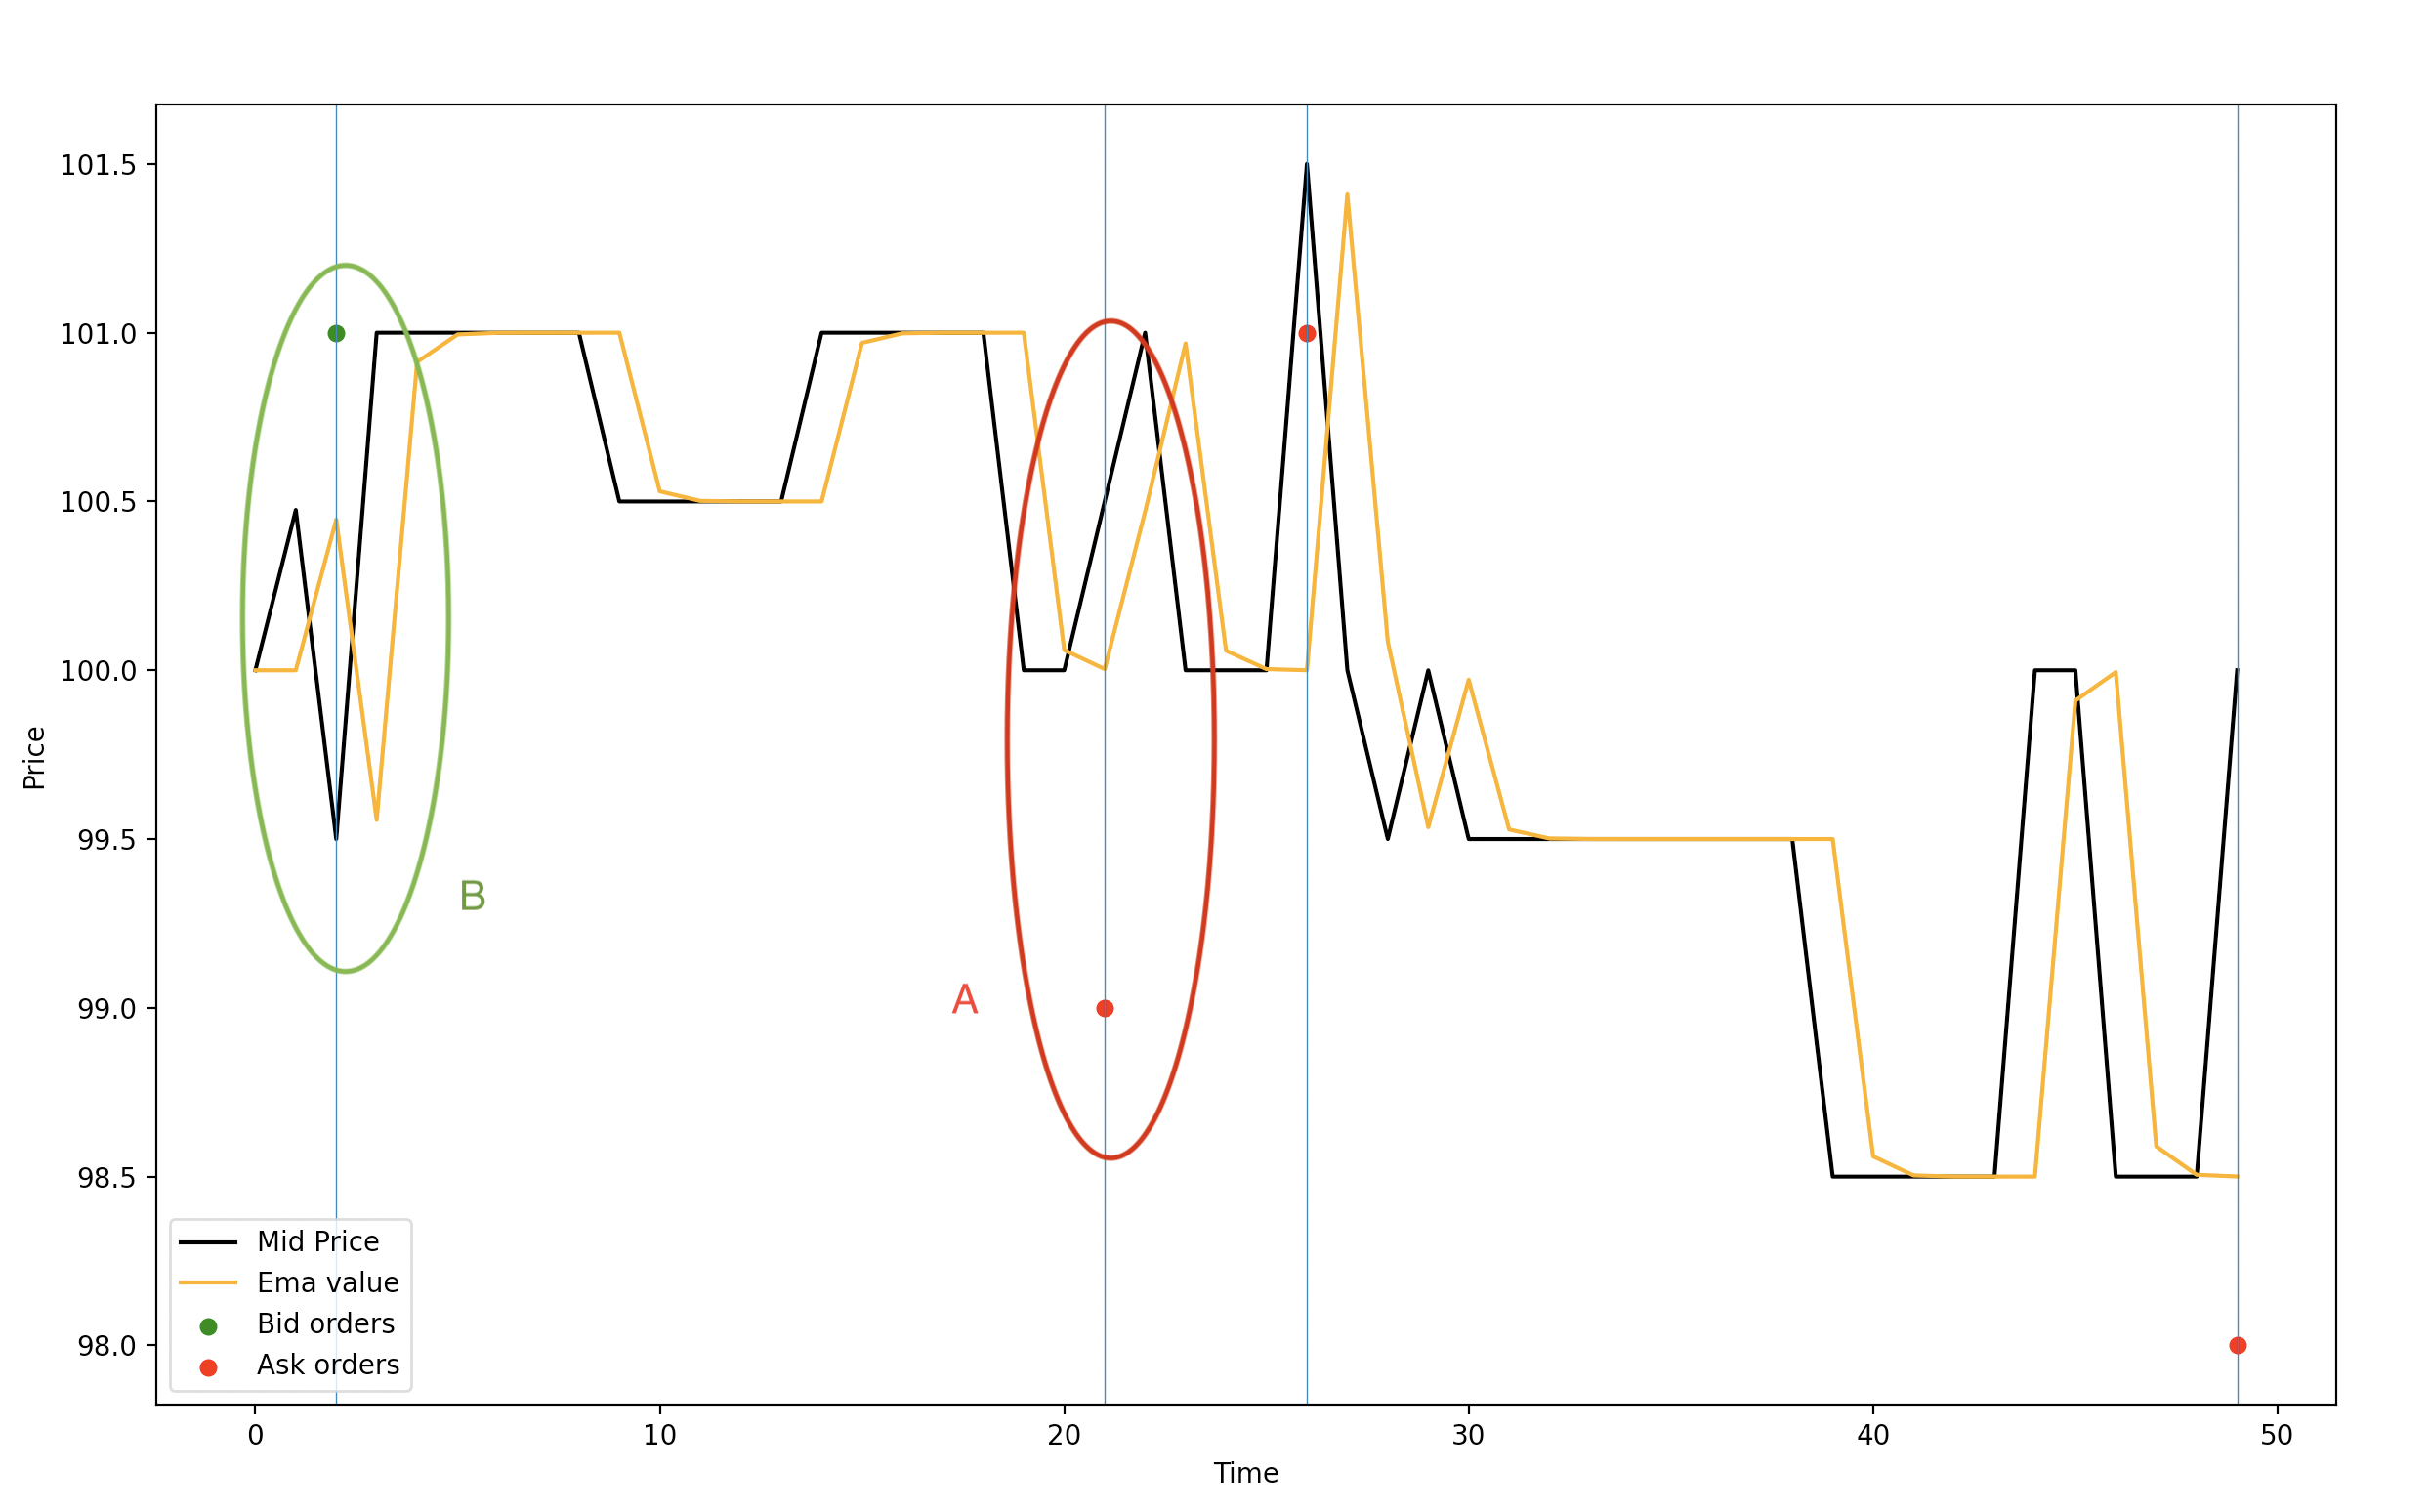
\includegraphics[ height=8cm]{Dissertation/images/mcg_indv/MEAN_R/sample.png}
\caption{Simple Agents and Mean reversion trader Experiment} 
\label{fig:MR_first_test}
\end{figure} 
\FloatBarrier

The behaviour of the Mean reversion trader can be illustrated by the three points depicted in Figure \ref{fig:MR_first_test}. 
\begin{itemize}
  \item \textbf{A} : This depict a point where the $ema_{t}$ value is below the mid price. This means that the mean reversion trader will submit an ask order because it believes that the price will eventually go down or return to the moving average. The red dot at the lower peak of the point illustrates an ask order submitted at the best ask price. This illustrates the first condition of the algorithm 4.4. We have that the $ema_{t}$ is 100 and $p_t$ is 100.5. Given that $ema_t \leq p_t$ and $k$ is 1 and the standard deviation at time t is 0.47, $0.5 \ge 1 * 0.47$, which is why the agent submitted a sell order.
  
  \item \textbf{B} : This depict a point where the $ema_{t}$ value is above the mid price. This means that the mean reversion trader will submit a bid order because it believes that the price will eventually go up back to the moving average. The green dot at the top of the point illustrates a bid order submitted at the best bid price. This illustrates the second condition of the algorithm 4.4. We have that the $ema_{t}$ is 100.5 and mid price is 99.5. The standard deviation at time t is 0.5. Given that $ema_t \ge p_t$ and and $k = 1$, we have that $1.0 \ge 0.5$, hence the agent submitted a buy order. 
  
\end{itemize}

However, this also represents a problem. The $ema_{t}$ line is not similar to what is commonly see in other literature. We have decided to test another ema equation. 

\begin{equation}
ema_t = (p_{t} - ema_{t-1}) * (2 / n + 1) + ema_{t-1} 
\end{equation}
where n = period.

If the McG value of 0.94 is calculated using this equation, then the period would be 1.1, which is the same as taking only the previous value into account. However, with the new equation, the coefficient will be 0.04, which is much less than the value specified in McG paper. 

\begin{figure}[h]
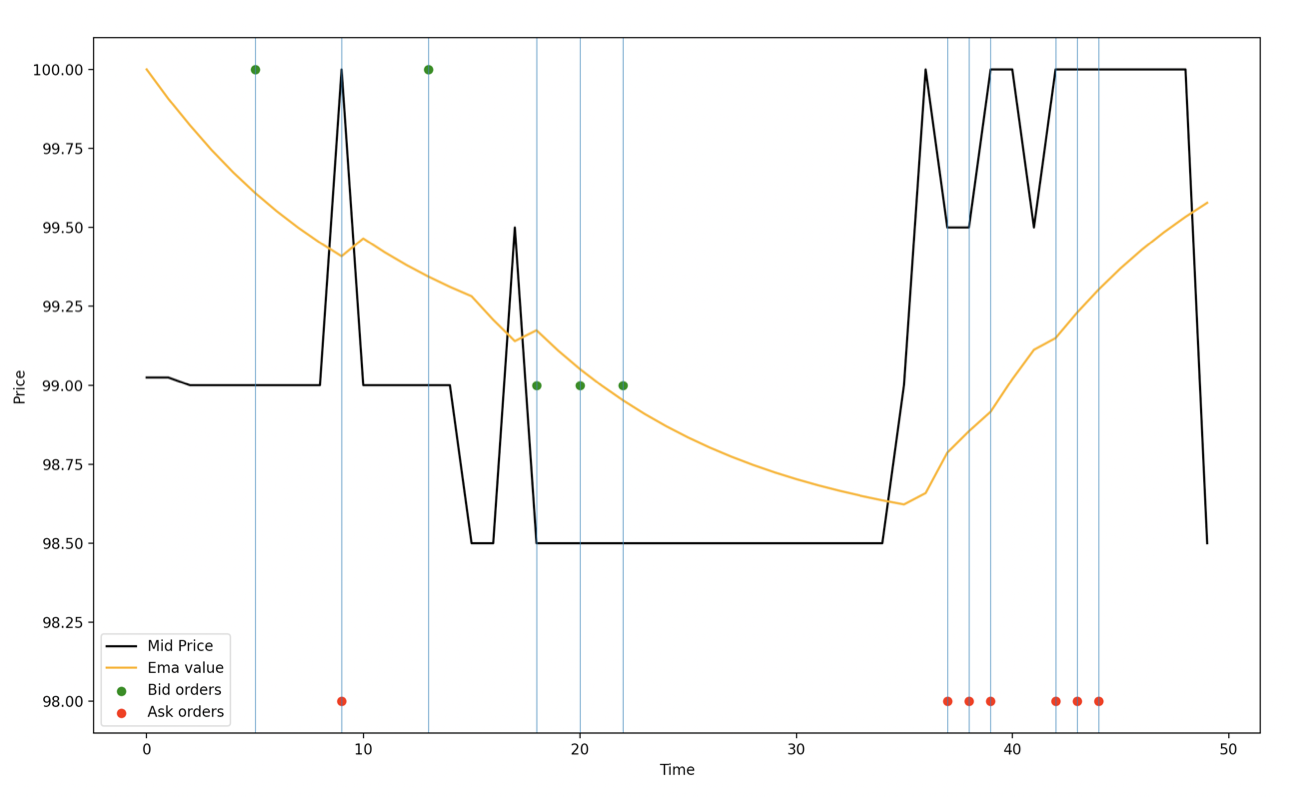
\includegraphics[ height=8cm]{Dissertation/images/mcg_indv/MEAN_R/online.png}
\caption{Simple Agents and Mean reversion trader Experiment} 
\label{fig:MR_online}
\end{figure} 
\FloatBarrier

Figure \ref{fig:MR_online} illustrates the same experiment with the new $ema_t$ equation. The Mean reversion agent still submits the orders in the same behaviour but the $ema_t$ line is much similar to that of other literature. 

\section{Noise trader} 
The Noise trade is also based on Cui and Barbazon \cite{CuiNoise} conference paper. Cui and Barbazon main objective was to examine wheter intelligence in a trading agent is needed to mimic the price impact and size of order relationship, which is why they implemented the Noise trader in order to replicate the statistics seen in real financial exchange. This is why the  Noise trader is defined so that it can captures other activities in the financial market since its parameters are based on real market data. It randomly execute a sell or a buy with equal probability. Once decided, the agent either place a market order or limit order or cancel existing order with probability $\lambda_{m}$, $\lambda_{l}$ and $\lambda_{c}$ respectively. If it does submit an order, the volume is drawn from a log-normal distribution described by:
\begin{equation}
v_t = exp(\mu + \sigma u_v) 
\end{equation}
where $\mu$ and $\sigma$ is mean and standard deviation of the $v_{ts}$ natural logarithm. $u_v$ is a value uniformly drawn between 0 and 1. Two other conditions of the Noise trader is as follow: 

\begin{itemize}
    \item Noise trader's market orders quantity cannot be more than half of the opposite side of the book
    \item Noise trader must make sure no side of the book is empty and submit limit orders accordingly
\end{itemize}
\begin{algorithm}[H]
\DontPrintSemicolon 
\If{$random() < \delta_{nt}$} {

    \If{$random() < 0.5$} {
    Decides to Sell\;
    }
    \Else{
    Decides to Buy;\
    }
    \EndIf
    Generate $U(0,1)$ to determine action,$\lambda_{m}$ , $\lambda_{l}$ and $\lambda_{c}$.
    
    \Switch{action}
    {
        \Case{Submit Market Order with probability $\lambda_{m}$ }{Submit market order with volume calculated by $v_{nt} = exp(\mu + \sigma u_v)$}
        \Case{Submit Limit Order with probability $\lambda_{l}$}{
        Generate $U(0,1)$ to determine action,$\lambda_{crs}$ , $\lambda_{inspr}$,$\lambda_{spr}$  and $\lambda_{cspr}$.
            \tcc{The condition of these cases are such that $\lambda_{crs} + \lambda_{inspr} + \lambda_{spr} + \lambda_{offspr} = 1$. }
            \Switch{action}
            {
                \Case{Crossing Limit Order with probability $\lambda_{crs}$ }{Submit limit order at opposing best price with volume $v_{nt}$ }
                \Case{Inside spread limit order with probability $\lambda_{inspr}$ }{Generate random value with $U(BestBid,BestAsk)$ with volume $v_{nt}$}
                \Case{Spread Limit Order with probability $\lambda_{spr}$ }{Submit limit order at the best price with volume $v_{nt}$}
                \Case{Off-spread Limit Order with probability $\lambda_{offspr}$ }{Generate a random price value using $xmin_{offspr} * (1-u_0)^{-\frac{1}{\beta - 1}}$ with volume $v_{nt}$ }
            
            }
        }
        \Case{Cancel Existing Order with probability $\lambda_{c}$ }{Cancel the oldest order previously submitted.}
    }
  }
\EndIf
\caption{{\sc Noise trader reproduced from McG (4.5) \cite{McGroarty}} }
\end{algorithm}

\begin{table}[h]
\centering
\begin{tabular}{ |m||p{4cm}|} 
\hline
\textbf{Noise Trader Parameters}& \textbf{Value} \\
\hline
\hline
buy or sell & $ p_{action} = 0.5 $ \\ 
\hline
Market order probability & $\lambda_{m}$ = 0.03\\ 
\hline
Limit order probability & $\lambda_{l}$ = 0.54\\ 
\hline
Cancel order probability & $\lamda_{c}$ = 0.43\\
\hline 
Market order quantity & $\mu_{mo} = 7 \sigma_{mo} = 0.1 $\\
\hline
Limit Order quantity &  $\mu_{lo} = 8 \sigma_{lo} = 0.7 $\\
\hline
Off-spread relative price & $xmin_{offspr} =0.005$
\newline 
$\beta_{offspr} = 2.72 $\\
\hline
\textbf{Limit order types} & \\
\hline
Crossing limit order & $\lamda_{crs} = 0.003$\\
\hline 
Inside-spread Limit order & $\lamda_{inspr} = 0.098$\\
\hline 
Spread Limit order & $\lamda_{spr} = 0.173$\\
\hline 
Off-spread Limit order & $\lamda_{offspr} = 0.726$\\
\hline
\end{tabular}
\caption{Noise trader parameters taken from \cite{McGroarty}}
\end{table}
\FloatBarrier 

The Noise trader is intended to represent other forms of behaviour in the market. By looking at the parameters of the Noise trader, it is clear that the Noise agent will mostly either submit a limit order or cancel an order. By taking a closer look at the limit order, the agent will mostly submit an Off-spread limit order. According to Cui and Barbazon \cite{CuiNoise}, the Off-spread price of the order is given by the $BestBid - RP_{offspr}$ in a bid order and $BestAsk + RP_{offspr}$ in an ask order. The value $RP_{offspr}$ is given by $xmin_{offspr} * (1-u_0)^{-\frac{1}{\beta - 1}}$. This is equivalent to the price below the Best Bid and above the Best Ask.

By looking the values of the $RP_{offspr}$, one can predict what the range of the price submitted can be. 

\begin{table}[h]
\centering
\begin{tabular}{ |m||p{4cm}|} 
\hline
\textbf{Uniform random value $u_0$}& \textbf{$RP_{offspr}$ Value} \\
\hline
\hline
0 & 0.5\\
\hline 
0.1 & 0.5\\
\hline 
0.2 & 0.4\\
\hline 
0.3 & 0.4\\
\hline 
0.4 & 0.4\\
\hline 
0.5 & 0.3\\
\hline 
0.6 & 0.3\\
\hline 
0.7 & 0.2\\
\hline 
0.8 & 0.2\\
\hline 
0.9 & 0.1\\
\hline 
1.0 & 0.0\\
\hline
\end{tabular}
\caption{Noise trader parameters taken from \cite{McGroarty}}
\end{table}
\FloatBarrier 

Table 4.6 of $RP_{offspr}$ calculations illustrates how the values of the off-spr price should not vary much from the initial price. Figure \ref{fig:Noise_test_mp} below illustrates that price that the Noise trader submits within a market of homogeneous 6 Noise agents running with 3000 McG time-period or ten-percent of the whole run-time. The initial price is 100 and the spread is 0.5. 

\begin{figure}[!htbp]
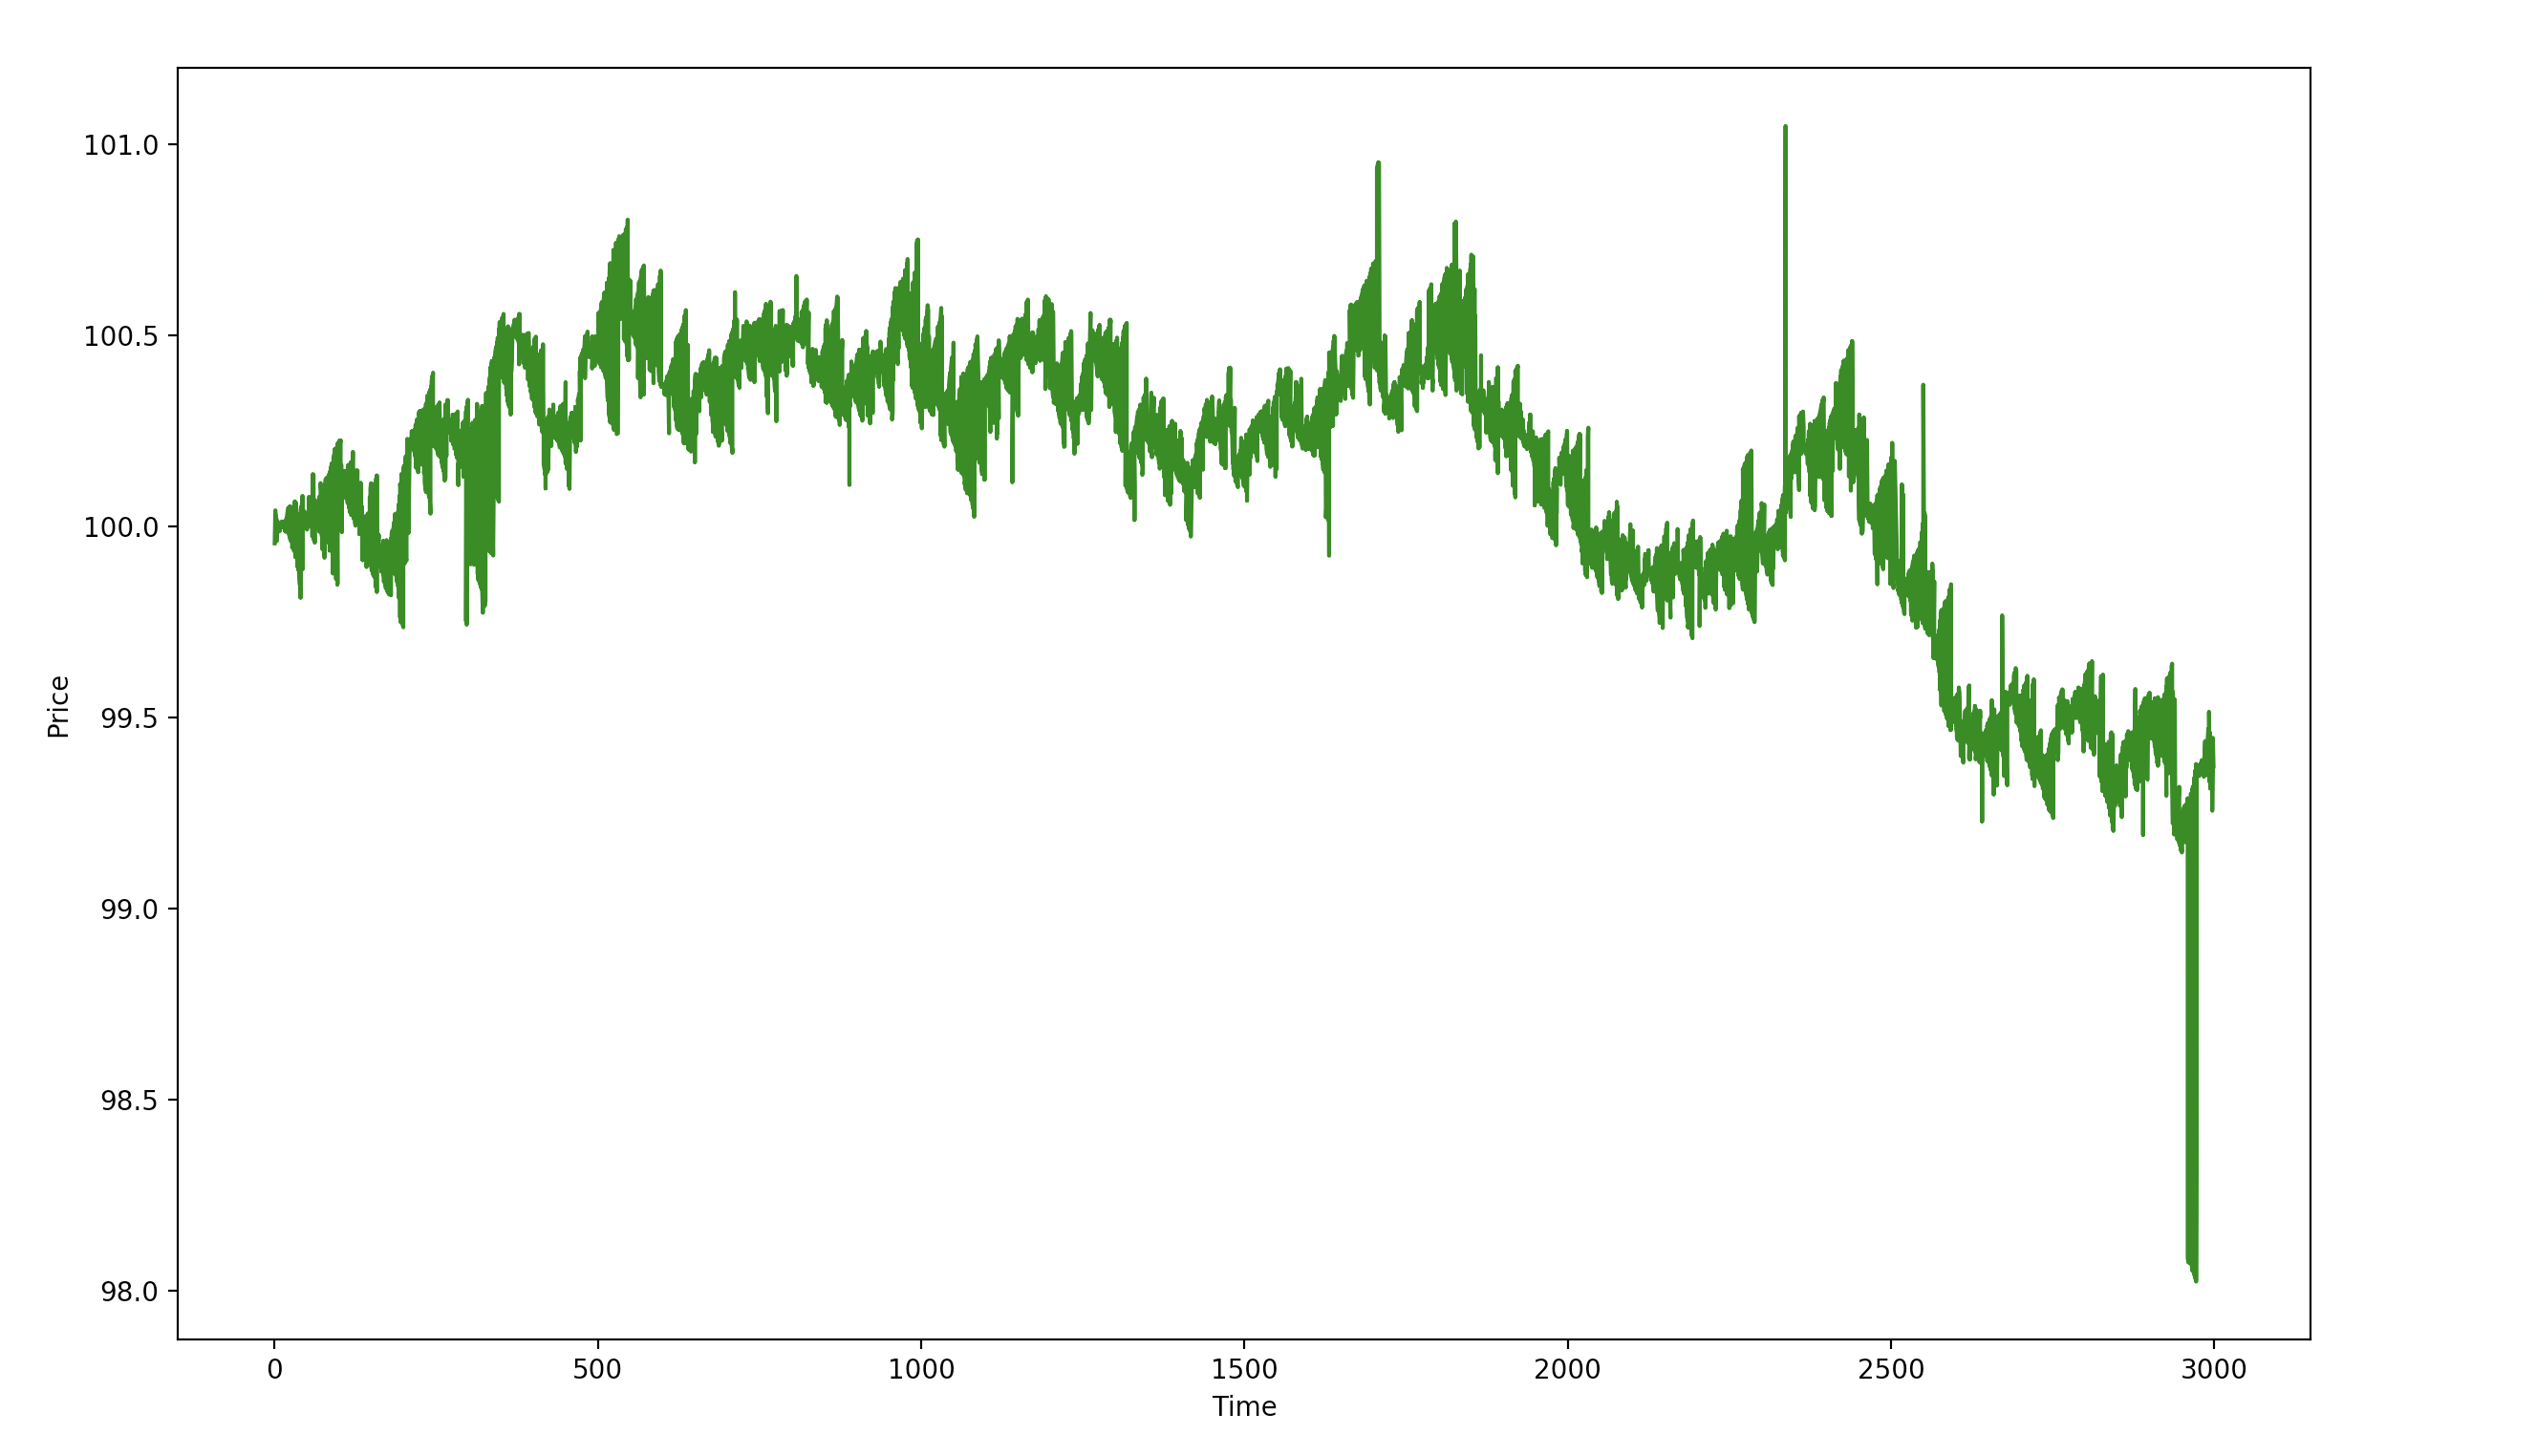
\includegraphics[ height=8cm]{Dissertation/images/mcg_indv/Screenshot 2020-03-20 at 14.33.18.png}
\caption{Noise trader order price} 
\label{fig:Noise_test_mp}
\end{figure} 
\FloatBarrier

 
As expected, the price is hugely volatile, due to the random variable of the off-spread price and inside spread limit order. However, the range is still near the initial price and gradually decreases due to the sudden decrease by 0.5 from the off-spr price, which is what can be expected. 

\subsection{Limit Order prices}
In this section, the purpose is do demonstrate the price ranges that the Noise trader will submit in its limit orders.

\begin{algorithm}[H]
\DontPrintSemicolon 
\Switch{action}
            {
                \Case{Crossing Limit Order }{Submit limit order at opposing best price with volume $v_nt$ }
                \Case{Inside spread limit order }{Generate random value with $U(BestBid,BestAsk)$ with volume $v_nt$}
                \Case{Spread Limit Order }{Submit limit order at the best price with volume $v_nt$}
                \Case{Off-spread Limit Order }{Generate a random price value using $xmin_{offspr} * (1-u_0)^{-\frac{1}{\beta - 1}}$ }
            
            }
\caption{{\sc Noise trader Limit order algorithm reproduced from McG (4.5) \cite{McGroarty}}}
\end{algorithm}

In this experiment, the market will consist of 10 Noise traders, running for 30,000 McG time-step to demonstrate the price ranges. For simplicity, we will set the best ask to 299 and best bid to 301 in order to see the variations in order prices and not the best prices itself. The results are given below. 

\begin{table}[h]
\centering
\begin{tabular}{ |l||l|l|l|} 
\hline
\textbf{Order type}& \textbf{Probability} & \textbf{Min value} & \textbf{Max value} \\
\hline
\hline
Crossing Limit order & 0.003 & 299 & 301 \\ 
\hline
Inside spread Limit order & 0.098 & 299 & 300.99 \\ 
\hline
Spread Limit order & 0.173 & 299 & 301 \\ 
\hline
Off-spread Limit order & 0.726 & 299.00& 300.99 \\ 
\hline
\end{tabular}
\caption{Number of transactions in each implementation}  
\end{table}
\FloatBarrier

The Cross limit order, Inside spread limit order, Off-spread limit order and Spread limit order must be inside the best ask and best bid range, which in this case, it is. 

\subsection{Order types submitted overall}

In this section, the purpose is to explored how many orders are actually submitted by the Noise trader and to prove that the types of orders submitted lines up with the initial parameter of the Noise trader. 

\begin{table}[h]
\centering
\begin{tabular}{ |l||l|p{2cm}|p{6cm}|} 
\hline
\textbf{Order types} & \textbf{Probability} & \textbf{Value from Experiment} & \textbf{Rough sketch of calculation} \\
\hline
\hline
Ask order & 0.5 & 4877 & $(9284 + 554) / 2 = 4919 \approx 4877$\\ 
\hline
Bid order & 0.5 & 4961 & $(9284 + 554) / 2 = 4919 \approx 4919$\\ 
\hline
\hline
Market order & 0.03 & 554 & $(9284 + 554 + 8162) * 0.03 = 540 \approx 554$\\ 
\hline
\hline
Limit order & 0.54 & 9284 & $(9284 + 554 + 8162) * 0.54 = 9720$  
\newline $\approx 9284 $\\ 
\hline
Crossing Limit Order & 0.003 & 26 & $9284 * 0.003 = 28 \approx 26 $\\ 
\hline
Inside-spread Limit Order & 0.098 & 901 & $9284 * 0.098 = 909 \approx 901 $\\ 
\hline
Spread Limit Order & 0.173 & 1709 & $9284 * 0.173 = 1606 \approx 1709 $\\ 
\hline
Off-spread Limit Order & 0.726 & 6648 & $9284 * 0.726 = 6740 \approx 6648 $\\ 
\hline
\hline
Cancel existing order & 0.43 & 8162 & $(9284 + 554 + 8162) * 0.43 = 7740  \approx 8162 $\\ 
\hline
\end{tabular}
\caption{Noise trader experiment statistics} 
\end{table}
\FloatBarrier 

In most cases, the results line up with the statistics shown as well as the proportion of the orders types submitted.

\section{Evaluation}
This chapter provides us with a deeper insight and parameters exploration that will aide us in the market experiments in the next chapters. Overall, the agents are functioning properly and the behaviour of the agents matches what is described in McG. This means that the next step of the project is to look at how these agents behave when they act in the same market and what are the characteristics of the market which mimics that of real financial exchange market dynamics. We will first investigate the same configuration as Oesch to ensure that three out of five agents are functioning in an appropriate manner before moving to two of the remaining agents. 

\chapter{Oesch experiment results} 
As the behaviour of each individual agent has been described and tested, the next step is looking at a market consisting of some or all of the agents. This has been described in both Oesch 2014 \cite{Oesch} and McG \cite{McGroarty} papers. By comparing the results produced, one can confirm that the agents have been correctly implemented. 

\section{Oesch's Experiment}
\subsection{Oesch's Experiment configuration compared to McG}
McG claims that they have taken the Liquidity consumer and Market maker (Liquidity provider) from the Oesch paper. In addition, both papers referred to Wei and Barbazon \cite{CuiNoise} in Noise trader algorithm. Oesch provides an example result of running the three agents in the same market in addition to the mid price and return series graph. This is a great benchmark to compare whether the agents' behaviour is correct. If the results are similar, it can be concluded that at least three out of five agents are acting correctly when McG results are compared. 

Oesch has a different time step compared to the McG action-step. In each Oesch time-step, a group randomly and uniformly selected between Noise trader, Market maker and Liquidity consumer. Then an agent is selected randomly from the group. The probability of each agent being selected is as follow : 

\begin{table}[h]
\centering
\begin{tabular}{ |m||p{4cm}|} 
\hline
\textbf{Probability of each trader being selected}& \textbf{Value} \\
\hline
\hline
Market maker & 0.15 \\ 
\hline
Liquidity consumer & 0.05\\ 
\hline
Noise Trader & 0.8 \\ 
\hline
\end{tabular}
\caption{Momentum trader parameters taken from \cite{McGroarty}} 
\end{table}
\FloatBarrier 

Unlike McG, when an agent is chosen, it is required to act. The agent can either submit or cancel an order. An order submitted can either be limit order or market order. Other minor changes to the agent are as follow: 

\begin{itemize}
  \item \textbf{Liquidity consumer} : Instead of drawing only from a single large order, if the initial large order at the start of the day is empty, the agent will generate a new one and continue submitting market orders. 
  \item \textbf{Noise Trader} : parameter $xmin_{offspr}$ is 0.05 instead of 0.005. This means that the offspread price generated by the agent will have a higher range then the McG noise agent. 
\end{itemize}

\begin{figure}[h]
  \begin{subfigure}[b]{0.5\textwidth}
    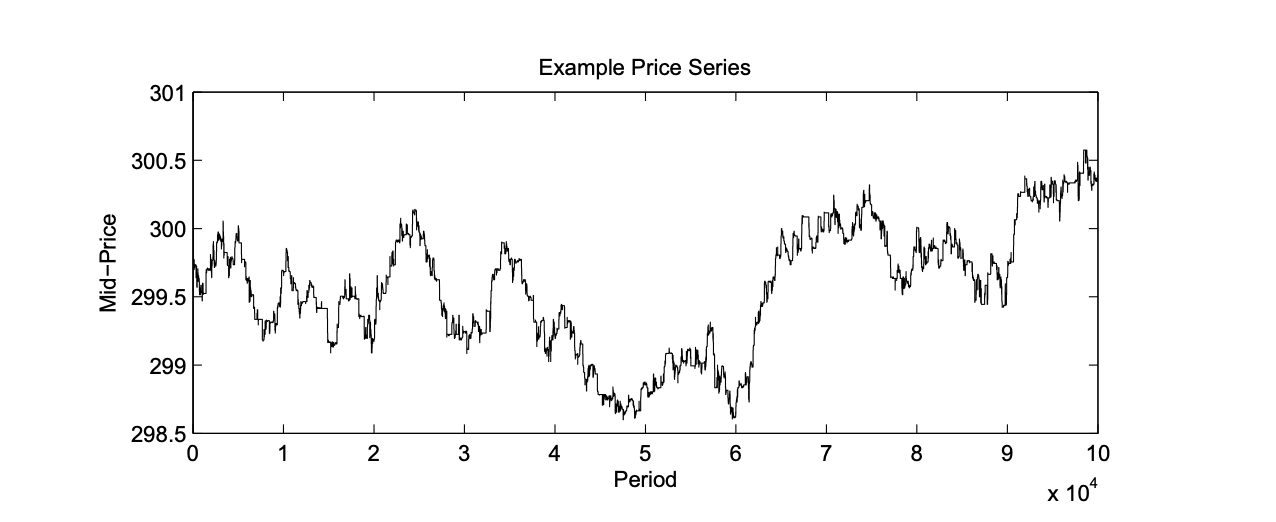
\includegraphics[width=8cm, height=7cm]{Dissertation/images/Market_experiment/Original_mp.png}
    \caption{Mid Price}
    \label{fig:1}
  \end{subfigure}
  %
  \begin{subfigure}[b]{0.5\textwidth}
    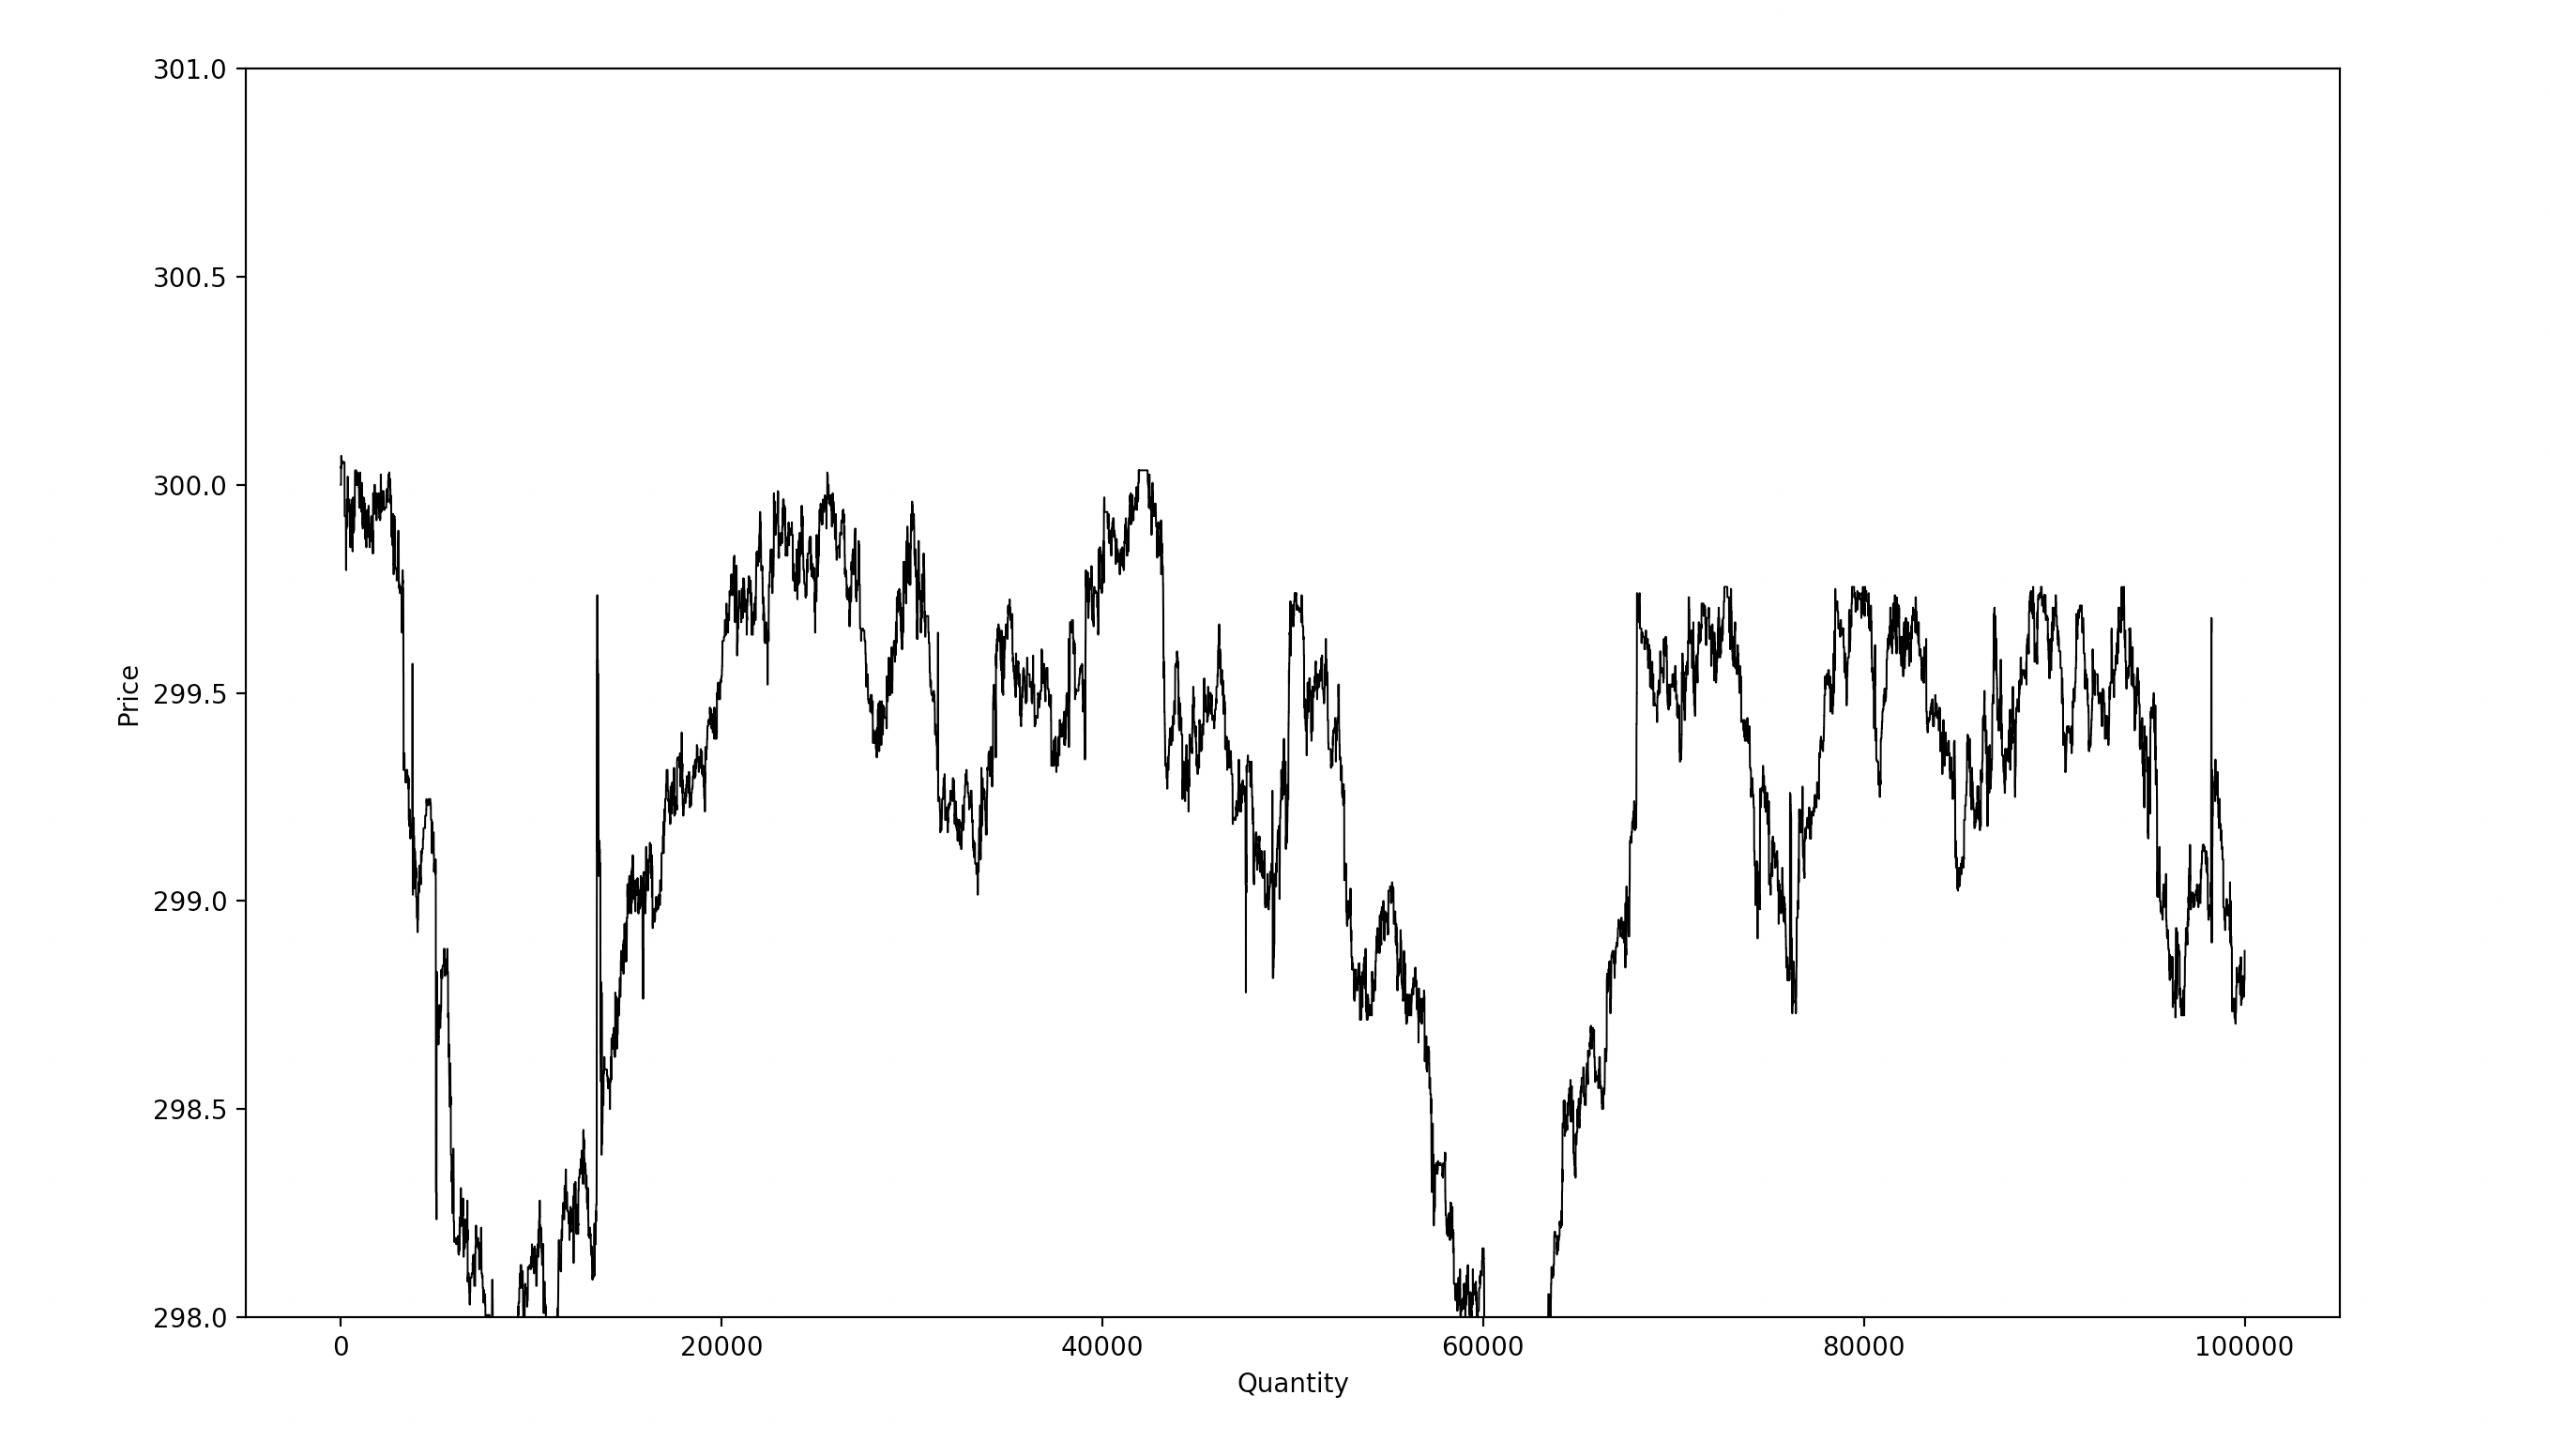
\includegraphics[width= 7cm, height=6cm]{Dissertation/images/Market_experiment/sample2_mp.png}
    \caption{Example Return Series (1 - y values)}
    \label{fig:2}
  \end{subfigure}
\caption{Replication of Oesch's experiments with similar configurations} 
\end{figure}

\begin{figure}[h]
  \begin{subfigure}[b]{0.5\textwidth}
    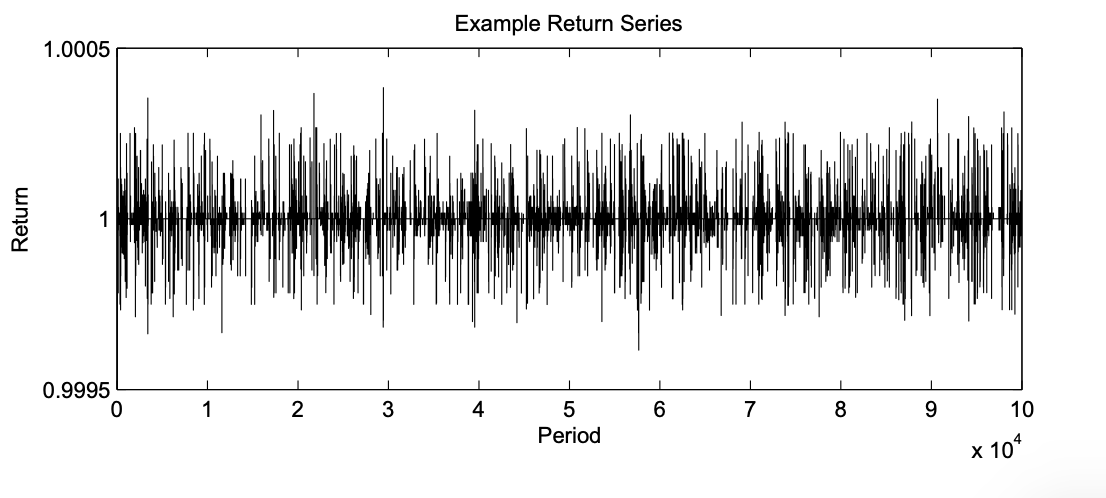
\includegraphics[width=7cm, height=6cm]{Dissertation/images/Market_experiment/Original_return.png}
    \caption{Mid Price}
    \label{fig:1}
  \end{subfigure}
  %
  \begin{subfigure}[b]{0.5\textwidth}
    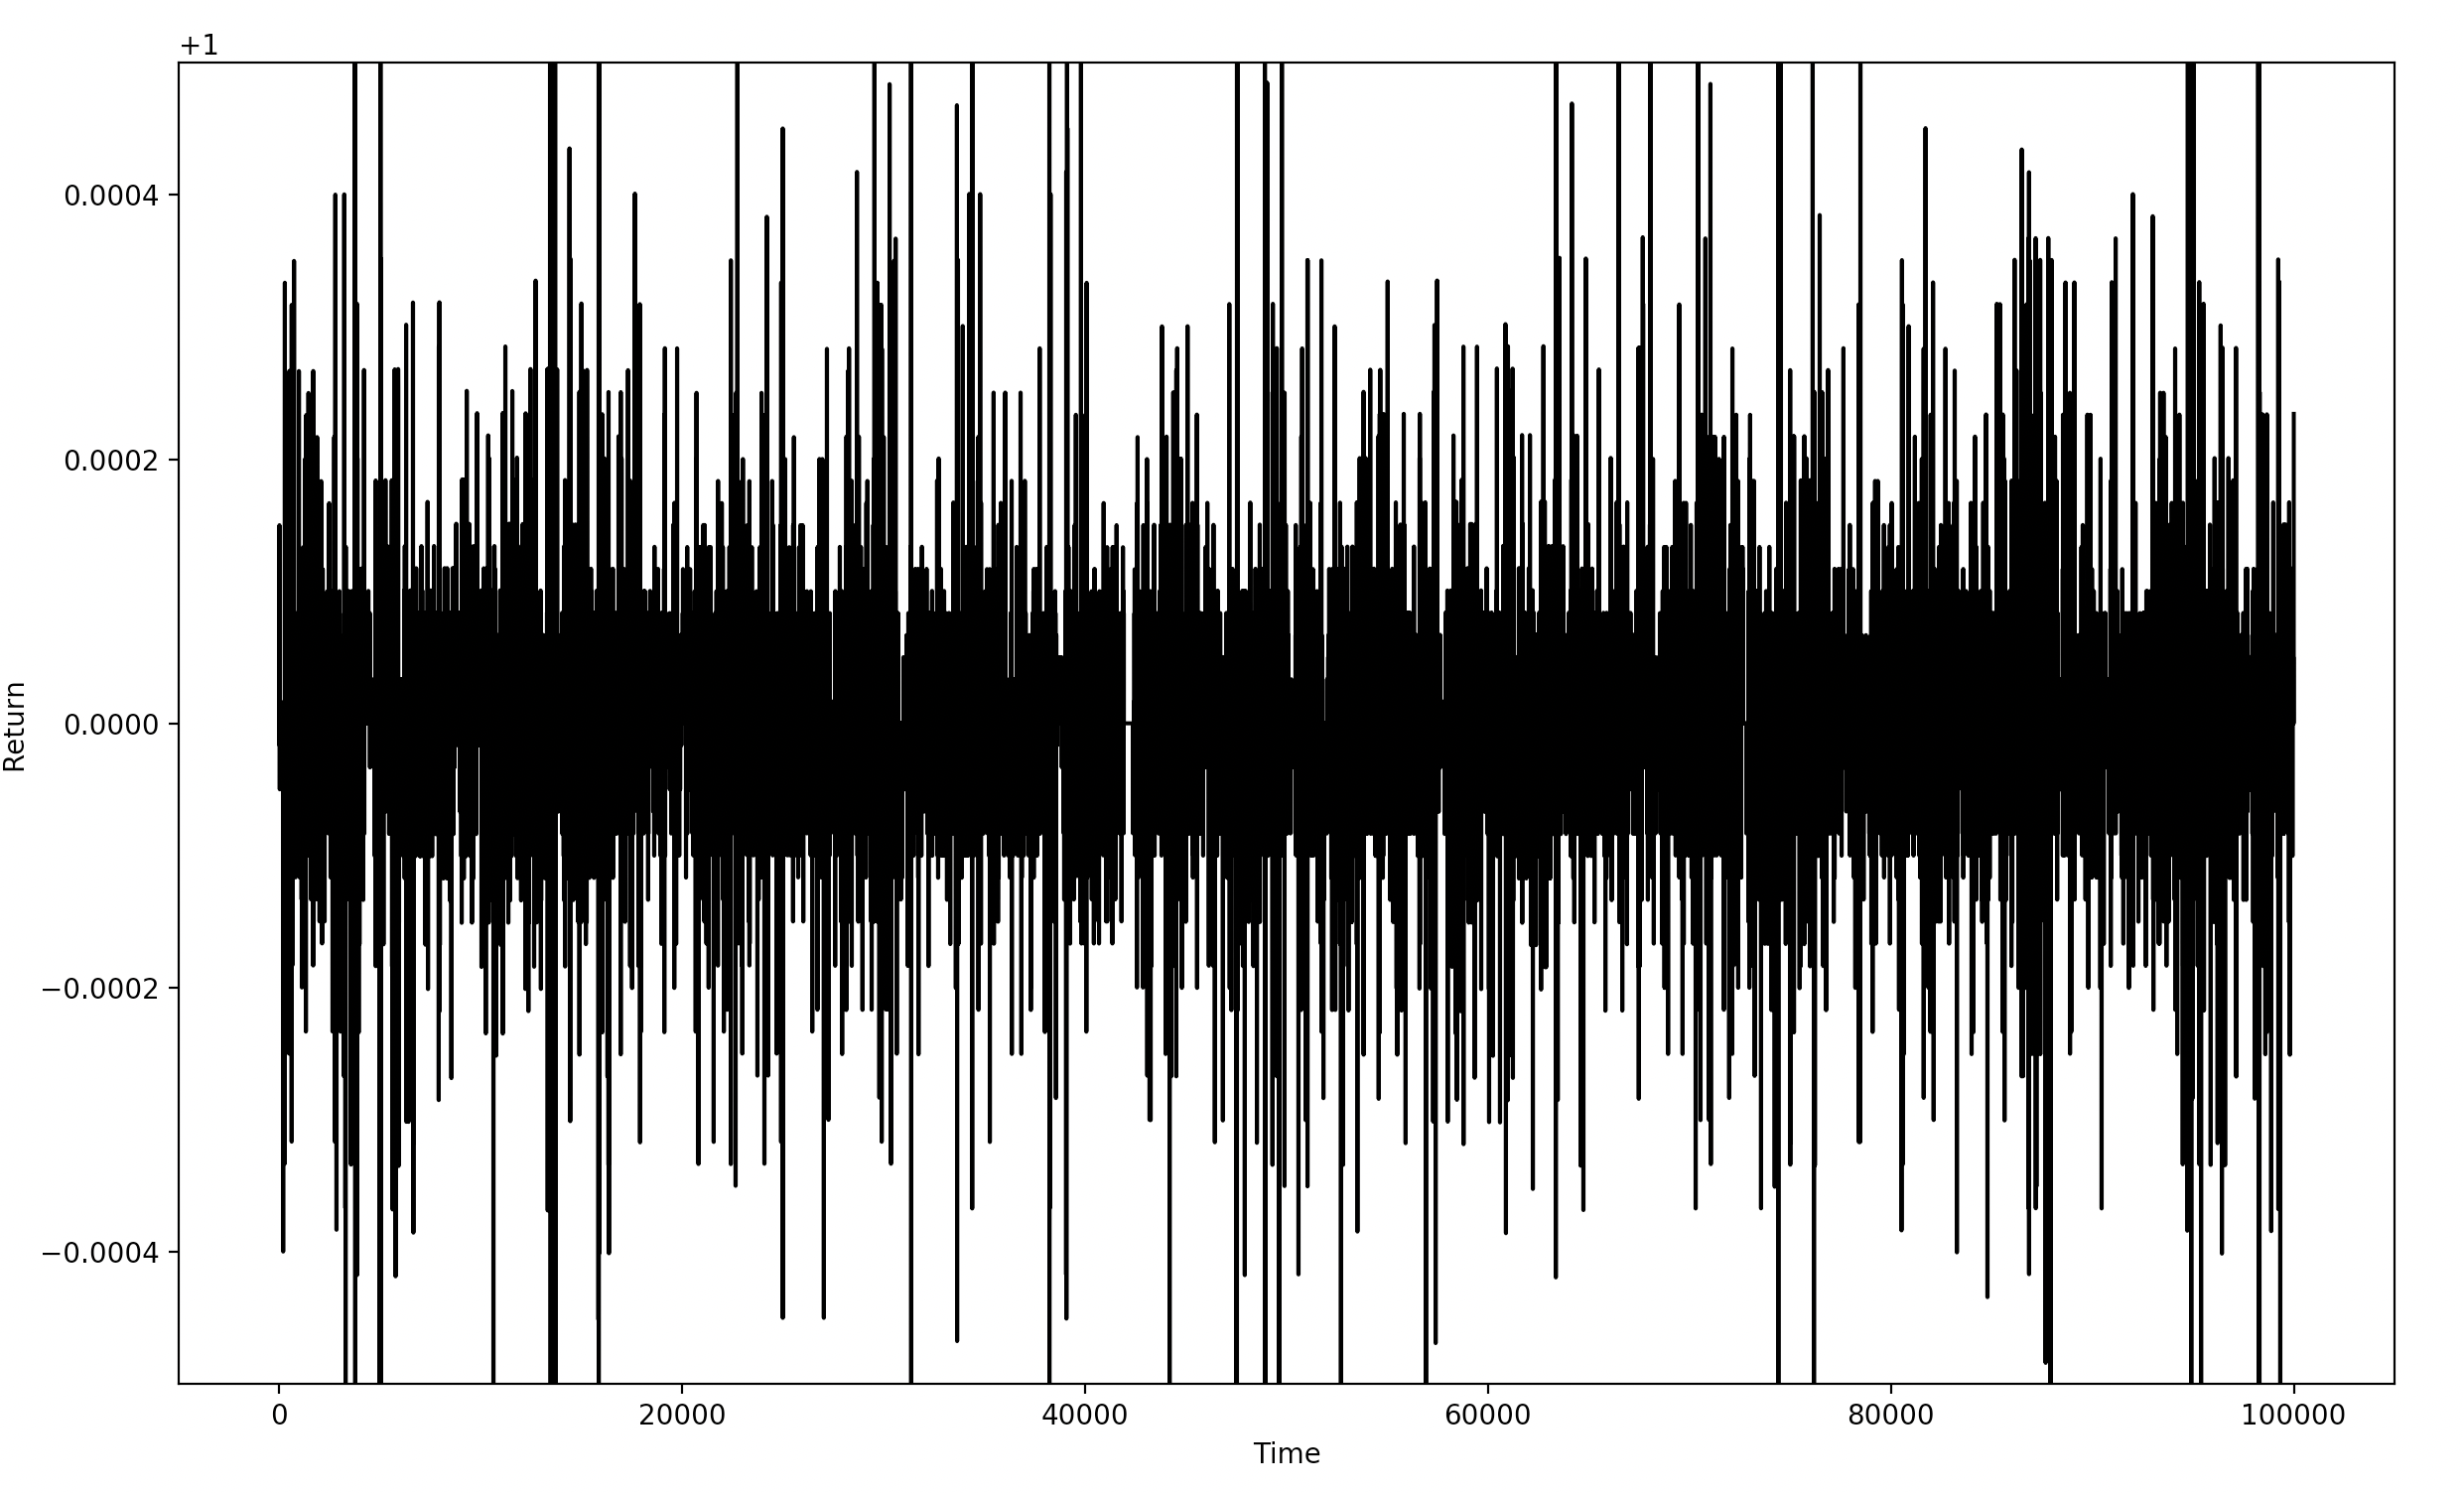
\includegraphics[width= 7cm, height=6cm]{Dissertation/images/Market_experiment/sample2_return.png}
    \caption{Example Return Series (1 - y values)}
    \label{fig:2}
  \end{subfigure}
\caption{Replication of Oesch's experiments with similar configurations} 
\end{figure}

Figure 6.2 depicts the results after replication of Oesch's experiment. The market consists of 40 of each trader. The mid price value is still in range of the original experiment, which is between 298.5 and 301. The price movement exhibits similar movements over the period of time. There are some important factors that contribute to why the results may not be totally similar. 

\begin{itemize}
  \item Oesch's results in mid price and return series does not state how many or what is the ratio of the agent types in the market when the experiment is being conducted.
  \item The details of the agents are all explained verbally, which may not be as detailed as the one described in McG with clear algorithm. There are obvious difference between the agents in the two papers and the difference in results can be correlated with the missing details of the agents in Oesch's. 
\end{itemize}

\chapter{McG experiment results} 
\section{McG Experiment Result} 
In this section, we will discuss the results from running the market in full McG action-step system with all the agents. Similar to Oesch, McG does not fully state the ratio of the agents nor the number in each run. McG only reported their results as return statistics and price spikes data. In addition, because of hardware limitation and time-constraint, we will only be testing the McG experiment with 100,000 maximum time-step since running 300,000 takes at least 7 hours on our personal computer and the increase in time-period does not change the market dynamics. 

\subsection{Changes to Mean reversion and Momentum traders}
Upon investigation, the Mean reversion and Momentum trader seems to be submitting less than ideal orders and quantity of the orders compared to the other agents. In a 30,000 action-step in testing, the agents occasionally submit lower than 10,000 quantity or does not submit any orders at all. This means that some changes needed to be made to the agents in order to adapt them to the market. 

\begin{table}[h]
\centering
\begin{tabular}{ |m||p{4cm}|p{4cm}|} 
\hline
\textbf{Agent Parameter}& \textbf{ Original Value } & \textbf{New Value} \\
\hline
\hline
Momentum Trader's Wealth $W_{a,t}$ & 500,000 & 1,000,000  \\ 
\hline
Mean Reversion quantity per order $V_{mr}$ & 1 & $U(1, 5000)$ \\ 
\hline
\end{tabular}
\label{Tab:C5_parameters}
\caption{Changes in parameters of Mean Reversion trader and Momentum trader}  
\end{table}
\FloatBarrier

Because McG does not specify how to calculate the wealth of the Momentum trader, a choice has to be made regarding its initial wealth. In a 10,000 action-step, 500,000 worked well with the initial test since the total time period is smaller. However, since the current time period is higher, the wealth has to be increase in order to make the agent participate for the whole period without losing much of its wealth as well as submitting an increasing quantity of orders. 

For the Mean reversion trader, the quantity described by McG does not make sense since other agents are submitting more than 1 orders in most cases. The new change specifies that the Mean reversion trader will submit an order quantity uniformly distributed from 1 to 5,000. This number is taken from the average quantity that change make a shift of 0.05\% of mid price. A small experiment is conducted where a market of all five agents ran and recorded a shift in price when an order is submitted of more than 0.05\% from the initial price. The average of quantity of said order is 5,000. 

This change is crucial because in the next section where \textbf{Price Spike} is explained, the two agents, Mean reversion and Momentum trader will have an opposite behaviour in terms of types of orders submitted compared to one another. Hence, it does not make sense in this case where one will submit large quantities in an order while the other only submits orders of one quantity. 

In addition, McG specifies that Mean reversion agent has an effect on the mid-price and quantity of one is far too small to have an effect. Another possible change is to increase the number of Mean reversion agents in order to make the their orders have a larger effect on the market. 

The reason why these agents need to have a larger effect on the market is because McG market has a special property that mimics the real market dynamic called \textbf{Price Spikes}.

\subsection{Price Spike}

Taken from Johnson et al., McG describes a price spike as ``an occurrence of a stock price ticking down [up] at least ten times before ticking up [down] and with a price change exceeding 0.8\% of the initial price" \cite{McGroarty} McG claims that a Price Spike can occur when an agent ``eats through" the best price of one side of a book, causing a change in the mid-price of the market. This creates an upward or downward curve. Because there is a change in the mid-price, Momentum traders will now submit on the same side of the book, which pushes the price down the same direction. Mean Reversion trader, on the other hand, will detect a change in the mid-price and expects the price to shift back to its original moving average, hence will submit on the opposite side of the book. This means that there will be now roughly equal number of bids and sells which will stabilizes the mid price up to a certain point and stop the price from moving in the original direction. At this point, the Momentum trader may run no longer detect a large ROC and stop submitting. In addition, there will be another trader which will eat through the new higher or lower best price, causing a shift in the opposite direction of the original shift in price. 

\begin{figure}[h]
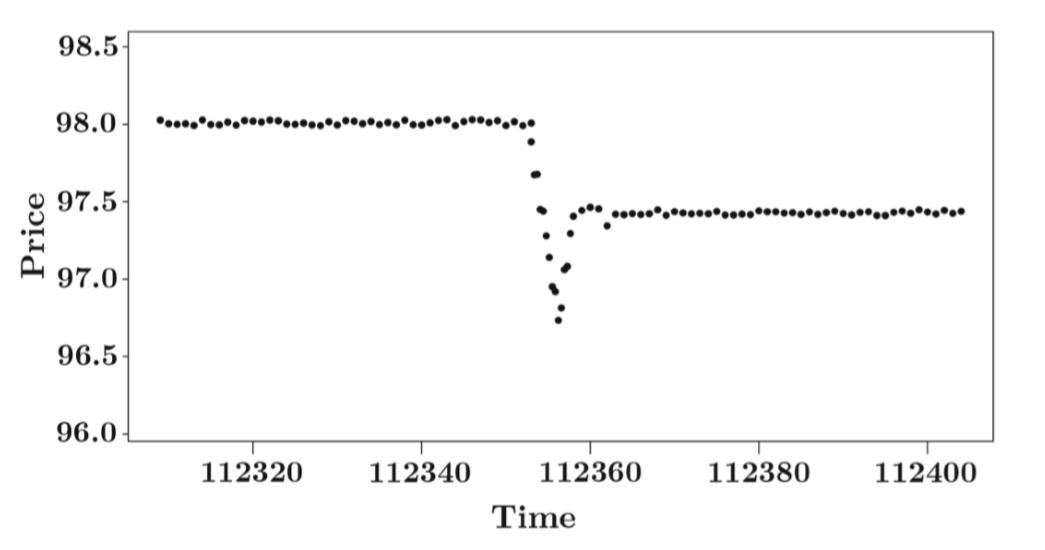
\includegraphics[ height=8cm]{Dissertation/images/Mcg_final/price_spike.PNG}
\caption{Price Spike example from \cite{McGroarty}}  
\end{figure} 
\FloatBarrier

In the current configuration, we were not able to detect a price-spike but there are other minor events which will be called \textbf{Minor Price Spikes} that exhibits the behaviour and relationship between Mean Reverison trader and Momentum trader. 

\subsection{Minor Price Spike}

A minor price spike can be defined as follow : An occurrence of price ticking up or down at least 5 times  with the maximum price of the ticks exceeding 0.6\% of the initial price. The event must happen in more than 5 action-steps. 

An example is given below: 
\begin{figure}[h]
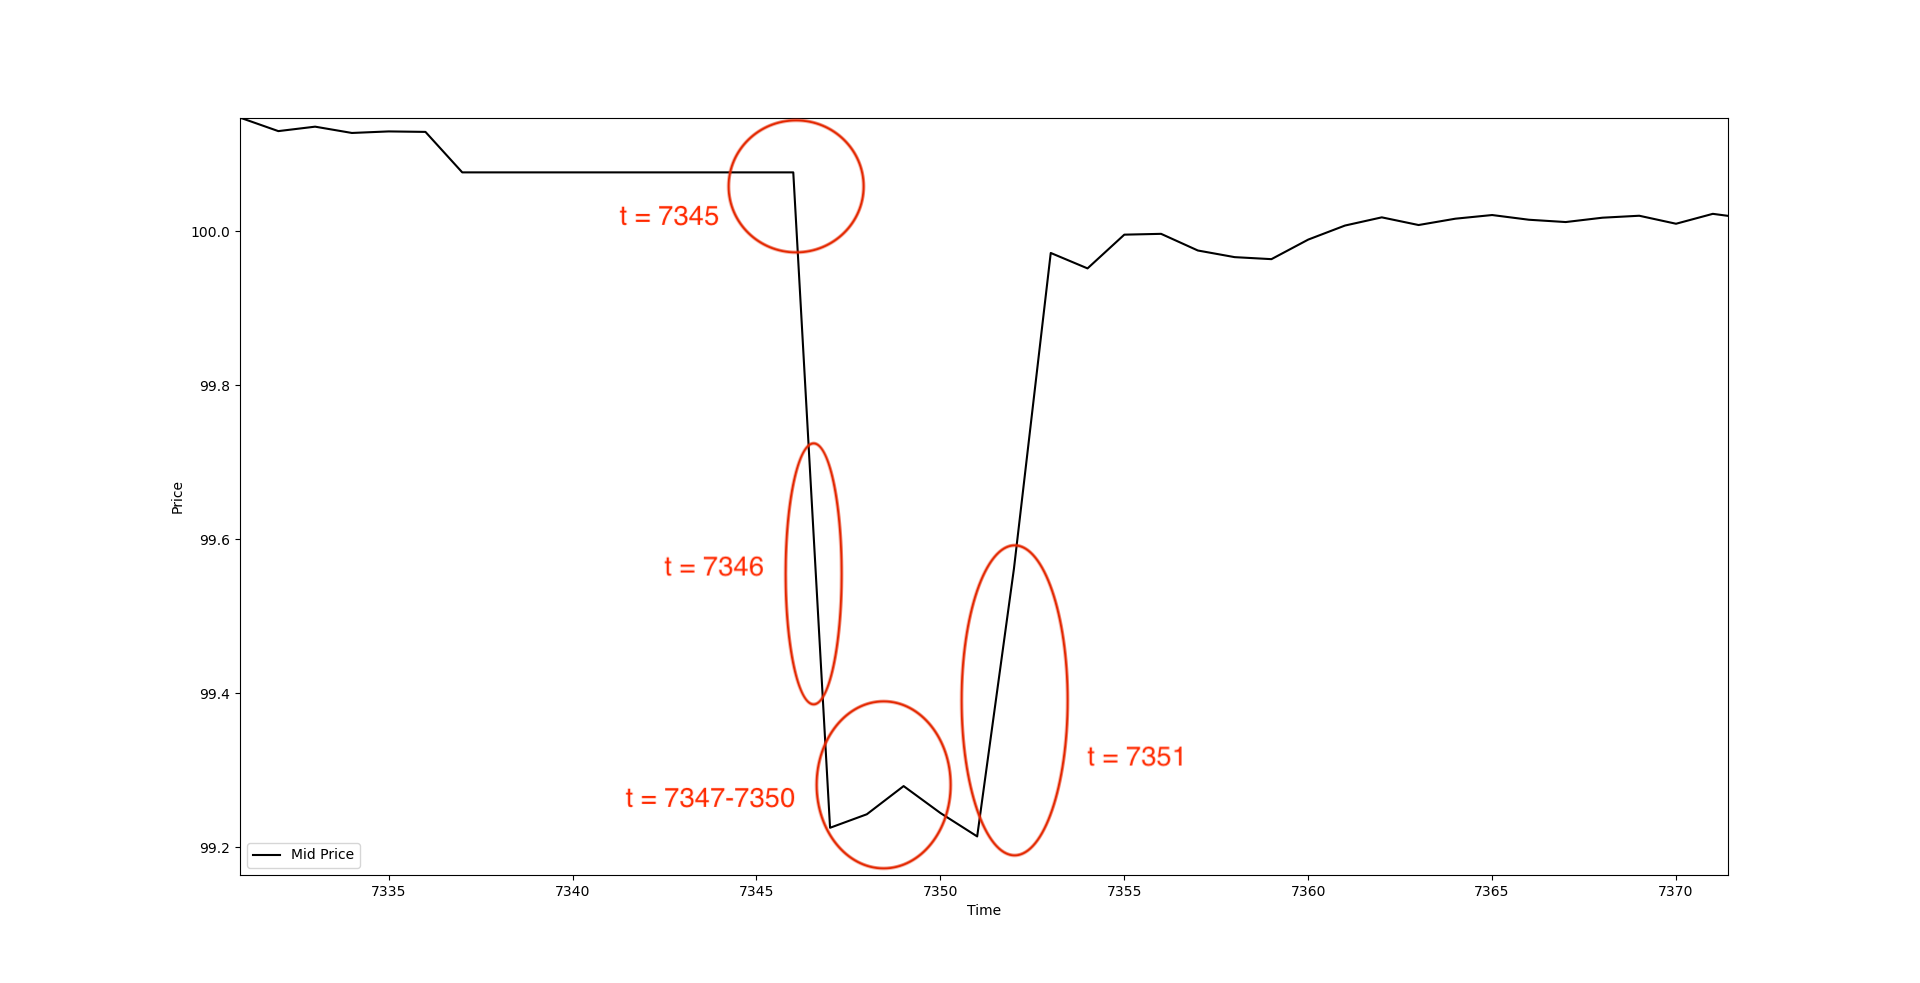
\includegraphics[ height=8cm]{Dissertation/images/Mcg_final/minor_spike_example.png}
\caption{Price spike example from the experiments}  
\end{figure} 
\FloatBarrier

A detailed explanation of the example spike: 
\begin{itemize}
  \item $ t = 7345$ A Market maker eats through the best price, causing the shift in the mid price of the market. 
  \item $ t = 7346 $ Mean reversion agents submits Bid orders while other agents, including Momentum trader, submit Ask orders causing the price to shift even downwards. Since there are more Ask order submitted, the price shifts downwards to 99.2. 
  \item $ t = 7347-7350 $ Mean reversion now submits an Ask order since the $ema_t$ value sees a small shift upward in price and because the McG value of 0.94 accounts to the change in the last 2 action-step price. However, the quantity is small since only a small portion of the agents are submitting. On the other hand, because there is still momentum from the last 5 action steps of a downward shift in price, the Momentum trader still submits Ask orders, but with less quantity, causing a smaller downward slope in the mid-price. 
  \item $ t = 7351 $ An agent again ``eats through" the best price, causing the mid price to shift upwards to 99.9. This causes the Momentum trader to submit bid orders while Mean reversion agent submits Ask orders. 
\end{itemize}

\section{Parameters and Minor Price Spike}
Now that there we have established the relationship between the Mean reversion and Momentum trader, the changes in parameter can also affect the number of minor spikes seen in the market. In this section, we will explore how the parameters of each trading agent, more specifically parameters that relate to their reaction to the market in terms of time-period and how these parameters effect the number of Minor Price Spikes found in each experiment. In addition, McG states in their paper that as the number of frequency trader increases, more price spikes can be seen \cite{McGroarty}. This can be shown with the number of Minor Price Spikes in our experiments, which will be illustrated in Table 6.4 below. 

\subsection{Threshold of Momentum trader and Number of Minor Price Spike recorded}

\begin{algorithm}[H]
\DontPrintSemicolon 
\If{$random() < \delta_{mt}$} {
    \If{$roc_t \ge \kappa$} {
    Submit market buy order with volume $v_t = \abs{roc_t} * W_{a,t}$\;
    }
    \uElseIf{$roc_t \leq -\kappa$}{
    Submit market sell order with volume $v_t = \abs{roc_t} * W_{a,t}$;\
    }
    \EndIf
  }
\EndIf
Update ROC $roc_t = \frac{p_t - p_{t-n_r}}{p_{t-n_r}}$\;  
\caption{{\sc Momentum trader reproduced from McG (4.3) \cite{McGroarty} } }
\label{algo:max}
\end{algorithm}

By decreasing the threshold of the Momentum trader threshold $\kappa $ in Algorithm 6.1 above from 0.001 to 0.0001, this means that the trader will react to smaller changes in the mid-price hence will submit more orders. Because there are more orders from the trader, it is obvious that there will be more Minor Price Spikes throughout the experiments as shown in Table 6.2 where the average of Minor Price Spikes seen increase from 0.57 to 0.75. 

\begin{table}[h]
\centering  
\begin{tabular}{ |m||p{2cm}|p{2cm}|p{2cm}|} 
\hline
\textbf{Market Configuration}& \textbf{ Min } & \textbf{ Mean } & \textbf{ Max}\\
\hline
\hline
Original parameter & 0 & 0.57 & 2 \\ 
\hline
Decreasing Momentum trader threshold 0.0001 & 0 & 0.75 & 2 \\ 
\hline 
\hline
\end{tabular}
\label{Tab:6.2}
\caption{Minor Price Spikes statistics with change in Momentum trader threshold $\kappa$}  
\end{table}
\FloatBarrier

\subsection{Threshold of Mean Reversion trader and Number of Minor Price Spike recorded}

\begin{algorithm}[H]
\DontPrintSemicolon 
\If{$random() < \delta_{mr}$} {
    \If{$p_t - ema_t \ge k\sigma_t$} {
    Submit sell just inside best ask with $v_t = v_{mr}$\;
    }
    \uElseIf{$ema_t - p_t \ge k\sigma_t$}{
    Submit buy just inside best ask with $v_t = v_{mr}$\;
    }
    \EndIf
  }
\EndIf
Update $ema_t$ = $ema_{(t-1)} - \alpha(p_t - ema_{(t-1)}$
\caption{{\sc Mean reversion trader reproduced from McG (4.4) \cite{McGroarty}} }
\label{algo:max}
\end{algorithm}

Previous results suggest that these Minor Price Spikes often occur in around 5 action-steps, which is why we experimented with changing the Mean Reversion trader's equation and parameter $\alpha$ from 0.94 to 0.33 which accounts to the last $n = 5$ action-step changes in price instead of $n = 1.1$ as previously calculated in Chapter 4.4.

\begin{equation}
ema_t = (p_{t} - ema_{t-1}) * (2 / n + 1) + ema_{t-1} 
\end{equation}
where n = period.

In addition, this is also switching from the McG equation to the equation 6.1. Statistics in Table 6.3 illustrates that by making Mean Reversion trader's period much smaller, it is more likely to submit more orders when there are recently large increase or decrease in price hence increases the average of Minor Price Spike seen in one experiment increases from 0.57 to 2.  

\begin{table}[h]
\centering  
\begin{tabular}{ |m||p{2cm}|p{2cm}|p{2cm}|} 
\hline
\textbf{Market Configuration}& \textbf{ Min } & \textbf{ Mean } & \textbf{ Max}\\
\hline
\hline
Original parameter & 0 & 0.57 & 2 \\ 
\hline
Change in Mean Reversion parameter & 0 & 2 & 3 \\ 
\hline 
\hline
\end{tabular}
\caption{Minor Price Spikes statistics with change in Mean Reversion trader threshold equation and period}  
\end{table}
\FloatBarrier

\subsection{Ratio of frequency traders and Number of Minor Price Spike recorded}
McG explained in their findings that ``increasing the total number of high frequency participants ... do lead to an increase in price spike events" \cite{McGroarty}. Hence, we also experimented with the ratio of the two high frequency trader (Momentum trader and Mean Reversion trader) compared to other types of agents. Table 6.4 illustrates the Minor Price Spikes event statistics in our experiments where we find a similar pattern to McG. By increasing the frequency traders to twice and three times that of other agents, there is a clear increase in the number of Minor Price Spike detected where a including two times more frequency than other agents lead to an increase from 0.57 to 0.9 on average per experiment and 0.57 to 2.7 in the case where there are three times more frequency traders. 

\begin{table}[h]
\centering  
\begin{tabular}{ |m||p{2cm}|p{2cm}|p{2cm}|} 
\hline
\textbf{Market Configuration}& \textbf{ Min } & \textbf{ Mean } & \textbf{ Max}\\
\hline
\hline
Original parameter & 0 & 0.57 & 2 \\ 
\hline
2:1 ratio of high frequency trader and other traders & 0 & 0.9 & 3 \\ 
\hline 
3:1 ratio of high frequency trader and other traders & 0 & 2.7 & 5 \\ 
\hline 
\hline
\end{tabular}
\caption{Minor Price Spikes statistics with different ratio of high frequency traders}  
\end{table}
\FloatBarrier

\newpage
\section{McG full market experiment results}
\subsection{Number of agents in the market and mid-price pattern}
In this experiment, we set all the number of each type of agents to the same amount so that it will illustrate the market dynamics. 

\begin{figure}[hbt!]
  \begin{subfigure}[b]{0.5\textwidth}
    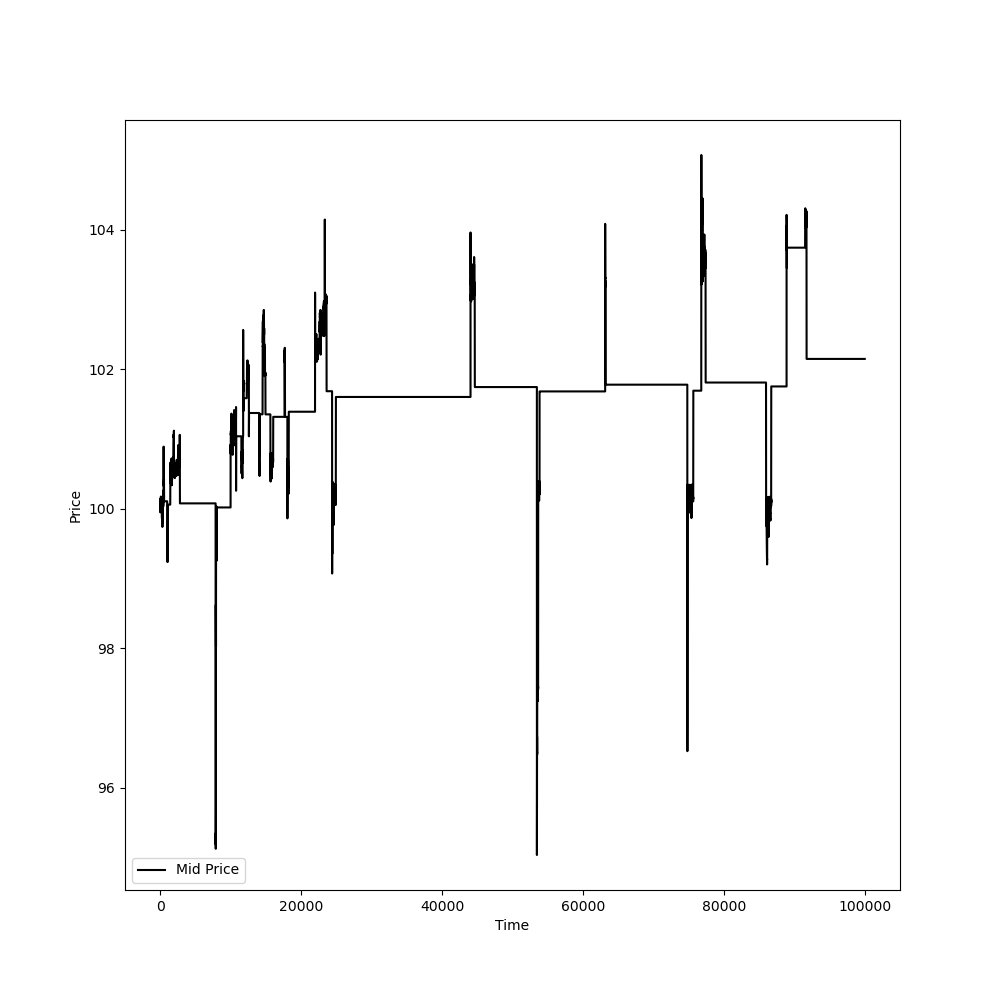
\includegraphics[width=7cm, height=7cm]{Dissertation/images/Mcg_final/full/mcg_10.png}
    \caption{20 of each agent}
    \label{fig:mcg_all_20}
  \end{subfigure}
  %
  \begin{subfigure}[b]{0.5\textwidth}
    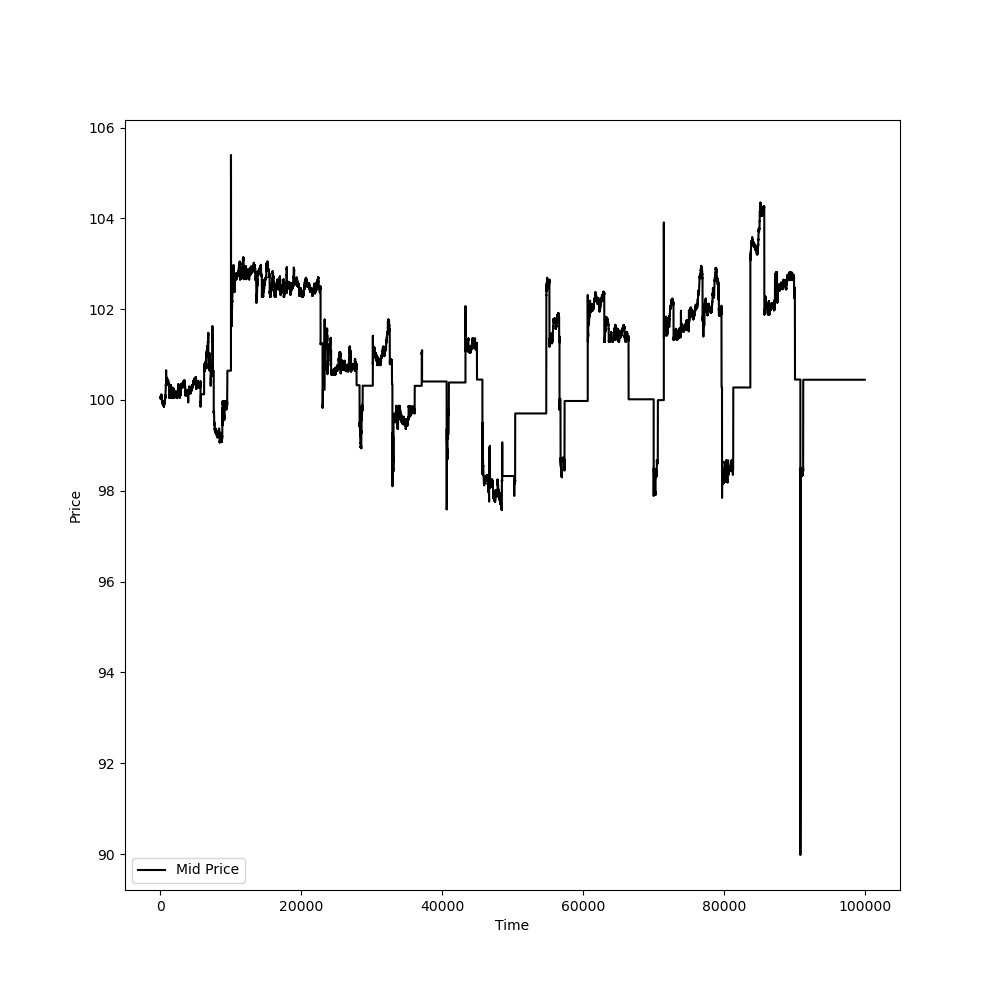
\includegraphics[width= 7cm, height= 7cm]{Dissertation/images/Mcg_final/full/mcg-20.png}
    \caption{40 of each agent}
    \label{fig:mcg_all_40}
  \end{subfigure}

  \begin{subfigure}[b]{0.5\textwidth}
    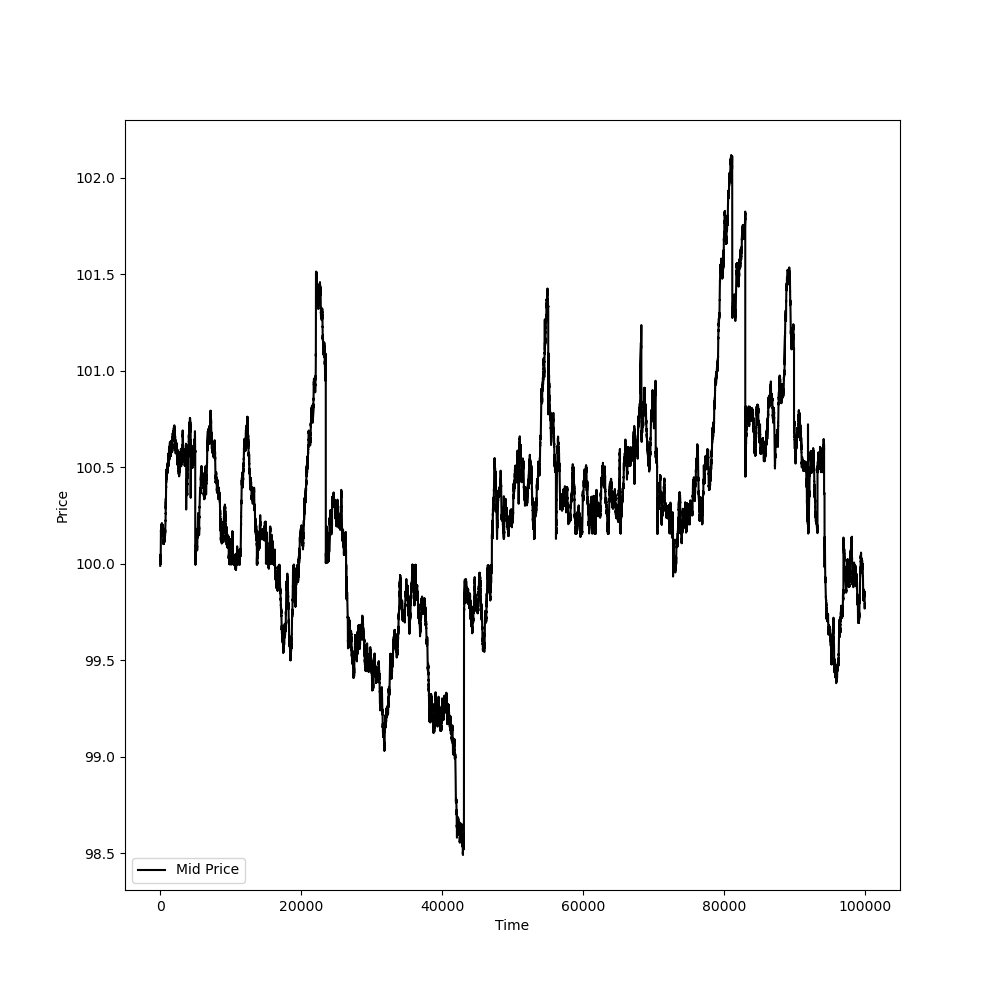
\includegraphics[width=7cm, height=7cm]{Dissertation/images/Mcg_final/full/mcg-30.png}   
    \caption{60 of each agent}
    \label{fig:mcg_all_60}
  \end{subfigure}
  %
  \begin{subfigure}[b]{0.5\textwidth}
    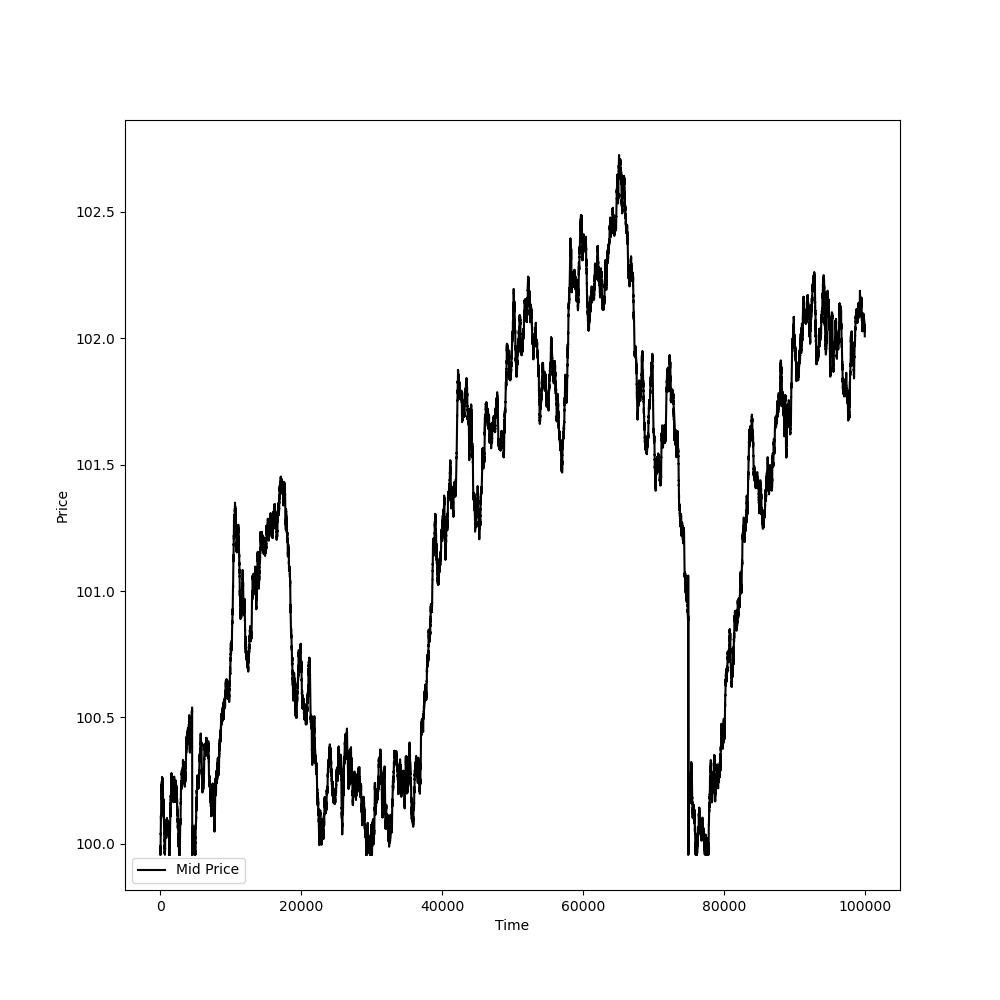
\includegraphics[width= 7cm, height= 7cm]{Dissertation/images/Mcg_final/full/mcg-40.png}
    \caption{80 of each agent}
    \label{fig:mcg_all_80}
  \end{subfigure}
\caption{Mid price Series of different number of agents in the market ran with 100,000 McG action-step} 
\end{figure}
\FloatBarrier

Similar to what we found with Oesch's market, In Figure \ref{fig:mcg_all_20} and Figure \ref{fig:mcg_all_40} when there are small number of agents in the market, we experience a market where there are unrealistic price patterns caused by the lack of Noise agents and unrealistic price spikes caused by Market maker and Liquidity consumer submitting large orders. On the other hand in Figure \ref{fig:mcg_all_80}, when there are a lot of agents in the market, the price will not cross the initial mid price and moves toward one direction over the whole experiment period with agents submitting at the best price moving it to one direction. 

\subsection{Noise agent and its crucial role in the simulated market}

Another interesting but not obvious result is that if there are no Noise agents in the market, the behaviour will not be as expected. Without the Noise agent, the mid-price of the whole market will be a flat line, regardless of the time-period of the experiment. This comes from a number of reasons: 

\begin{itemize}
  \item Mean Reversion trader will not submit an orders because there is no change in the value of the price, hence the standard deviation will be 0. This means that the price will already be at the moving average and will not trigger any conditions that the Mean reversion trader will submit an order.
  \item Momentum trader will also submit no orders because there is no change in price, hence no change in the momentum of the price. 
  \item This leads to the fact that only Liquidity consumer and Market maker that will submit orders. Liquidity consumer only submit market orders, hence no change in price will accord from its orders. Market maker only submits at best price, and since there are no other agents that will contribute to the change in price, there will be no deviation from the initial best price of the market. 
\end{itemize}

\section{Evaluation of Results}

\subsection{Oesch's configuration experiments}
In Chapter 5 we have successfully simulate a market in which the price pattern is in range of the original literature as well as a close mid-price return pattern. By doing this, we achieved part of our original goal which is implement the 3 out of 5 trading agents that Oesch's original paper claims to produce real market dynamics. In section 5.1.2 and 5.1.3, we also explored how the number of agents in the market and the price patterns in each market configuration. This gave us a better insight on the behaviour of Market makers and Liquidity consumer and how they react in different market conditions. In addition, in section 5.1.4 we also explored how the ratio of Noise agent in the market affects the price pattern and how it can create an unrealistic price pattern if there are less of them in the market. 

Overall, Chapter 5 provides us with a better insight on the three agents : Noise trader, Market maker and Liquidity consumer. However, there are areas that we would like to explore in the future. In Oesch's original conference paper, the literature took a deeper look into price impact on the market. This can be described as ``Market or price impact is the effect a trade has on the market price of a financial asset. An executed sell (buy) trade is usually associated with a fall (rise) in the market price." \cite{Oesch}. Oesch took a deeper look into how the ratio of these traders as well as how parameters of each agent affect the price impact function. Although this is a very interesting topic that we would like to explore, on top of return statistics analysis such as Kurtosis and volatility clustering which can be described as ``large changes in price tend to follow other large price changes" \cite{McGroarty}, it is beyond scope of this project due to time constraint. 

\subsection{McG configuration experiments}
In Chapter 6, we explored more deeply into the two frequency traders since we have established that the behaviour of the three traders can produce a similar price pattern compared with Oesch's original paper. In section 6.1.1, we explore how parameters should be adapt in order to properly implement the two frequency traders. In section 6.1.2, we explored the concept of price spikes from Johnson et al. \cite{Johnson} and McG\cite{McGroarty} where unfortunately, we were not able to mimic a price spike that is seen in the real market but did manage to reproduced the same behaviour between Mean Reversion trader and Momentum trader that causes the price spikes described in McG. 

In short, Chapter 6 provides us with a chance to explore the parameters and one of the unique feature of McG market that makes up a realistic market dynamics. In our perspective, we reached our goal for the project by implementing and adapt the McG agents so that they work with the BSE and was able to produce results that suggest the agents have similar behaviour to what is described in previous literature. This is consistent with our results in Chapter 3 and Chapter 4 where we tested the BSE integrity by comparing ZI-P, ZI-C and Sniper's behaviour with previous literature and Base Line results as well as the behaviour of individual agents to what is described in McG and Oesch. 

There are certainly interesting areas that could be improved and explored in detail in this project. The first is how close the final configuration is to McG. Because some parameters of McG were not given such as ratio of the agent and wealth calculation of the Momentum agent, it is possible that our implementation and McG's is different which outputs different values in the experiments. With more exploration, these parameters could certainly be improved with more experiments and exploration on the parameters effect on the market. In addition, although we were not able to mimic a full price-spike, the behaviour of Mean Reversion trader and Momentum trader is similar to what is described  in McG. With a deeper exploration into the parameters of the agent, a price spike can certainly be achieved. These are all areas that are beyond the scope due to the current time limit but are very interesting extensions for the current project. 

\chapter{Conclusion} 
\section{Project Summary}

This initial goal of the project is introduce realistic trading dynamics to the BSE. To a certain extent, the goal has been achieved since we have successfully shown a market similar to what is described in Oesch \cite{Oesch} and Minor Price Spikes which exhibits the behaviour of Mean reversion and Momentum traders. In addition, we have successfully implemented a new BSE which can handle more complex order types and shown the system integrity through the Base Line results of the three agents : ZI-P, ZI-C and Klapan's Sniper. In addition, we have shown that the behaviour of the five agent listed in McG (Market maker, Liquidity consumer, Mean reversion trader, Momentum trader and Noise trader) is implemented as to what is described by both McG and Oesch as well as adapting their parameters so that the behaviours are more suited for the current implementation of the BSE. 

\section{Challenges}
Two of the most important challenges of this project is the time constraint and hardware challenges. Because of COVID-19, we were only able run the experiments on a personal computer, which might not as be as powerful as the ones available at the university, limiting the experiment trials and total run-time of the McG. 

In addition, because many parameters of McG and Oesch was not given, this poses a huge challenge in the implementation stages of the trading agents and the market. The parameters of the agent, as shown in various sections of this paper, plays a huge role in determining the behaviour of an agent as well as the market as a whole. Many of the parameters of the agents and market, such as the number of agents and their ratio, has been chosen through trial and error as well as educated guess. Because all the agent behaviour have been shown to act as expected, it is a matter of how the market is setup and their parameters that determine the return statistics and how close it is to McG and Oesch's market. 

\section{Future work}
Apart of mimicking the markets shown in Oesch and McG there are also other areas which are interesting to explore. In the background chapter, we mentioned that the dominance of agents such as AA and ZI-P can certainly change with the market it is operating in. Because the markets in Oesch and McG has properties that real market has, by experimenting with AA and ZI-P in this market may give new insights on how the agents will react in the real market and how certain aspects of a real market dynamics may change the behaviour of the trading agents. 

In addition, it would also be interesting to do a more in-depth study of price spikes and what kind of scenarios would create these price spikes. As mentioned in the background, the research of this ultrafast extreme events are very relevant in this decade. This includes exploration on how each individual agents are contributing to the price spikes and how their parameters, as well as their ratios in the market, can further effect the occurrence of these events.  

\bibliographystyle{plain} % We choose the "plain" reference style
\bibliography{research} % Entries are in the "refs.bib" file

% \begin{appendices}
% \chapter{Individual Agents test results}
% Individual Agents test results 

% \end{appendices}

\end{document}
